% Puede generar borradores si omite la opción "final" de la clase.
% \documentclass{udpthesis}
\documentclass[final]{udpthesis}

% Establecemos el sistema para uso del español
% Babel ya esta cargado dentro de updthesis
\usepackage[T1]{fontenc}			%output
\usepackage[utf8]{inputenc}	%input
\usepackage{calc}
\usepackage{ifthen}
\usepackage{lmodern}
\usepackage{listings}
\usepackage{tikz}
\usetikzlibrary{shapes,arrows}
\usepackage{verbatim}
\usepackage{nomencl}
\usepackage{pgfplots} % fuer plots
\usepackage[external]{forest}
%jguzman
\usepackage{xspace} 




% Leyendas
\usepackage[font=footnotesize,labelfont=bf,labelsep=period]{caption}

% Agregue acá otros paquetes que le sean de utilidad
\usepackage{amsmath}	% Matemáticas\bigtriangleup
\usepackage{graphicx}	  % Gráficos
\usepackage[font=footnotesize,labelformat=simple]{subfig}
\usepackage[acronym]{glossaries}



\makeglossaries


\newglossaryentry{latex}
{
	name=latex,
	description={Is a mark up language specially suited for 
		scientific documents}
}

\newglossaryentry{maths}
{
	name=mathematics,
	description={Mathematics is what mathematicians do}
}

\newglossaryentry{formula}
{
	name=formula,
	description={A mathematical expression}
}

\newacronym{gcd}{GCD}{Greatest Common Divisor}
\newacronym{lcm}{LCM}{Least Common Multiple}




% Cambiamos el formato de las leyendas: finalizan en punto, y en negrita.
\captionsetup{labelsep=period,labelfont=bf}

% Habilitamos el uso de paréntesis al citar las figuras con subfiguras dentro, e.g., Fig. 1(a)
\renewcommand\thesubfigure{(\alph{subfigure})}
\renewcommand\thesubtable{(\alph{subtable})}
\newcommand{\subfigureautorefname}{\figureautorefname}


\lstset{
 % language=[LaTeX]TeX,
 breaklines=true,
 basicstyle=\tt\scriptsize,
 keywordstyle=\color{blue},
 identifierstyle=\color{black},
 commentstyle=\color{green!40!black},
 % frame 
 frame=tb,
 captionpos=t,
 xleftmargin=1em,
 numbersep=0.3em,
 % numbers=left,
 framexleftmargin=1.1em,
 framexrightmargin=0pt,
 % additional letters for accents in spanish
 literate=%
   {á}{{\'{a}}}1
   {é}{{\'{e}}}1
   {í}{{\'{i}}}1
   {ó}{{\'{o}}}1
   {ú}{{\'{u}}}1
   {ñ}{{\~{n}}}1
   {Ñ}{{\~{N}}}1
}


% Código
% Para generar código fuente usar listings.sty
%\usepackage{listings}
%\usepackage{tikz}
%\lstset{
%  language=[LaTeX]TeX,
%  breaklines=true,
%  basicstyle=\tt\scriptsize,
%  keywordstyle=\color{blue},
%  identifierstyle=\color{magenta},
%  commentstyle=\color{green!40!black},
%  % frame 
%  frame=tb,
%  captionpos=t,
%  xleftmargin=1em,
%  numbersep=0.3em,
%  numbers=left,
%  framexleftmargin=1.1em,
%  framexrightmargin=0pt,
%  % additional letters for accents in spanish
%  literate=%
%    {á}{{\'{a}}}1
%    {é}{{\'{e}}}1
%    {í}{{\'{i}}}1
%    {ó}{{\'{o}}}1
%    {ú}{{\'{u}}}1
%    {ñ}{{\~{n}}}1
%    {Ñ}{{\~{N}}}1
%}
%
%\renewcommand{\lstlistingname}{Código}% Listing -> Código
%\DeclareCaptionFormat{listing}{\rule{\dimexpr\linewidth\relax}{0.4pt}\par\vskip1pt#1#2#3}
%\captionsetup[lstlisting]{format=listing,singlelinecheck=false, margin=0pt,position=bottom}

% O para generar algoritmos en pseudocódigo usar algpseudocode.sty
\usepackage{algorithm}% http://ctan.org/pkg/algorithms
\usepackage{algpseudocode}

%\makeatletter
%\renewcommand{\ALG@name}{Algoritmo}% Algorithm -> Algoritmo
%\makeatother
%\captionsetup[algorithm]{font=footnotesize,labelsep=period}

\usepackage{cite}% Referencias (este paquete ordena y comprime las referencias)
\udptheme{EIT}

\newcommand{\uncm}{\vspace{1cm} }
\newcommand{\mediocm}{\vspace{0.5cm} }

%\newcommand{}{}
%\xspace This command decides whether to insert
% a space or not, usually this works well.


\newcommand{\www}		{\emph{www}\xspace}
\newcommand{\webs}		{\emph{webs}\xspace}
\newcommand{\web}		{\emph{web}\xspace}
\newcommand{\inet}		{\emph{Internet}\xspace}
\newcommand{\trie}		{\emph{trie}\xspace}
\newcommand{\online}	{\emph{online}\xspace}
\newcommand{\offline}	{\emph{offline}\xspace}
\newcommand{\cloudcomputing}{\emph{cloud computing}\xspace}

%  ~\ref{}
%  ~\cite{}



\newcommand{\webasccesslog}{\emph{webaccess log}\xspace}
\newcommand{\webasccess}{\emph{webaccess}\xspace}
\newcommand{\machinelearning}{\emph{Machine Learning}\xspace}
\newcommand{\hiddenmarkovmodels}{\emph{Hidden Markov Models}\xspace}
\newcommand{\losslessdatacompression}{\emph{Lossless Data Compression}\xspace}
\newcommand{\datacompression}{\emph{Data Compression}\xspace}
\newcommand{\lempelziv}{\emph{Lempel-Ziv}\xspace}

\newcommand{\menorEspacioItemize}{
	\setlength{\itemsep}{1pt}
	\setlength{\parskip}{0pt}
	\setlength{\parsep}{0pt}
	}




% SIGLAS todas con ttt
\newcommand{\LDC}{\texttt{LDC}\xspace}
\newcommand{\HMM}{\texttt{HMM}\xspace}
\newcommand{\VMM}{\texttt{VMM}\xspace}
\newcommand{\PPM}{\texttt{PPM}\xspace}
\newcommand{\DMC}{\texttt{DMC}\xspace}
\newcommand{\lzSieteOcho}{\texttt{LZ78}\xspace}
\newcommand{\lzSieteSiete}{\texttt{LZ77}\xspace}



% FOOTNOTES


\newcommand{\footnoteHuffman}{Los algoritmos de compresión aritméticos como el compresor de \emph{Huffman}, se basan en un modelo estadístico, es decir, un alfabeto y una cierta distribución de probabilidad de una fuente de datos. }
\newcommand{\footnoteGZIP}{gzip es un software libre GNU que reemplaza al programa \texttt{compress} de UNIX,~\url{http://www.gzip.org/}}


% REFERENCIAS
% a ideas / secciones / figuras


\newcommand{\refMLintro}{\ref{ch2:sec-machinelearning-seq-data}\xspace}
\newcommand{\refLDCmodelamiento}{\ref{sec-ldc-model-math}\xspace}





% citas
% prefijos
% LDC un papaer con relacion a compresion
% PDA un paper con relacion a predicion
% ML un paper con relacion a machine learming
\newcommand{\LDCMoghaddam}{\cite{Moghaddam2009}\xspace}
\newcommand{\MLPDASunila}{\cite{gollapudi2016practical}\xspace}
\newcommand{\MLGuller}{\cite{guller2015big}\xspace}
\newcommand{\MLkhanna}{\cite{khanna2015efficient}\xspace}
 %myHacks





\begin{document}




\frontmatter %% Inicio de la portada
%%%%%%%%%%%%%%%%%%%%%%%%%%%
\title{Modelo de Predicción Secuencial de Webaccess Log basado en el Algoritmo de Compresión LZ78 y Machine Learning}
%%%%%%%%%%%%%%%%%%%%%%%%%%%
% para precisar aún más su tema, use un subtítulo
%\subtitle{Subtítulo explicativo del tema}
\author{Jaime Guzmán} \email{mail@jguzman.cl} \date{2016}
%%%%%%%%%%%%%%%%%%%%%%%%%%%
%%%%%%%%%%%%%%%%%%%%%%%%%%%
% Profesor guía
\professor{Adín Ramirez}
% Comité
\committee{Francisco Claude}{Martin Gutierrez}
%%%%%%%%%%%%%%%%%%%%%%%%%%%
% Dedicatoria
\dedicatory{Dedicado a mi hijo, mis padres y las personas que no dejaron de apoyarme a pesar de las adversidades.}
%%%%%%%%%%%%%%%%%%%%%%%%%%%
% Agradecimientos
\acknowledgment{ % Nota redactada sobriamente en la cual se agradece a quienes han colaborado en la elaboración del trabajo. No puede exceder más de una página.

Mis primeras palabras de dedicatoria  y gratitud son para mi hijo Julian, mi hermano y mis padres, sin su apoyo incondicional en las buenas o malas decisiones que he tomado, siempre han estado para apoyarme, tal vez nunca hubiera podido terminar esto con el ritmo del trabajo y el estudio, pero ustedes siempre me motivaron, al igual que mi hermano.  Javier muchas gracias por ser mi más grande referencia en este mundo académico, espero presentar antes que termine su doctorado en Boston. También debo agradecer a mis trabajos que me han permitido financiar y lograr llegar hasta aquí, que ha costado mucho, muchas gracias  por ayudarme con el tiempo y facilidades para poder afrontar ciertos momentos en los que ha sido complicado continuar. Inmensamente agradecido a  Felipe Hermosilla y Jorge Cañon (Bice Vida - compañía de seguros), Max Díaz y Felipe Hrdina (RLGroup SPA - RatslabsIO\footnote{\url{http://www.ratslabs.io}}).

También agradezco a mis mentores y profesores guías: Adín Ramirez y Francisco Claude. Adín por darme la disciplina y enseñarme a escribir rigurosamente documentación de investigación y llevarme siempre más allá de lo que me he propuesto, como también ayudándome a abordar este tema con sus puntos de vistas y basto conocimiento, muchas gracias por su paciencia infinita para recibirme y llamarme la atención cuando desaparecía. También ha Francisco Claude por iniciarme en estos temas y motivarme, como también por un ser un gran referente en los temas de interés que abordado, probablemente sin sus consejos nunca habría intentado tomar un tema como éste, muchas gracias a ambos, ustedes me han inspirado enormemente. 

Finalmente debo agradecer a la Universidad Diego Portales, a sus administrativos y profesores que he ido conociendo en él camino, sin orden particular: Ximena Geoffroy, muchas gracias por su paciencia para escucharme y aconsejarme en todo momento, Loreto Montenegro, J. Frez, Sergio Mujica, Martin Gutierrez, Javier Pereira, Diego Dujovne, Jorge Elliot, todos han contribuido a que me guste más lo que estudié y trabajo día a día. También a mis amigos que hice durante la carrera y fuera de la universidad, por comprenderme y darme mucho ánimo para finalizar este trabajo y por último, muchas gracias María Paz haz sido fundamental en este proceso. }
% Abstract en inglés
\abstract{ Internet is growing every day and data volumes grow in the order of 
terabytes, for this reason it is of interest to use compression 
techniques for larger-scale processing of information with the fewest 
possible resources. Today there are various types of web: social networks, microbloging, web information, etc. The content provided to end 
users is not static and this allows them to create, contribute, and 
modify content, so Web Development Industry is constantly evolving to generate 
better solutions and friendly interaction with the users. 
Many of these new technologies have to deliver a better experience when browsing, the breakthrough has made it possible to create Web that are themselves intelligent and anticipating their behavior can go to, for example, decrease latency from a website and accessed or since navigate within a site with high concurrency; also from the point of view of the current web service patterns that are consumed immediately give a wide application area and provides a strategic aspect to the use of the information. While the growth of storage resources in the cloud is in full swing, networks don't grow at the same speed, which gives an area of interest to deepen.


So in this thesis we  propose the creation of a hybrid model between Machine Learning and Lossless Data Compression  for predict the next page that some user can access within a web; using training techniques and compression algorithms like well know \texttt{LZ78}, on a server Machine Learning. To this end we will work to create and study a predictive model that uses both areas and provide the results of the predictive model with integrated online component to any type of platform. }
% Resumen - Abstract en español
\resumen{ 	%El resumen no debe contener menos de 100 palabras ni mas de 300 palabras.

Internet crece exponencialmente  y los datos son generados en grandes volúmenes, en el orden de los \emph{Terabytes}. Hoy en día existen varios tipos de \emph{webs}: redes sociales, microbloging, \emph{web} informativas, etc. esto genera un interés en usar técnicas de compresión para realizar procesamiento a mayor escala de información con la menor cantidad de recursos posibles. El contenido proporcionado a los usuarios finales ya no es estático y esto permite que los mismos puedan  aportar, modificar ó eliminar contenido. Así  la industria del desarrollo web está en constante evolución para generar más variados recursos para ser usados. Muchas de estas nuevas tecnologías han permitido entregar mejor experiencia al momento de navegar en el lado del cliente, pero el gran avance realizado aún no permite crear \emph{web} que sean en sí inteligente por si misma y pueda ir anticipando la  navegación de un usuario o la recomendación de un contenido, tenemos los siguientes ejemplos; disminuir la latencia desde que se comienza a navegar una \emph{web} prediciendo los accesos futuros del usuario o aún mejor reconocer patrones discretos en la navegación de un usuario,  de un sitio concurrente; también desde el enfoque de los patrones de desarrollo \emph{web} actuales, los servicio  se consumen inmediatamente y dan una área de aplicación e integración extensa, aportando un aspecto estratégico al uso de la información con procesamiento inmediato. Si bien el crecimiento del almacenamiento de datos en la nube se encuentra en auge en la industria, las redes de telecomunicaciones  no crecen a la misma velocidad, lo cual genera un campo de interés para investigar. 

En este trabajo proponemos  la creación de un modelo híbrido entre \emph{Machine Learning} y Algoritmos de tipo \emph{Lossless Data Compression} para predecir la siguiente secuencias de acceso que usuario puede realizará dentro en una web; usando un modelo de navegación basado en un Algoritmo de Compresión como \texttt{LZ78}, sobre un servidor de Machine Learning. Con este propósito se trabajará para crear y estudiar un modelo predictivo que use ambas áreas y  ofrezca los resultados del modelo predictivo con una componente \emph{online} integrable a cualquier tipo de plataforma cliente. }
%%%%%%%%%%%%%%%%%%%%%%%%%%%
\makecover				 % Generamos la portada
\tableofcontents % tabla de contenido
\listoftables					% Indice de tablas
\listoffigures			 % Indice de figuras
\mainmatter	 			 % Inicio del contenido
% LA GRACI ES SER REPETITIVO SIN QUE SE NOTE.
%%%%%%%%%%%%%%%%%%%%%%%%%%%
% Capitulo I


\chapter[Introducción]{Introducción}\label{cap:ch1-intro}



%%%%%%%%%%
% Uno de los interes en poder crear un un aplicación de ambas areas es la convergenia de las areas en la cual un proceso de aprendizaje ó predicción secuencial se puede usar con ML y Compress data

% @TODO: SEGUIR TRABAJANDO EN ESTA BREVE INTRODUCCION
%En este tema convergen tres áreas, por un lado existe trabajo para crear estructuras eficientes para predicciones basadas en algoritmos de compresión, como es en el caso de~\cite{Claude2014}, y, por otro lado, el uso de algoritmos de aprendizaje para realizar clustering y predecir el comportamiento basado en el mismo contenido o en la distancia del contenido que visita el usuario actual al contenido clusterizado, como es el caso de ~\cite{Poornalatha2012}, inclusive se han utilizado modelos de Markov en ~\cite{Dongshan2002}  para poder modelar el comportamiento de la web.
%La tercera área son los Sistemas de Recomendación, la cual en este proyecto no se tocará pero si se mencionará el enfoque práctico que presenta área como un foco de múltiples implementaciones. 



\chapter[Introducción]{Introducción}
\label{ch:intro}

%chacharara
{

Los nuevos avances tecnológicos  y la inclusión de la ciencia de la computación en distintas campos han permitido hacer colecciones de datos muy grandes, las cuales se deben procesar, clasificar y analizar. Encontrar información útil dentro de estos grandes volúmenes de datos significa poder mejorar la decisiones a las que se pueden tomar dada a una base de conocimiento.

La minería de datos basado en web access se ha convertido en un área importante de investigación en los últimos años. Se puede utilizar para mejorar el rendimiento de la caché web, la detección de intereses de los usuarios y así recomendar páginas o bienes relacionados para los sitios web de comercio electrónico, mejorar los resultados de los motores de búsqueda  y por ejemplo personalizar el contenido de la web con las preferencias deseadas para el usuarios . En la predicción de navegación web logrando entender el patrón de navegación del usuario y luego la predicción de las páginas siguientes es el principal problema que buscamos solucionar. Con un sistema de predicción fiable podemos ver la siguiente acción de los usuarios de Internet y tomar acciones.

Normalmente se ocupa muchos algoritmos de Machine Learning para poder hacer predicciones en variadas áreas.  Hoy en día las aplicaciones en que los usuarios se enfrentan no pueden ser estáticas y sin tener un comportamiento que ayuden a predecir la forma en que actúan los usuarios. Esta área toma mucha relevancia al encontrarnos en una auge de la información generada por usuarios, redes sociales y variadas plataformas. Podemos mencionar que esta es una de las razones para poder requerir disponer de herramientas de análisis y predicción que nos permitan saber como se comporta usuarios sobre una web, conocer la frecuencia en que se accede a un recurso en Internet, etc.

El momento en que un usuario entre a un web se establece una conexión cliente-servidor. Una gran cantidad de servicios proporcionan datos de accesos de los usuarios que acceden, sobre estos mismos se puede realizar variadas investigaciones sobre como predecir cual es la siguiente página que podrá visitar.

%%%%%%Moghaddam_Kabir
Las predicciones en los registros de web access han atraído una atención significativa en los últimos años. Muchas técnicas de recuperación de datos  y algunos sistemas de personalización usan algoritmos de predicción. La mayoría de las aplicaciones actuales que predicen la siguiente página Web de un usuario tienen una componente en línea que hace la tarea de preparación de datos y una sección en línea que proporciona contenido personalizado a los usuarios en función de sus actividades de navegación actuales. En este trabajo se presenta un modelo de predicción en línea que se puede consumir como un servicio de API el cual da una integración ha variadas plataformas y sistemas que no tenga un componente en línea y con una buena precisión de la predicción. 
Nuestro algoritmo se basa en algoritmos LZ78 que están adaptados para modelar  y representar la navegación secuencia del usuario en una web. Nuestro modelo disminuye la complejidad computacional, que es un problema grave en el desarrollo de sistemas de predicción en línea. 


  }

%%%%%%Moghaddam_Kabir
%Web access prediction has attracted significant attention in recent years. Web prefetching and some personalization systems use prediction algorithms. Most current applications that predict the next user web page have an offline component that does the data preparation task and an online section that provides personalized content to the users based on their current navigational activities. In this paper we present an online prediction model that does not have an offline component and fit in the memory with good prediction accuracy. Our algorithm is based on LZ78 and LZW algorithms that are adapted for modeling the user navigation in web. Our model decreases computational complexities which is a serious problem in developing online prediction systems. A performance evaluation is presented using real web logs. This evaluation shows that our model needs much less memory than PPM family of algorithms with good prediction accuracy.

%Web mining has become an important research area in recent years. It can be used to improve the web cache performance[1, 2], Detecting the user interests and so recommending related pages or goods for e-commerce web sites [3], improving search engines results [4] , and personalizing the web content as the users like [5]. In web page prediction understanding the user navigation pattern and then predicting the next pages is the main problem. With a reliable prediction system we can see the next action of web users.






%When user requests inserted and deleted incrementally the online models are desirable. In this paper we present efficient techniques for modeling user navigation behavior. Our model is online so changes in user request patterns will update our prediction model incrementally.
%%%%%%%%%%%%%%%%

% 

% Nuestro intere es hacer que las rpecicciones sean modeladas por un compresaor de datos basado en Lempel ziv



%%%%%%%%%%
% Uno de los interes en poder crear un un aplicación de ambas areas es la convergenia de las areas en la cual un proceso de aprendizaje ó predicción secuencial se puede usar con ML y Compress data
% Cuando se hace el pio train se hace un entrenamiento de modelo lo que resulta ser es que genera el arbol que es un trie de LZ que será el predicto
% Una función de predición implementada con MLIB y PIO sería predict () en scala




%%%%%%% CONTEXTO PRELIMINAR 
\section{Contexto preliminar} 
\label{sec:preliminar}

% Idealmente aca explicar el problema

  La Web crece constantemente y por ende su infraestructura, también la información que podemos obtener de los  usuarios y  por consecuencia mayor concurrencia de los sistemas, la cual para los usuarios finales se traduce en un incremento de latencia y una mejor o peor experiencia de usuario. Paralelamente se suma un costo exponencial de recursos tanto en tecnologías de desarrollo como servicio que no son optimizados para poder dar una experiencia de usuario con calidad de servicio. Podemos reflexionar, entonces, que tener mayores recursos no mejorará el rendimiento, ni tampoco será lo óptimo para dar una calidad de servicio web ya que el ancho de banda de Internet no crecerá en la misma proporción.
   
  Adicionalmente, las tecnologías para la creación de web dinámicas y asíncronas han evolucionado a favor de traspasar la carga cliente.
  Hoy en día ya se poseen lenguajes y {framework} que disminuyen considerablemente la carga de un servidor, por lo cual, un buen servicio web es proveer una balanceada carga dentro del cliente y el servidor, pero cuando se poseen un gran volumen de datos es fundamental tomar decisiones que los recursos y lenguajes no cubren, es ahí el interés de dar inteligencia a servicios de la web.

  Interpretaremos que la manera en que un usuario navega es su comportamiento o patrón registrado en \emph{webacces log}, y que se pueden analizar, estudiar y modelar con algoritmos que tengan enfoques predictivos. 

  Sobre estos registros se pueden hacer representaciones eficientes como las realizadas por Claude \etal~\cite{Claude2014},  minería de datos para buscar \emph{Web Usage Mining} (WUM), el porque de hacer minería de datos radica en que cada día la web genera una innumerable cantidad de información, por lo cual usar algoritmos que se puedan opera de manera comprimida o con una representación lo más liviana posible es de interés ya que además de disminuir el espacio físico o recursos utilizados, se puede usar como un algoritmo de predicción y trabajar con una mayor cantidad de datos.
  
  Teniendo el conocimiento que los \emph{webaccess logs} se pueden estudiar de manera procesada o pre-procesada, ayudaría a ingenieros de desarrollo web y diseñadores de experiencia de usuarios, como también en general a mejorar la experiencia de usuario final, también disminuyendo por ejemplo la latencia en respuestas por parte de cada petición realizada, con técnicas de \emph{pre-fetching predictivo} en el lado del cliente.
  

  Actualmente, los sitios web han evolucionado de ser contenido estático a dinámico, también moderado por administradores a contenido orgánico creado por usuarios finales. Se debe poseer una adaptabilidad a la demanda o proveer información que permita adaptarse a los eventos, por lo tanto, hacer un estudio sobre esto y poder hacer integraciones en áreas como uso de algoritmos de compresión y \emph{Machine Learning} presenta un gran desafío. Independientemente del área, el problema común  se puede resolver pero se busca encontrar las fortalezas de cada área y usarlas en conjunto. 

  Durante este trabajo se usarán técnicas de compresión de datos, se utilizará una infraestructura y patrón de implementación para modelos de \emph{Machine Learning} como servicio. Adicionalmente toda la experimentación se llevará acabo ofreciendo los algoritmos y modelos como servicio basado en una Transferencia de Estado Representacional (\emph{REST}~\ref{concept-rest}), y así implementarlo en áreas productivas las cuales pueden presentar interés dando nuevos escenarios de estudio.


  La sesión de un usuario comienza cuando se conecta a un servicio web, éstas pueden ser páginas informativas, redes sociales, web dinámicas, contenido colaborativo, etc. Estableciendo dicha conexión a una página, se crea en ese momento una sesión de navegación automáticamente. Dado esto es posible almacenar datos muy relevantes los cuales son ''webaccess log'' ó registros de accesos web, durante el texto se mantendrán las referencias en inglés. Un ejemplo de \emph{webaccess log} es lo que se observa en la figura ~\ref{fig-ejemplo-webaccesslogbruto}:

\begin{figure}[tb]\label{fig-ejemplo-webaccesslogbruto} 
	\centering
	\begin{lstlisting}[frame=single,basicstyle=\ttfamily\tiny,]
	172.31.33.116 - - [26/Nov/2015:00:12:12 +0000] "HTTP/1.1" 200 1784 "http://localhost/home" 
	"Mozilla/5.0 (Linux; Android 5.1.1; SAMSUNG SM-G920I Build/LMY47X) 
	SamsungBrowser/3.2 Chrome/38.0.2125.102 Mobile Safari/537.36"
	172.31.33.116 - - [26/Nov/2015:00:12:12 +0000] "HTTP/1.1" 200 179333 "http://localhost/news" 
	"Mozilla/5.0 (Linux; Android 5.1.1; SAMSUNG SM-G920I Build/LMY47X) 
	SamsungBrowser/3.2 Chrome/38.0.2125.102 Mobile Safari/537.36"
	172.31.33.116 - - [26/Nov/2015:00:12:12 +0000] "HTTP/1.1" 200 24660 "http://localhost/health" 
	"Mozilla/5.0 (Linux; Android 5.1.1; SAMSUNG SM-G920I Build/LMY47X) 
	SamsungBrowser/3.2 Chrome/38.0.2125.102 Mobile Safari/537.36"
	172.31.33.116 - - [26/Nov/2015:00:15:12 +0000] "HTTP/1.1" 200 24604 "http://localhost/sports" 
	"Mozilla/5.0 (Linux; Android 5.1.1; SAMSUNG SM-G920I Build/LMY47X) 
	SamsungBrowser/3.2 Chrome/38.0.2125.102 Mobile Safari/537.36"
	172.31.33.116 - - [26/Nov/2015:00:20:12 +0000] "HTTP/1.1" 200 4860 "http://localhost/home" 
	"Mozilla/5.0 (Linux; Android 5.1.1; SAMSUNG SM-G920I Build/LMY47X) 
	SamsungBrowser/3.2 Chrome/38.0.2125.102 Mobile Safari/537.36"
	172.31.33.116 - - [26/Nov/2015:00:22:19 +0000] "HTTP/1.1" 200 4841 "http://localhost/finances" 
	\end{lstlisting}
	
	
	
	\caption{Ejemplo de un \emph{webaccess Log} de un servidor Apache.}
	\label{fig:accesslog-apache-teleton}
\end{figure}


  En la Figura \ref{fig-ejemplo-webaccesslogbruto} nos entrega mucha información interesante como la \texttt{IP} desde donde se conecta, el tipo de navegador, el dispositivo si es un teléfono inteligente o un navegador de escritorio, la fecha en que se realizó el acceso y también lo más relevante el destino del usuario.
  
  
  
  




\section{Definición del Problema}


El problema de la Predicción, ha surgido hace años y diversos investigadores han trabajado con distintos enfoques. Rissman y Langdom en los laboratorios Bell al realizar pruebas con un robot y hacer un experimento con un robot que tiraba una moneda compitiendo con humano, realizaba todos los calculos markovianos y calculos de las probabilidades condicionales para que cierto evento ocurra, a diferencia del sujeto que solo estaba esperando un resultado.

Predecir no es trivial, pero si podemos llegar a cercanos y minimizar el error de equivocarnos. Sin embargo, dos áreas han tratado de resolver el problema, LDC y Machine Learning de manera separada. Por parte de LDC los mayores problemas son que los predictores funcionan totalmente desconectados y no dan una de disponibilidad inmediata de los resultados, en cambios en el área de Machine Learning debemos crear un modelo para entrenar y luego poder generar una función predictiva.

Planteamos el problema de poder resolver tener un modelos híbrido juntando los patrones de cada área y disponerlo como un servicio inmediato dando una predictibilidad inmediata que hoy en la industria es necesaria para poder hacer útiles estos algoritmo y dar un valor a los avances.

 




% @TODO: SEGUIR TRABAJANDO EN ESTA BREVE INTRODUCCION
%En este tema convergen tres áreas, por un lado existe trabajo para crear estructuras eficientes para predicciones basadas en algoritmos de compresión, como es en el caso de~\cite{Claude2014}, y, por otro lado, el uso de algoritmos de aprendizaje para realizar clustering y predecir el comportamiento basado en el mismo contenido o en la distancia del contenido que visita el usuario actual al contenido clusterizado, como es el caso de ~\cite{Poornalatha2012}, inclusive se han utilizado modelos de Markov en ~\cite{Dongshan2002}  para poder modelar el comportamiento de la web.
%La tercera área son los Sistemas de Recomendación, la cual en este proyecto no se tocará pero si se mencionará el enfoque práctico que presenta área como un foco de múltiples implementaciones. 







%Algoritmos como serivcio
\section{Algoritmos como servicio web }

	Los avances en el desarrollo de nuevas tecnologías que brinden mejores experiencias en su uso día a día, deriva en cómo podamos llevar varios escenarios idealizados a implementaciones empresariales reales. Es bastante común encontrar librerías que son bastante útiles para hacer Minería de Datos, agrupación y muchas operaciones que pueden recurrir en cálculos muy complejos, pero no se pueden ofrecer como servicio. Ya en pleno auge de las infraestructuras en la nube, la capacidad de cómputo que se puede alcanzar no es un problema como antes lo era para un Científico de Datos.


	Una \emph{API} es un interfaz de programación de Aplicaciones que nos permiten intermediar el \emph{Servicio $A$} con el \emph{Servicio $B$}. Respectivamente $A$ puede ser el proveedor y $B$ el demandante del servicio. Si quisiéramos analizar datos que se encuentran dentro de un servidor específico, estos se podrían consumir por esta interfaz. Existen variados clientes que nos permiten ayudar en esta comunicación, incluso se pueden utilizar por una terminal de {Unix} que es posible dialogar mediante el programa \emph{curl}.
	
	Ya se dispone de infraestructura como servicio (\emph{IaaS}) , software como servicio (\emph{SaaS}), plataformas como servicios (\emph{PaaS}). Dado lo anterior ofrecer estos algoritmos para hacer que las soluciones de desarrollo den valor agregado a la experiencia requerida por el usuario final. Por esto hemos decidido utilizar una librería y {framework} que nos de esta posibilidad. Ofrecer algoritmos a la industria como un servicio que ayuda de manera eficiente e Inteligente desarrollado como una API REST, que permitirá una fácil integración. 
	
	Todas las ventajas de este patrón son heredados de las características que ofrece una API, interoperabilidad, evitar problemas de Infraestructura, Resiliencia de Datos, Persistencia de Datos, Análisis y Procesamiento sin afectar un curso operacional de una aplicación. Un ejemplo claro de esto es el análisis de datos en sistemas legados los cuales en plan de mejoras, no poseen la compatibilidad para poder realizarlo. Por otro lado, los algoritmos de compresión o algoritmos de \emph{Machine Learning} tienden a ser muy complejos de implementar o ocupan muchso recursos y este hecho pueden ser la razón para no implementarlos. 
	
	
	
	




%introducción a las Prediccion


\section{Predecir con \emph{PredictionIO}}

  	
En esta sección se presenta formalmente el ambiente de desarrollo que se utilizará durante este trabajo. \emph{PredictionIO} es un servidor de \emph{Machine Learning} de código abierto para Científico de Datos y Desarrolladores que permite crear motores de predicción para aplicaciones en producción, con un bajo tiempo de entrenamiento y despliegue. Principalmente está construido en \emph{Apache Spark, HBase} y \emph{Spray}. 

Este ambiente de trabajo se encuentra en un maduración estable y constante que permite tanto disponer servidores con motores predictivos, como también toda una infraestructura distribuida para hacer que complejos algoritmos que sean utilizados para solucionar problemas reales de mayor escala.



% PIO, tiene practicamente todo armadao, ello no hicieron nada nuevo ... solo juntaron  todo...



% He estado investigando y revisando documentación, Yelp, Skype, Hubot de github y otras implementaciones tienen usando prediction.io




% La otra opción es meterle a este "DASE" un algoritmo  que mezcle una representación de cadenas de markov mezclado con LZ78. no se en que punto mezclarlo en el diccionario, o la verdad es como hacer el compresor sea "mas inteligente", encontré un papaer que te adjunto en el cual usan lz78 y lzw, esta interesante ya que le hacen un acercamiento mas al tema de de ser un predictor online.


% Ahora entiendo que la cadenas de markov son y se han ocupado para las predicciones, pero no veo la necesidad de ocuparlas mayormente. Adin me inisiste en que le de una vuelta.... pero mi sensación  es que tengo separada las ideas en dos extremos. 

% Ya revise Suffix Tree para predicciones LZ77 y LZW, también PPM y HMM.

 
 



\subsection{Arquitectura DASE}


Un motor de predicción es un tipo de proceso en \emph{Machine Learning}. Siguiendo una arquitectura de tipo \emph{DASE}, contendríamos los siguientes componentes.



\begin{itemize}

  \item\label{dase-datasource} \textbf{ $[D]$ Data Source y Data Preparator}. Los Data Source leen la data desde la entrada original y la transforman en un formato deseado para hacer análisis de estos. En cambio \emph{Data Preparator} pre-procesa la información y la reenvía a los algoritmos para   hacer el modelo de entrenamiento.


  \item\label{dase-algoritmo} \textbf{ $[A]$ Algoritmo}. Los componentes de \emph{PredictionIO}, dada sus librerías incluyen algoritmos de \emph{Machine Learning}, estos, pueden ser provistos por \emph{Apache Spark} o se pueden incluir algoritmos propios como también de terceros.
    Adicionalmente a los algoritmos podemos asignarle parámetros, para determinar como debiese ser construido el motor ó si es requerido para un cierto algoritmo.



  \item\label{dase-servicio} \textbf{ $[S]$ Servicio}. El componente servicio toma las consultas ó \emph{queries} de predicción y retorna los resultados, en nuestro modelo propuesto en la etapa experimental veremos el siguiente símbolo de una secuencia. 
  Si el motor de predicción tiene múltiples algoritmos, combinará los resultados en uno. Adicionalmente, la lógica específica de negocios puede ser añadida para especificar aún más el resultado final. 
 
  \item\label{dase-eval} \textbf{ $[E]$ Evaluación de Métricas}.
Las métricas de evaluación cuantifican la precisión de la predicción con una puntuación numérica. Puede ser utilizado para la comparación de algoritmos o ajustes de los parámetros del algoritmo.
\end{itemize}




  \tikzstyle{decision} = [diamond, draw,text width=4.5em, text badly centered, node distance=2.5cm, inner sep=0pt]
  \tikzstyle{block} = [rectangle, draw,text width=5em, text centered, rounded corners, minimum height=4em]
  \tikzstyle{line} = [draw, very thick, color=black!50, -latex']
  \tikzstyle{cloud} = [draw, ellipse, node distance=2.5cm,
  minimum height=2em]


\begin{figure}[t]
	\centering	
	\resizebox{0.8\textwidth}{!}{% <------ Don't forget this %
	
		\begin{tikzpicture}[scale=1, node distance = 2.5cm, auto]
		% Place nodes
		
		\node [block] (init) {Data de la Aplicación};
		\draw [color=gray,thick](1.3,1) rectangle (11.2,-3.5);    
		
		\node [block,right of=init] 		  (datasource) {Data Source};
		\node [block,right of=datasource]     (datapreparator) {Data Preparator};
		\node [block,right of=datapreparator] (alg1) {Algoritmo };
		\node [block,right of=alg1] 		  (serving) {Servicio};
		\node [block,below of=serving] 		  (evalmetric) {Evaluación Métrica};
		\node [block,right of=serving] 		  (resultpredict) {Resultado Predicción};
		\node [block,below of=resultpredict]  (resulteval) {Resultado Evaluación};
		
		\path [line] (init) -- (datasource);
		\path [line] (datasource) -- (datapreparator);
		\path [line] (datapreparator) -- (alg1);
		\path [line] (alg1) -- (serving);
		\path [line] (serving) -- (evalmetric);
		\path [line] (serving) -- (resultpredict);
		\path [line] (evalmetric) -- (resulteval);    
		
		\end{tikzpicture}
	}
	\caption{Diagrama de componentes Arquitectura DASE.}
	\label{fig:arquitectura-dase}
\end{figure}



\vspace{1cm}

\emph{PredictionIO} ayuda a tener componentes muy modulares, las que ya hemos descrito como  arquitectura \emph{DASE} (\ref{fig:arquitectura-dase})  que puede construir modelos de predicción de manera sencilla y ya contando con toda la arquitectura y algoritmos de \emph{MLIB}\footnote{Machine Learning Library Apache Spark, \url{http://spark.apache.org/mllib/}} de \emph{Apache Spark}. También poder integrarlos con gran facilidad a cualquier sistema o plataforma, por ejemplo, es posible elegir cual de todos los componentes se podrá desplegar al momento de crear un \emph{Engine} (Motor de Predicción.)



\vspace{0.5cm}
\subsection{Despliegue de motor de predicción}

  Un \emph{Motor de predicción} pone todos los componentes del diseño de arquitectura \emph{DASE} en un estado especifico de despliegue 
  \begin{enumerate}
  		\setlength{\itemsep}{1pt}
  		\setlength{\parskip}{0pt}
  		\setlength{\parsep}{0pt}
    \item Data Source
    \item Data Preparator
    \item Uno o más Algoritmos generadores de Modelos
    \item Un Servicio 
  \end{enumerate}

  Si se especifica más de un algoritmo, cada uno de los resultados de los modelos de predicción se entregará para ser consumido por cualquier cliente.
  Cada \emph{motor de predicción} procesa los datos y construye un modelos de forma independiente. Por lo tanto, todos los motores de predicción que usaremos sirven a su propio conjunto de resultados. Por ejemplo, se puede desplegar dos \emph{motores predictivos} para una aplicación móvil: uno para recomendar noticias a los usuarios y otro para sugerir nuevos amigos a los usuarios.


\vspace{1cm}
\subsection{Evaluación del motor de predicción }

  Para evaluar el \emph{Accuracy} de un motor de predicción, se debe especificar la métrica seleccionad cuando se corre el motor de evaluación, en los capítulos experimentales se verá como se generan métricas y como se desempeña esta métrica para ser evaluada.











\subsection{Modelamiento de eventos}

%https://docs.prediction.io/datacollection/eventmodel/




  El modelamiento de eventos es fundamental para un predictor \emph{online}, el hecho de poder llevar un vector con ciertas propiedades característica\footnote{Característica de un cierto dataset para entrenar.} de una representación vectorial del mundo del \emph{Machine Learning} a un modelamiento secuencial, es en realidad el modelamiento que se debe realizar de como  tener las muestras de datos para generar \emph{Resilient Distributed Dataset} (\texttt{RDD}) que son un parte principal de nuestro ambiente de trabajo con \emph{PredictionIO} para poder acceder posterior o inmediatamente. 

  Un evento lo definiremos como entidad que nos permite dar una representación temporalizada de información que será procesada por un motor de predicción. Analizaremos los eventos que un usuarios realiza para poder acceder a una web. Adicionalmente cuando cada usuario ingresa a una web automáticamente este genera una sesión, desde que que llega hasta que abandona la web.

  Usaremos un \emph{dataset} con información que esta totalmente depurada y recuperada de los \emph{access log} (provista por Claude \etal~\cite{Claude2014}), los cuales a efectos de temporalidad solo nos interesa conocer la secuencialidad de estos accesos.
  


%Poner algo mas matematico.
% EVENT API 
% https://docs.prediction.io/datacollection/eventapi/

  El modelamiento que realizaremos contempla los siguientes campos :

    \begin{itemize}
    		\setlength{\itemsep}{1pt}
    		\setlength{\parskip}{0pt}
    		\setlength{\parsep}{0pt}
      \item Tipo de Evento: Visitar
      \item Entidad que ejecuta el evento: Usuario
      \item Propiedades:
          \begin{enumerate}
          		\setlength{\itemsep}{1pt}
          		\setlength{\parskip}{0pt}
          		\setlength{\parsep}{0pt}
            \item Página actual
            \item Página siguiente
            \item Cierre de Sesión
          \end{enumerate}
    \end{itemize}



    El interés de tener un modelo totalmente atómico es poder contemplar la información que nos entrega, destacando sus variables y propiedades como restricciones.



\subsection{Ventajas de PredictionIO }


  Es posible mezclar y aplicar distintas característica, si el modelo no puede ser persistido por \emph{PredictionIO} automáticamente. Se requiere un objeto  heredado de una clase que permita lograr la persistencia en memoria, esto permite cargar el modelo persistentemente e instanciar automáticamente durante la ejecución del motor de predicciones.

  % Tenga en cuenta que los modelos generados por PAlgorithm no pueden ser persistieron automáticamente por naturaleza y deben implementar estas características, si se desea modelo de persistencia.


  Comprendiendo el concepto de \emph{Resilient Distributed Dataset} (\texttt{RDD} \ref{concept-RDD}), ésta es la abstracción básica de \emph{Apache Spark}, aún más, esto es una de las grandes cualidades de PredictionIO, ya que no solamente podemos disponer de una máquina para hacer estudios o implementar algoritmos, este servidor de \emph{Machine Learning} permite, gracias a sus componentes poder hacer un cluster para entregar mayor eficiencia acorde a los datos o algoritmo a implementar.

  Ya hemos mencionado que los \texttt{RDD} son una representación inmutable, una colección divida de elementos que pueden ser operadas en paralelo. Internamente cada \texttt{RDD} tiene cinco principales propiedades:


  \begin{enumerate}
    \item Una lista de particiones.
    \item Una función para procesar cada porción de datos.
    \item Una lista de dependencias en otros \texttt{RDD}. 
    \item Opcionalmente una partición de un \texttt{RDD} puede ser representada como una combinación de llave y valor. 
    \item Una lista optativa de los lugares preferidos para calcular cada una dividida en (por ejemplo, lugares de bloque para un archivo \emph{HDFS}); para procesamiento en \emph{Clustering}.

  \end{enumerate}
  




% https://docs.prediction.io/templates/recommendation/customize-serving/


















%Se consideran y ex- plican detalladamen- te todos los concep- tos, teor ́ıas, y aspec- tos pertinentes al te- ma tratado.
%El marco teo ́rico con- cuerda con los ob jeti- vos y el tipo de traba- jo.











\section{Descripción del Contenido}

%Ejemplo :

%This paper is organized as follows. We begin in Section 2 with some preliminary defi- nitions. In Section 3, we present six VMM prediction algorithms. In Section 4, we present the experimental setup. In Sections 5-6, we discuss the experimental results. Part of the experimental related details are discussed in Appendices A-C. In Section 7, we discuss the related work. In Section 8, we conclude by introducing a number of open problems raised by this research. Note that the source code of all the algorithms we consider is available at http://www.cs.technion.ac.il/~ronbeg/vmm.




\section{Contexto preliminar} 
\label{sec:preliminar}

% Idealmente aca explicar el problema

  La Web crece constantemente y por ende su infraestructura, también la información que podemos obtener de los  usuarios y  por consecuencia mayor concurrencia de los sistemas, la cual para los usuarios finales se traduce en un incremento de latencia y una mejor o peor experiencia de usuario. Paralelamente se suma un costo exponencial de recursos tanto en tecnologías de desarrollo como servicio que no son optimizados para poder dar una experiencia de usuario con calidad de servicio. Podemos reflexionar, entonces, que tener mayores recursos no mejorará el rendimiento, ni tampoco será lo óptimo para dar una calidad de servicio web ya que el ancho de banda de Internet no crecerá en la misma proporción.
   
  Adicionalmente, las tecnologías para la creación de web dinámicas y asíncronas han evolucionado a favor de traspasar la carga cliente.
  Hoy en día ya se poseen lenguajes y {framework} que disminuyen considerablemente la carga de un servidor, por lo cual, un buen servicio web es proveer una balanceada carga dentro del cliente y el servidor, pero cuando se poseen un gran volumen de datos es fundamental tomar decisiones que los recursos y lenguajes no cubren, es ahí el interés de dar inteligencia a servicios de la web.

  Interpretaremos que la manera en que un usuario navega es su comportamiento o patrón registrado en \emph{webacces log}, y que se pueden analizar, estudiar y modelar con algoritmos que tengan enfoques predictivos. 

  Sobre estos registros se pueden hacer representaciones eficientes como las realizadas por Claude \etal~\cite{Claude2014},  minería de datos para buscar \emph{Web Usage Mining} (WUM), el porque de hacer minería de datos radica en que cada día la web genera una innumerable cantidad de información, por lo cual usar algoritmos que se puedan opera de manera comprimida o con una representación lo más liviana posible es de interés ya que además de disminuir el espacio físico o recursos utilizados, se puede usar como un algoritmo de predicción y trabajar con una mayor cantidad de datos.
  
  Teniendo el conocimiento que los \emph{webaccess logs} se pueden estudiar de manera procesada o pre-procesada, ayudaría a ingenieros de desarrollo web y diseñadores de experiencia de usuarios, como también en general a mejorar la experiencia de usuario final, también disminuyendo por ejemplo la latencia en respuestas por parte de cada petición realizada, con técnicas de \emph{pre-fetching predictivo} en el lado del cliente.
  

  Actualmente, los sitios web han evolucionado de ser contenido estático a dinámico, también moderado por administradores a contenido orgánico creado por usuarios finales. Se debe poseer una adaptabilidad a la demanda o proveer información que permita adaptarse a los eventos, por lo tanto, hacer un estudio sobre esto y poder hacer integraciones en áreas como uso de algoritmos de compresión y \emph{Machine Learning} presenta un gran desafío. Independientemente del área, el problema común  se puede resolver pero se busca encontrar las fortalezas de cada área y usarlas en conjunto. 

  Durante este trabajo se usarán técnicas de compresión de datos, se utilizará una infraestructura y patrón de implementación para modelos de \emph{Machine Learning} como servicio. Adicionalmente toda la experimentación se llevará acabo ofreciendo los algoritmos y modelos como servicio basado en una Transferencia de Estado Representacional (\emph{REST}~\ref{concept-rest}), y así implementarlo en áreas productivas las cuales pueden presentar interés dando nuevos escenarios de estudio.


  La sesión de un usuario comienza cuando se conecta a un servicio web, éstas pueden ser páginas informativas, redes sociales, web dinámicas, contenido colaborativo, etc. Estableciendo dicha conexión a una página, se crea en ese momento una sesión de navegación automáticamente. Dado esto es posible almacenar datos muy relevantes los cuales son ''webaccess log'' ó registros de accesos web, durante el texto se mantendrán las referencias en inglés. Un ejemplo de \emph{webaccess log} es lo que se observa en la figura ~\ref{fig-ejemplo-webaccesslogbruto}:

\begin{figure}[tb]\label{fig-ejemplo-webaccesslogbruto} 
	\centering
	\begin{lstlisting}[frame=single,basicstyle=\ttfamily\tiny,]
	172.31.33.116 - - [26/Nov/2015:00:12:12 +0000] "HTTP/1.1" 200 1784 "http://localhost/home" 
	"Mozilla/5.0 (Linux; Android 5.1.1; SAMSUNG SM-G920I Build/LMY47X) 
	SamsungBrowser/3.2 Chrome/38.0.2125.102 Mobile Safari/537.36"
	172.31.33.116 - - [26/Nov/2015:00:12:12 +0000] "HTTP/1.1" 200 179333 "http://localhost/news" 
	"Mozilla/5.0 (Linux; Android 5.1.1; SAMSUNG SM-G920I Build/LMY47X) 
	SamsungBrowser/3.2 Chrome/38.0.2125.102 Mobile Safari/537.36"
	172.31.33.116 - - [26/Nov/2015:00:12:12 +0000] "HTTP/1.1" 200 24660 "http://localhost/health" 
	"Mozilla/5.0 (Linux; Android 5.1.1; SAMSUNG SM-G920I Build/LMY47X) 
	SamsungBrowser/3.2 Chrome/38.0.2125.102 Mobile Safari/537.36"
	172.31.33.116 - - [26/Nov/2015:00:15:12 +0000] "HTTP/1.1" 200 24604 "http://localhost/sports" 
	"Mozilla/5.0 (Linux; Android 5.1.1; SAMSUNG SM-G920I Build/LMY47X) 
	SamsungBrowser/3.2 Chrome/38.0.2125.102 Mobile Safari/537.36"
	172.31.33.116 - - [26/Nov/2015:00:20:12 +0000] "HTTP/1.1" 200 4860 "http://localhost/home" 
	"Mozilla/5.0 (Linux; Android 5.1.1; SAMSUNG SM-G920I Build/LMY47X) 
	SamsungBrowser/3.2 Chrome/38.0.2125.102 Mobile Safari/537.36"
	172.31.33.116 - - [26/Nov/2015:00:22:19 +0000] "HTTP/1.1" 200 4841 "http://localhost/finances" 
	\end{lstlisting}
	
	
	
	\caption{Ejemplo de un \emph{webaccess Log} de un servidor Apache.}
	\label{fig:accesslog-apache-teleton}
\end{figure}


  En la Figura \ref{fig-ejemplo-webaccesslogbruto} nos entrega mucha información interesante como la \texttt{IP} desde donde se conecta, el tipo de navegador, el dispositivo si es un teléfono inteligente o un navegador de escritorio, la fecha en que se realizó el acceso y también lo más relevante el destino del usuario.
  
  
  
  




\section{Definición del Problema}


El problema de la Predicción, ha surgido hace años y diversos investigadores han trabajado con distintos enfoques. Rissman y Langdom en los laboratorios Bell al realizar pruebas con un robot y hacer un experimento con un robot que tiraba una moneda compitiendo con humano, realizaba todos los calculos markovianos y calculos de las probabilidades condicionales para que cierto evento ocurra, a diferencia del sujeto que solo estaba esperando un resultado.

Predecir no es trivial, pero si podemos llegar a cercanos y minimizar el error de equivocarnos. Sin embargo, dos áreas han tratado de resolver el problema, LDC y Machine Learning de manera separada. Por parte de LDC los mayores problemas son que los predictores funcionan totalmente desconectados y no dan una de disponibilidad inmediata de los resultados, en cambios en el área de Machine Learning debemos crear un modelo para entrenar y luego poder generar una función predictiva.

Planteamos el problema de poder resolver tener un modelos híbrido juntando los patrones de cada área y disponerlo como un servicio inmediato dando una predictibilidad inmediata que hoy en la industria es necesaria para poder hacer útiles estos algoritmo y dar un valor a los avances.

 



\chapter[Conceptos Básicos]{Conceptos básicos y trabajos relacionados} \label{ch:Conceptos-Basicos}





En este capítulo se explicarán brevemente los conceptos principales que se usarán en los siguientes capítulos:


\section{Conceptos}

\subsection{Access Log}\label{concept-accesslog}

Los \emph{Access Log} son registros que se almacenan en un servidor, los cuales dependiendo del servidor, sistema operativo y las configuraciones del ambiente pueden tener mayor o menor información. Cuando los usuarios acceden a diversos sitios web, estos registros dejan una gran cantidad de información, un ejemplo se puede ver en la Figura~\ref{fig:accesslog-apache-teleton}. Si se extraen de forma correcta se puede obtener patrones de navegación de usuarios. 


\subsection{Árboles Trie} \label{concept-trie}

Los \emph{trie} son un tipo de árbol de prefijos, estructuras de datos en forma de árbol que almacenan datos en sus nodos y es muy fácil la recuperación de información de estos. Se caracterizan por ser un conjunto de llaves que se representan en el árbol y sus nodos internos representan la información, en nuestro caso una secuencia de acceso o un símbolo (secuencia de largo 1). 

Un árbol es una estructura general de nodos recursivos. Hay muchos tipos de árboles. Los populares son árbol binario y el árbol balanceado. Un \emph{trie} es conocido por muchos nombres incluyendo árbol prefijo, árbol de búsqueda digital, árbol de la recuperación (de ahí el nombre de \textquotedbl \emph{trie}\textquotedbl, por la palabra del inglés recuperación, \emph{retrieval}).

Cada tipo de árbol tiene distinta finalidad, estructura y comportamiento. Por ejemplo, un árbol binario almacena una colección de elementos comparables (por ejemplo, números). Por lo tanto, se puede utilizar para almacenar un conjunto de números, o al índice de otros datos que pueden ser representados por los números (por ejemplo, objetos que pueden ser \emph{hash}). Su estructura está ordenada por lo que se puede buscar rápidamente para encontrar nodo. Otras estructuras de árbol, como un árbol balanceado son similares en principio al \emph{trie} que se implementará en la etapa experimental.

Un \emph{trie} representa una forma  estructurada de nodos, la cual puede almacenar secuencias. % (ver el artículo de wiki). 
Es muy diferente cuando almacena secuencias de valores en lugar de valores individuales. Cada nivel representa un incremento en la altura del árbol.
%'¿cuál es el valor del punto I de la lista de entrada'. Esto es diferente a un árbol binario que compara el valor buscado único a cada nodo.


Durante este trabajo mostraremos que nuestro modelo de predicción usa un \emph{trie}, para representar un diccionario, en los cuales podemos señalar las siguientes operaciones disponibles:

	\begin{itemize}	
		\item \textbf{findByPrefix(x):}  Retornar una una lista de todos los nodos hasta llegar a un nodo que posea un \emph{String} de parámetro equivalente a $x$.
		
		\item \textbf{contains(x):} Retornar una lista de nodos intermedios hasta que el contenido del nodo final sea hoja o el intermedio corresponda a valor de la secuencia \emph{String} $x$.
		
		\item \textbf{remove(x):} Retorna \emph{true} o \emph{false} cuando es posible remover el nodo con el contenido equivalente a $x$.
		
		\item \textbf{pathTo(x):} Retorna una lista de nodos hasta llegar a un nodo que posea el contenido equivalente del valor $x$.
	\end{itemize}







\subsection{Alfabeto} \label{concept-alphabet}

Un alfabeto es un conjunto ordenado de elementos. Una de sus características es que la cantidad de elementos puede ser de valores finitos y discreto lo representaremos por $\Sigma$ y una de las características básica de este alfabeto es consiste en símbolos $\sigma$ que pertenecen a $\Sigma$, durante el resto de nuestra investigación usaremos solo un $\Sigma = \sigma_{i},\sigma_{i+1}\ =\ 17\  \mbox{símbolos}$.



Dado un volumen de datos experimental, nuestro alfabeto es mostrado simbólicamente como la representación de varios nodos contenido en un \emph{Trie} que modela la navegación de usuarios para un sitio web.

%Donde $\sigma_{1}$, puede ser definido como la página inicial de una cierta secuencia  o sesión de usuario. Este alfabeto es finito y acotado por una minería de datos ya realizada por \cite{Claude2014} en \emph{Efficient Indexing and Representation of Web Access Logs}. % Referencia al trabajo de claud

%Let A be a discrete alphabet consisting of M  2 symbols; x = x ; : : : ; x ; x 2 A
% be rst n symbols of message; jj be the length of sequence  or the cardinality of
% set . The probability of symbol x = a 2 A for a source with memory depends on
% current context s = x ; : : : ; x 2 A ; d  D. The set of all possible contexts can
% be presented as nodes in M -ary tree with depth D. Context (sequence) s describes a
% path from tree root to the current node also denoted as s.
% Usually the true conditional probabilities are unknown and the coding conditional
% pr ob abilitiesq(ajs) depend on characteristics of one or sev eralsubsequences x (s),
% x (s) is the subsequence of all symbols x such that x ; : : : ; x
% = s . These
% characteristics are: frequency f (ajs) = f (ajx (s)) of symbol a in x (s), alphabet
% A(s) = A(s; x (s)) = fa : f (ajs) > 0g, its cardinality m(s) = jA(s)j etc. Even at
% small D, the n umber of model states is big, subsequences x (s) are short ina verage,
% and their statistics is insuÆcient for eective compression.
% PPM algorithm [2] is based on an (implicit) assumption: the longer is the common initial part of contexts, the more (in average)similarity there is between their
% conditional probability distributions. High PPM eÆciency means this assumption is
% fair forthe majority of real sources.



\subsection{Secuencias discretas}\label{concept-discret-seq}

Definimos una secuencia de accesos discreta y finita, dado los accesos que tiene un usuario frente a una web, lo anterior es acotado por el concepto de sesión, el cual es desde que se inicia la navegación por parte de un usuario, es decir secuencia de tamaño $Seq\ \leq 1$ y de tamaño no superior a un alfabeto $\Sigma$.



% Compresor tonto o Machine Learning lento para predecir
\subsection{Lossless Data Compression (LDC)} \label{concept-LDC}

La compresión sin pérdida o \emph{LDC}, es el arte de poder comprimir \emph{bits} y poder hacer el proceso inverso, es decir poder codificar y decodificar. En capítulos posteriores se detallará más sobre el tema compresión y como esta área ayuda a crear un modelo de predicción.





\subsection{Motor de Predicción}\label{concept-enginepredict}

Es la parte fundamental de un sistema dirigida a adivinar el futuro acceso de un usuario. La salida del motor de predicción es la siguiente página, que se compone de un símbolo representando la dirección \emph{url} o una sección en particular de una cierta web. 
% que son propensos a ser solicitado por el usuario en las solicitudes posteriores.

 


\subsection{Resilient Distributed Datasets }\label{concept-RDD}

	Los \texttt{RDD}, permiten que en un servidor de \emph{Machine Learning } pueda mantener un modelo o motor de aprendizaje persistente sin importar en el flujo que se encuentre.

	Esta estructura es fundamental dentro de la librería que se introducirá mas adelante, \emph{Apache Spark}. Esta estructura es una colección distribuida de objetos inmutables, cada 
	set de datos en un \texttt{RDD} es divido en particiones lógicas, las cuales puedes ser computadas en distintos cluster. Los \texttt{RDD} pueden contener cualquier tipo de objeto de los siguientes lenguajes: \emph{Python}, \emph{Scala} y \emph{Java}, incluyendo clases definidas por el usuario. 

	Formalmente los \texttt{RDD} son solo de lectura, una colección de objetos divididos. Estos pueden ser creados a través de  operaciones deterministas en una cierta tabla o un almacenamiento externo u otra \texttt{RDD}.
	Otra de las características de los \texttt{RDD}, es que son colecciones de elementos tolerantes a fallas que pueden ser operadas en si mismas o en paralelo.
	\emph{Apache Spark} hace el uso del concepto de \texttt{RDD} para lograr rapidez y eficiencia en las operaciones de \emph{MapReduce}, de ser requeridas. Destacamos la escabilidad de esta librería para un gran nivel de cómputo, pero en este trabajo no se explicará el uso de \emph{Spark}, pero si se utilizarán algunos conceptos como \texttt{RDD} y otros.




\subsection{Data Source y Dataset }

	Los \emph{Data Source} son distintas fuentes de datos que podemos ir sacando set de datos (\emph{Dataset}). Ambos conceptos están enfocados a proveer información tanto para el servidor de \emph{Machine Learning}, como para el procesamiento y análisis.
	En este trabajo el dataset con que realizaremos nuestro estudio son los registros de accesos de la web española \emph{MSNBC}\cite{Claude2014}, los cuales representan aproximadamente 1.000.000 de registros de \emph{webaccess log}.

	Nuestro set de  datos esta basado en los registros (webaccess log), ya previamente depurados con una representación numérica desde 0 hasta 16, el cual como antes ya se ha señalado estará relacionado al concepto de alfabeto. También crearemos \emph{dataset} sintéticos para poder realizar depuraciones de nuestra implementación y casos de bordes.
	
	 



 



% \subsection{DataFrame}


	% A DataFrame is a distributed collection of data, which is organized into named columns. Conceptually, it is equivalent to relational tables with good optimization techniques.
	% Here is a set of few characteristic features of DataFrame −
	% Ability to process the data in the size of Kilobytes to Petabytes on a single node cluster to large cluster.
	% Supports different data formats (Avro, csv, elastic search, and Cassandra) and storage systems (HDFS, HIVE tables, mysql, etc).
	% State of art optimization and code generation through the Spark SQL Catalyst optimizer (tree transformation framework).
	% Can be easily integrated with all Big Data tools and frameworks via Spark-Core.
	% Provides API for Python, Java, Scala, and R Programming.



% easy text
% https://es.wikipedia.org/wiki/Trie
%Definición interpretada de esot

%\subsection{Cadenas de Markov}





\subsection{Transferencia de Estado Representacional}~\label{concept-rest}

Es un estilo de desarrollo de software para sistemas distribuidos mediante Internet. El uso de REST, de sus siglas en ingles, ha sido adoptado mucho más adoptado que  \emph{Simple Object Access Protocol}, ya que los servicios \emph{REST} aprovechan mayor cantidad el ancho de banda, lo que hace que sea una mejor opción para su uso a través de Internet, los mensajes tanto originados por el servidor o cliente puede ser enviados en formato \emph{xml} o \emph{json}. 



%@TODO:
% Este tema debería detallarse en las siguientes secciones
\section{Trabajos relacionados}

En la literatura, el tema de la predicción en la web se ha presentado como un tema recurrente provocando bastante atención durante los último años y ha sido tratado por varios autores de áreas de \emph{Machine Learning} y \emph{Lossless Data Compression}. Tenemos los siguientes trabajos de interés:


\begin{enumerate}


  %%%%%%%%%%%%%%%%%%%%%%%%%%%%%%%%%%%
  \item \textbf{Dynamic and memory efficient web page prediction model using LZ78 and LZW algorithms }

	Moghaddam y Kabir~\cite{Moghaddam2009}  realizan una comparación de LZ78  y el algoritmo LZW, el cual es una derivación del anterior. La mayoría de las aplicaciones actuales que predicen el siguiente acceso a un página web posee una  componente offline que hace la tarea de preparar data y luego disponer una sección en linea que permite personalizar cierto contenido para un usuario en particular basado en las actividades de navegación
	
	En la mayoría de las técnicas de \emph{Web Usage Mining}, las secuencias se utilizan ya sea para producir las reglas de asociación o para producir estructuras de datos de tipo árbol o cadenas de Markov para representar patrones de navegación. Los  Modelos de Markov se basan en una teoría bien establecida y son fáciles de entender.  
	

	La propuesta es no crear un modelo predictivo por usuarios.
	Moghaddam y Kabir proponen modelar la navegación de usuarios mediante un Trie creado por un algoritmo de la familia LZ y usando muchas sesiones de usuarios, tener un modelo predic






  %%%%%%%%%%%%%%%%%%%%%%%%%%%%%%%%%%%
  \item \textbf{Prediction Algorithms for User Actions} ( Hartmann \& Schreiber,2007  \etal~\cite{hartmann2007}) , 

	{
		% Proactive User Interface
	Se requiere la predicción de la siguiente acción del usuario basada en la historia de interacción que ha tenido con una interfaz. 
	En su trabajo dan una revisión a los algoritmos de predicción Discreta (SPA) y desarrollan dos propuestas de algoritmos basadas en Modelos de Markov que convinan distintos orden de Markov. Y desarrollan una librería en PERL para su propuesta y evaluación.
	
	% NOTAS MIAS
	
	%Acorde a lo que Hartman propone nuestro trabajo esta totalmente alineado, debido a que optimizar o predecir el siguiente acción/acceso puede ayudar enormemente a el problema de PUI Proactive User Interfaces que el plantea
	
	% Ellos comparan comparan el mejor rendimiento del algoritmo acorde a los requerimientos de memoria y tiempo de procesamiento
	
	%Hartman en su paper dice que las Interfaces de Usuario Intelignente(Intelligent User Interfaces) tb dan uso y son un campo de aplicación para las predicciones secuenciales 
	
	% Algo significativo que menciona es que muchos de los algoritmos toman k- elementos de una secuencia para hacer una predicción, en mi caso yo tomo la secunecia completa en base a un entrenamiento
	
	% Plantea que hay dos maneras de hacer predicciones secuenciales On-Demand or Live, en mi caso es Live y OnDemand la implementación que ofrezco cumple ambos campos.
	% Online Learning Algorithm -> Muy similar a mi modelo hibirido ML y LDC
	% Mi Propuesta podría ayudar mucho en PUI para caso como el desarrollo movil,esto es obiviamente por las limitaciones de pantalla que presenta 
	
	% Modelos/Algortimos propuestos   ONISI y IPAM Jacobs Blockeel, ActiveLeZi
	}
  %%%%%%%%%%%%%%%%%%%%%%%%%%%%%%%%%%%
  \item \textbf{ActiveLezi} ( Gopalratnam \& Cook,2007 \etal\cite{Gopalratnam2007}) 
  {  
  Proponen un Algoritmo \emph{On-Demand} que considera varios modelos de Markov.  
  El funcionamiento es basado en almacenar la frecuencia del patrón de \emph{input} en un \emph{Trie} acorde al algoritmo de compresión de \emph{LZ78} para superar algunos de los problemas que surgen con \emph{LZ78}, se usa una ventana de largo variable de los simbolos previamente usados en la construcción del \emph{Trie}. El tamaño de la ventana crece con el numero de las diferentes subsecuencias que se van viendo en la entrada de cada secuencia nueva que ingresa.  Sea $suff_{l}$  el sufijo de largo $l+1$ el sufijo de longitud l 1 de las inmediatamente historial de interacción a, que es un hacha .... la probabilidad se define de la siguiente forma recursiva.:
 }



  %%%%%%%%%%%%%%%%%%%%%%%%%%%%%%%%%%%
  \item Dongshan y Junyi~\cite{Dongshan2002} 
  {
	  Destacan que un modelo de Markov puede ayudar a predecir el comportamiento de un usuario, pero con ciertas limitaciones .  Para solucionarlo presentan un nuevo modelo de Markov basado en una representación de \emph{Tree Order Model}, el cual es un híbrido entre un modelo de markov tradicional y una representación de árbol, bautizada como HTMM (por sus siglas en inglés, \emph{Hybrid-Order Tree Markov Model}).
	  Su modelo fue presentado en 2002, y da una importancia a conocer la predicción de los \emph{web access}, dada la importancia de creación de redes, la minería de datos, e-commerce, y otras áreas.
	}
  %%%%%%%%%%%%%%%%%%%%%%%%%%%%%%%%%%%
  \item Domenech \etal~\cite{Domenech2006}
  
	{  
  Muestran un estudio de los rendimientos de técnicas de recuperación de datos.
  Las mismas se pueden utilizar para dar una entrada ideal a algoritmos de aprendizaje o algoritmos de predicción. 
  Los conceptos más importantes son las nuevas variables de caracterización, temporalidad, espacio y geografía, que se le suman a la predicción. 
  Además de comenzar un trabajo más elaborado de como tomar una predicción, se introducen conceptos como predicciones genéricas o específicas, variables de uso de recursos a nivel de red ó nivel procesamiento.
  Finalmente, se presenta un modelo predictivo que puede ayudar a disminuir la latencia entre la petición del cliente y la respuesta de la web, dando así un mejor rendimiento y \emph{QoS}.
  
    % @TODO detallar más explicarlo mas simple, darle mas enfoque al usuario segúnn del punto de vista que de los docuentos 
    % como los autores antteriores.
 }


  %%%%%%%%%%%%%%%%%%%%%%%%%%%%%%%%%%%
  \item Chen \etal~\cite{Chen2011} 
  
	{  
	Dan una nueva perspectiva enfocada a entregar una clara recomendación a los usuarios basada en la misma propuesta de este proyecto, los access log.
	El primer análisis realizado por los autores cubre las reglas asociativas que requiere un sistema de recomendación, pero en las pruebas propiamente tales encuentran que el análisis de los patrones detectadados dan una representación clara de como optimizar la web, y finalmente mediante sus pruebas logran una recomendación de calidad.}
  %%%%%%%%%%%%%%%%%%%%%%%%%%%%%%%%%%%
  \item Rajimol y Raju~\cite{Rajimol2012} 
	{  
	Minaron los patrones de los accesos web, donde el enfoque es usar los registros de acceso para crear subsecuencias y realizar comparaciones.
	La literatura presenta un interés para poder anticipar el patrón de comportamiento de la web.
  % @TODO reflexionar mas sobre este paper


	}
  %%%%%%%%%%%%%%%%%%%%%%%%%%%%%%%%%%%
  \item Kewen~\cite{kewen2012} 
  
	{  
	Realizó un análisis más profundo del \emph{web usage minning}.
	Parte de la importancia de este trabajo, es que después de minar los registros de accesos, logran reducir la ``\emph{bad data}''.
	  %@TODO: Preguntar si este paper se escapa mucho del tema prinicipal, pero parece interesante  
	}

  %%%%%%%%%%%%%%%%%%%%%%%%%%%%%%%%%%%
  \item Poornalatha y Raghavendra~\cite{Poornalatha2012}
  
	{ 
		
	  Establecen que se pueden utilizar máquinas de aprendizaje para predecir basándose en distintas entre clusters. Estos autores, al igual que Domenech \etal~\cite{Domenech2006} y Dongshan y Junyi~\cite{Dongshan2002}, comparan el objetivo de optimizar los recursos tanto en redes (disminución de latencia) y experiencia de usuario.
	  }
  
  %%%%%%%%%%%%%%%%%%%%%%%%%%%%%%%%%%%
  \item Claude \etal~\cite{Claude2014} 
  
	{  
	presentan una estructura de representación eficiente que permite dar una representación de \emph{web access log} y ofrecen las operaciones básicas de WUM.
  }
\end{enumerate}

%%%%%%%Moghaddam_Kabir
%Various models have been proposed for modeling the user navigation behavior and predicting the next requests of users. According to [12], association rules, sequential pattern discovery, clustering, and classification are most popular methods for web usage mining. Collaborative filtering is another method for modeling users' behaviors. Association rules [6] were proposed to capture the co- occurrences of buying different items in a supermarket shopping. Association rules indicate groups that are related together. Methods that use association rules can be found in [6, 7]. Collaborative filtering techniques are often based on matching the current user's profile against similar data obtained by the system over time from other users. It tries to make useful recommendations users based on discovered cluster of similar categories. But for web sites where the number of web pages is quite large it can be quite inefficient.



 





\begin{enumerate}


  %%%%%%%%%%%%%%%%%%%%%%%%%%%%%%%%%%%
  \item \textbf{Dynamic and memory efficient web page prediction model using LZ78 and LZW algorithms }

	Moghaddam y Kabir~\cite{Moghaddam2009}  realizan una comparación de LZ78  y el algoritmo LZW, el cual es una derivación del anterior. La mayoría de las aplicaciones actuales que predicen el siguiente acceso a un página web posee una  componente offline que hace la tarea de preparar data y luego disponer una sección en linea que permite personalizar cierto contenido para un usuario en particular basado en las actividades de navegación
	
	En la mayoría de las técnicas de \emph{Web Usage Mining}, las secuencias se utilizan ya sea para producir las reglas de asociación o para producir estructuras de datos de tipo árbol o cadenas de Markov para representar patrones de navegación. Los  Modelos de Markov se basan en una teoría bien establecida y son fáciles de entender.  
	

	La propuesta es no crear un modelo predictivo por usuarios.
	Moghaddam y Kabir proponen modelar la navegación de usuarios mediante un Trie creado por un algoritmo de la familia LZ y usando muchas sesiones de usuarios, tener un modelo predic






  %%%%%%%%%%%%%%%%%%%%%%%%%%%%%%%%%%%
  \item \textbf{Prediction Algorithms for User Actions} ( Hartmann \& Schreiber,2007  \etal~\cite{hartmann2007}) , 

	{
		% Proactive User Interface
	Se requiere la predicción de la siguiente acción del usuario basada en la historia de interacción que ha tenido con una interfaz. 
	En su trabajo dan una revisión a los algoritmos de predicción Discreta (SPA) y desarrollan dos propuestas de algoritmos basadas en Modelos de Markov que convinan distintos orden de Markov. Y desarrollan una librería en PERL para su propuesta y evaluación.
	
	% NOTAS MIAS
	
	%Acorde a lo que Hartman propone nuestro trabajo esta totalmente alineado, debido a que optimizar o predecir el siguiente acción/acceso puede ayudar enormemente a el problema de PUI Proactive User Interfaces que el plantea
	
	% Ellos comparan comparan el mejor rendimiento del algoritmo acorde a los requerimientos de memoria y tiempo de procesamiento
	
	%Hartman en su paper dice que las Interfaces de Usuario Intelignente(Intelligent User Interfaces) tb dan uso y son un campo de aplicación para las predicciones secuenciales 
	
	% Algo significativo que menciona es que muchos de los algoritmos toman k- elementos de una secuencia para hacer una predicción, en mi caso yo tomo la secunecia completa en base a un entrenamiento
	
	% Plantea que hay dos maneras de hacer predicciones secuenciales On-Demand or Live, en mi caso es Live y OnDemand la implementación que ofrezco cumple ambos campos.
	% Online Learning Algorithm -> Muy similar a mi modelo hibirido ML y LDC
	% Mi Propuesta podría ayudar mucho en PUI para caso como el desarrollo movil,esto es obiviamente por las limitaciones de pantalla que presenta 
	
	% Modelos/Algortimos propuestos   ONISI y IPAM Jacobs Blockeel, ActiveLeZi
	}
  %%%%%%%%%%%%%%%%%%%%%%%%%%%%%%%%%%%
  \item \textbf{ActiveLezi} ( Gopalratnam \& Cook,2007 \etal\cite{Gopalratnam2007}) 
  {  
  Proponen un Algoritmo \emph{On-Demand} que considera varios modelos de Markov.  
  El funcionamiento es basado en almacenar la frecuencia del patrón de \emph{input} en un \emph{Trie} acorde al algoritmo de compresión de \emph{LZ78} para superar algunos de los problemas que surgen con \emph{LZ78}, se usa una ventana de largo variable de los simbolos previamente usados en la construcción del \emph{Trie}. El tamaño de la ventana crece con el numero de las diferentes subsecuencias que se van viendo en la entrada de cada secuencia nueva que ingresa.  Sea $suff_{l}$  el sufijo de largo $l+1$ el sufijo de longitud l 1 de las inmediatamente historial de interacción a, que es un hacha .... la probabilidad se define de la siguiente forma recursiva.:
 }



  %%%%%%%%%%%%%%%%%%%%%%%%%%%%%%%%%%%
  \item Dongshan y Junyi~\cite{Dongshan2002} 
  {
	  Destacan que un modelo de Markov puede ayudar a predecir el comportamiento de un usuario, pero con ciertas limitaciones .  Para solucionarlo presentan un nuevo modelo de Markov basado en una representación de \emph{Tree Order Model}, el cual es un híbrido entre un modelo de markov tradicional y una representación de árbol, bautizada como HTMM (por sus siglas en inglés, \emph{Hybrid-Order Tree Markov Model}).
	  Su modelo fue presentado en 2002, y da una importancia a conocer la predicción de los \emph{web access}, dada la importancia de creación de redes, la minería de datos, e-commerce, y otras áreas.
	}
  %%%%%%%%%%%%%%%%%%%%%%%%%%%%%%%%%%%
  \item Domenech \etal~\cite{Domenech2006}
  
	{  
  Muestran un estudio de los rendimientos de técnicas de recuperación de datos.
  Las mismas se pueden utilizar para dar una entrada ideal a algoritmos de aprendizaje o algoritmos de predicción. 
  Los conceptos más importantes son las nuevas variables de caracterización, temporalidad, espacio y geografía, que se le suman a la predicción. 
  Además de comenzar un trabajo más elaborado de como tomar una predicción, se introducen conceptos como predicciones genéricas o específicas, variables de uso de recursos a nivel de red ó nivel procesamiento.
  Finalmente, se presenta un modelo predictivo que puede ayudar a disminuir la latencia entre la petición del cliente y la respuesta de la web, dando así un mejor rendimiento y \emph{QoS}.
  
    % @TODO detallar más explicarlo mas simple, darle mas enfoque al usuario segúnn del punto de vista que de los docuentos 
    % como los autores antteriores.
 }


  %%%%%%%%%%%%%%%%%%%%%%%%%%%%%%%%%%%
  \item Chen \etal~\cite{Chen2011} 
  
	{  
	Dan una nueva perspectiva enfocada a entregar una clara recomendación a los usuarios basada en la misma propuesta de este proyecto, los access log.
	El primer análisis realizado por los autores cubre las reglas asociativas que requiere un sistema de recomendación, pero en las pruebas propiamente tales encuentran que el análisis de los patrones detectadados dan una representación clara de como optimizar la web, y finalmente mediante sus pruebas logran una recomendación de calidad.}
  %%%%%%%%%%%%%%%%%%%%%%%%%%%%%%%%%%%
  \item Rajimol y Raju~\cite{Rajimol2012} 
	{  
	Minaron los patrones de los accesos web, donde el enfoque es usar los registros de acceso para crear subsecuencias y realizar comparaciones.
	La literatura presenta un interés para poder anticipar el patrón de comportamiento de la web.
  % @TODO reflexionar mas sobre este paper


	}
  %%%%%%%%%%%%%%%%%%%%%%%%%%%%%%%%%%%
  \item Kewen~\cite{kewen2012} 
  
	{  
	Realizó un análisis más profundo del \emph{web usage minning}.
	Parte de la importancia de este trabajo, es que después de minar los registros de accesos, logran reducir la ``\emph{bad data}''.
	  %@TODO: Preguntar si este paper se escapa mucho del tema prinicipal, pero parece interesante  
	}

  %%%%%%%%%%%%%%%%%%%%%%%%%%%%%%%%%%%
  \item Poornalatha y Raghavendra~\cite{Poornalatha2012}
  
	{ 
		
	  Establecen que se pueden utilizar máquinas de aprendizaje para predecir basándose en distintas entre clusters. Estos autores, al igual que Domenech \etal~\cite{Domenech2006} y Dongshan y Junyi~\cite{Dongshan2002}, comparan el objetivo de optimizar los recursos tanto en redes (disminución de latencia) y experiencia de usuario.
	  }
  
  %%%%%%%%%%%%%%%%%%%%%%%%%%%%%%%%%%%
  \item Claude \etal~\cite{Claude2014} 
  
	{  
	presentan una estructura de representación eficiente que permite dar una representación de \emph{web access log} y ofrecen las operaciones básicas de WUM.
  }
\end{enumerate}

%%%%%%%Moghaddam_Kabir
%Various models have been proposed for modeling the user navigation behavior and predicting the next requests of users. According to [12], association rules, sequential pattern discovery, clustering, and classification are most popular methods for web usage mining. Collaborative filtering is another method for modeling users' behaviors. Association rules [6] were proposed to capture the co- occurrences of buying different items in a supermarket shopping. Association rules indicate groups that are related together. Methods that use association rules can be found in [6, 7]. Collaborative filtering techniques are often based on matching the current user's profile against similar data obtained by the system over time from other users. It tries to make useful recommendations users based on discovered cluster of similar categories. But for web sites where the number of web pages is quite large it can be quite inefficient.










% Se consideran y explican detalladamente 
% todos los conceptos, teorıas, y aspectos pertinentes al tema tratado.
% El marco teorico concuerda con los objetivos y el tipo de trabajo.

\section{Descripción del contenido} 

Este trabajo esta organizado de la siguiente manera. En el Capítulo \ref{cap:ch1-intro} describiremos el contexto preliminar que rodea este trabajo y definiremos el problema de la predicción de secuencias discretas para \emph{webaccess log}. Veremos como poder dar una inducción a un entorno de trabajo llamado \emph{PredictionIO} el cual nos ayudará a entregar los algoritmos como servicios consumibles, por cualquier aplicación cliente que pueda comunicarse con un servidor web.
En el Capítulo \ref{ch:Conceptos-Basicos} explicaremos todos los conceptos básicos para el entendimiento sobre esta investigación, como también conceptos para el uso de \emph{PredictionIO} y cerraremos con todos los trabajos relacionados más recientes que involucran nuestra investigación. En el Capítulo \ref{ch:predicciones-webaccess} veremos las predicciones sobre \emph{webaccess log}, los modelos propuestos por varios investigadores y sus limitaciones, daremos una revisión del trabajo realizado por \emph{Rissanen}\cite{Rissanen1984} que da el inicio a esta área de Investigación.
En el Capítulo \ref{ch:Compresion-Machine-Learning} veremos los temas de \emph{Machine Learning} y \emph{Lossless Compression Data} y como pretendemos crear un modelo predictivo con recursos de ambas áreas. Para cerrar este capitulo explicaremos el uso de del algoritmo Lempel \& Ziv, el uso para secuencias discretas su convergencia a un modelo de predicción eficiente y exacto. 

Finalmente el Capítulo \ref{ch:experimetal-all}, se presentará nuestros experimentos realizados sobre la implementación de un algoritmo de compresión en un servidor de \emph{Machine Learning}: \emph{PredictionIO}, analizaremos el comportamiento del algoritmo y como se desempeña este en distintos ambientes, propondremos discusiones de como mejorar nuestra implementación y los trabajos a futuro que puede presentar esta investigación.

Se deja como anexo una guía básica de uso para \emph{PredictionIO}, todos los datos y nuestra implementación se puede encontrar en nuestro repositorio \textbf{git público}\footnote{\url{https://github.com/jaimeguzman/PredictionIO-LZmodel}}, en se encontrará  los datos para replicar las experimentos que hemos realizado. 







% REALMENTE NO SE SI VALE LA PENA ESTO
\section{Algoritmos como servicio web }

	Los avances en el desarrollo de nuevas tecnologías que brinden mejores experiencias en su uso día a día, deriva en cómo podamos llevar varios escenarios idealizados a implementaciones empresariales reales. Es bastante común encontrar librerías que son bastante útiles para hacer Minería de Datos, agrupación y muchas operaciones que pueden recurrir en cálculos muy complejos, pero no se pueden ofrecer como servicio. Ya en pleno auge de las infraestructuras en la nube, la capacidad de cómputo que se puede alcanzar no es un problema como antes lo era para un Científico de Datos.


	Una \emph{API} es un interfaz de programación de Aplicaciones que nos permiten intermediar el \emph{Servicio $A$} con el \emph{Servicio $B$}. Respectivamente $A$ puede ser el proveedor y $B$ el demandante del servicio. Si quisiéramos analizar datos que se encuentran dentro de un servidor específico, estos se podrían consumir por esta interfaz. Existen variados clientes que nos permiten ayudar en esta comunicación, incluso se pueden utilizar por una terminal de {Unix} que es posible dialogar mediante el programa \emph{curl}.
	
	Ya se dispone de infraestructura como servicio (\emph{IaaS}) , software como servicio (\emph{SaaS}), plataformas como servicios (\emph{PaaS}). Dado lo anterior ofrecer estos algoritmos para hacer que las soluciones de desarrollo den valor agregado a la experiencia requerida por el usuario final. Por esto hemos decidido utilizar una librería y {framework} que nos de esta posibilidad. Ofrecer algoritmos a la industria como un servicio que ayuda de manera eficiente e Inteligente desarrollado como una API REST, que permitirá una fácil integración. 
	
	Todas las ventajas de este patrón son heredados de las características que ofrece una API, interoperabilidad, evitar problemas de Infraestructura, Resiliencia de Datos, Persistencia de Datos, Análisis y Procesamiento sin afectar un curso operacional de una aplicación. Un ejemplo claro de esto es el análisis de datos en sistemas legados los cuales en plan de mejoras, no poseen la compatibilidad para poder realizarlo. Por otro lado, los algoritmos de compresión o algoritmos de \emph{Machine Learning} tienden a ser muy complejos de implementar o ocupan muchso recursos y este hecho pueden ser la razón para no implementarlos. 
	
	
	
	  


% 
% 
% Capitulo Preliminar
% 
% 
% Se consideran y explican detalladamente 
% todos los conceptos, teorıas, y aspectos pertinentes al tema tratado.
% El marco teorico concuerda con los objetivos y el tipo de trabajo.
\chapter[Preliminar]{Preliminar}\label{ch:preliminar}


\section[Conceptos Básicos]{Conceptos básicos y trabajos relacionados} \label{sec:Conceptos-Basicos}


En esta sección se explicarán brevemente los conceptos principales que se usarán en los siguientes capítulos.




\subsection{Webaccess Log}\label{concept-accesslog}
	Los \emph{Web Access Log} son registros que se almacenan en un servidor, los cuales dependiendo del servidor, sistema operativo y las configuraciones del ambiente pueden tener mayor o menor información. Cuando los usuarios acceden a diversos sitios \emph{web}, estos registros dejan una gran cantidad de información, un ejemplo se puede ver en la figura~\ref{fig:accesslog-apache-teleton}. Si se extraen de forma correcta se puede obtener patrones de navegación de usuarios. 

\subsection{Árboles trie} \label{concept-trie}

	
Los \emph{trie} son un tipo de árboles conocido por muchos nombres incluyendo árboles de prefijos, árbol de búsqueda digital, árbol de recuperación (de ahí su nombre ``\trie'', por la palabra en inglés recuperación, \emph{retrieval}). Básicamente son estructuras de datos en forma de árbol que almacenan valores en sus nodos y es muy fácil recuperar la información. Se caracterizan por ser un conjunto de llaves que se representan en el árbol y en sus nodos internos se encuentra la información asociada a las llaves, en nuestro caso una secuencia de acceso de usuarios o un símbolo. 

Hay muchos tipos de árboles, uno de los populares son los árboles binario y los árboles balanceado (\emph{B-tree}). Cada árbol tiene una finalidad, estructura y comportamiento distintos, por ejemplo un árbol binario almacena una colección de elementos comparables ( números o cadenas de caracteres). Por lo tanto, se puede utilizar para almacenar un conjunto de números, o también  índices de otros datos que pueden ser representados por números (por ejemplo, objetos que pueden tener un cierto \emph{hash} de identificación). Su estructura está ordenada por lo que se puede buscar rápidamente un nodo. Otras estructuras de árbol, como un \emph{B-tree} son similares en principio al \emph{trie} que se implementará en la etapa experimental, ya que también la velocidad en la búsqueda del \emph{trie} es directamente proporcional a la altura y el balance de sus nodos.

Un \emph{trie} en este trabajo representa una estructurada de nodos, los cuales almacenan \emph{webaccess log}.  Es muy diferente cuando se almacena secuencias de valores, en lugar de valores individuales, la deducción de esto puede ser trivial debido a que entre menor es la secuencia de \emph{webaccess log} el nodo estará más cercano a la raíz, esto se profundizará en el Capitulo~\ref{ch:experimetal-all}. %Cada nivel representa un incremento en la altura del árbol, al igual .
%'¿cuál es el valor del punto I de la lista de entrada'. Esto es diferente a un árbol binario que compara el valor buscado único a cada nodo.


Durante este trabajo mostraremos que nuestro modelo de predicción usa un \emph{trie}, para representar un diccionario generado por un algoritmo de compresión, en los cuales podemos señalar las siguientes operaciones disponibles que serán útiles conocer. Consideremos $x$ una cadena de caracteres

\begin{itemize}	
	\menorEspacioItemize
	\item \textbf{findByPrefix(x):}  Retorna una lista de todos los nodos 	que se recorren hasta llegar al nodo que posea un \emph{webaccess log} o valor del nodo  equivalente a $x$.
	
	\item \textbf{contains(x):} Retorna una lista de nodos intermedios entre la raíz del \emph{trie} hasta el contenido del nodo sea hoja o intermedio que corresponda al valor de $x$.
	
	\item \textbf{remove(x):} Retorna \emph{true} o \emph{false} cuando es posible remover el nodo con valor equivalente a $x$.
	
	\item \textbf{pathTo(x):} Retorna una lista de nodos, representativa a la ruta recursiva para llegar desde la raíz a un nodo que posea un valor equivalente a $x$, representativo a un \emph{webaccess log}.
\end{itemize}


\subsection{Alfabeto} \label{concept-alphabet}
	
Un alfabeto es un conjunto ordenado de elementos. Una de sus características es que la cantidad de elementos puede ser un valor discreto. Representamos por $\Sigma$ al alfabeto y los elementos de este  alfabeto por $\sigma^{n}$ símbolos, tal que $\sigma^{n}= \sigma_{1}, \dots, \sigma_{n} \mbox{ tal que } \sigma_{i} \in \Sigma$, donde {$\sigma_{1}$}\label{concept-alphabet-homepage} es definido como la página inicial de una cierta secuencia  o sesión de usuario. Sea $|\Sigma|$ la longitud de secuencia o la cardinalidad del alfabeto daremos como restricción que $|\Sigma| \geq 2$ símbolos~\cite{Dmitry2002} necesarios para realizar experimentos acotados. Posteriormente en el capítulo experimental~(\ref{ch:experimetal-all}) usaremos un conjunto de datos de tamaño $|\Sigma| = 17\  \mbox{símbolos}$, para datos reales recolectados de \emph{MSNBC}\cite{Claude2014} y un $|\Sigma|$ variable para experimentos con datos sintéticos.

El alfabeto sera utilizado simbólicamente como la representación de varios nodos contenido en un \emph{trie} que {modela la navegación de usuarios}~(\ref{sec:nuestromodelopredict-mlldc}) para un sitio \emph{web}.

\subsection{Secuencias discretas}\label{concept-discret-seq}
	
Definimos una secuencia de accesos discreta y finita  $S$, dado ciertos accesos de usuarios que tiene una \emph{web}, lo anterior es acotado por el concepto de \emph{sesión de navegación}, que es desde que se inicia la el primer acceso, $\sigma_{1}$~(\ref{concept-alphabet-homepage}) por parte de un usuario hasta su que finaliza su navegación. Las secuencias de navegación serán de tamaño $S\ \leq 1$ y  no superior a la cardinalidad del alfabeto $|\Sigma|$.


% Compresor tonto o Machine Learning lento para predecir
\subsection{Lossless data compression} \label{concept-LDC}
	La compresión sin pérdida o \emph{LDC}, es el arte de poder comprimir \emph{bits} y poder hacer el proceso inverso, es decir poder codificar y decodificar. En el capítulo~\ref{ch:Compresion-Machine-Learning} 
se detallará más sobre el tema compresión y como ayuda a crear un modelo de predicción.



\subsection{Motor de predicción}\label{concept-enginepredict}

	Los motores de Predicción son la parte fundamental de un sistema predictivo, dirigido a adivinar el futuro eventos dado un entrenamiento para un escenario o conjunto de datos en particular. La salida del motor de predicción es un evento siguiente. Para nuestro trabajo la salida se compone de un símbolo representando la dirección \emph{url} o una sección en particular de una cierta \emph{web}. 
	% que son propensos a ser solicitado por el usuario en las solicitudes posteriores.

 


\subsection{Resilient Distributed Datasets}\label{concept-RDD}
	Los \emph{Resilient Distributed Datasets} (\texttt{RDD}) permiten que un servidor o arquitectura de servidores de \emph{Machine Learning} puedan mantener los datos de un modelo de predicción, fuente de datos o valores de evaluación persistente sin importar en el flujo que sea invocado, esto es muy útil cuando se realizan procesamineto en \emph{clusters} y los datos se encuentran transversalmente sin tener pérdida procesamiento ni ejecución.

Esta colección es fundamental para \emph{PredictionIO} y \emph{Apache Spark}, que se verán en el Capitulo~\ref{ch:experimetal-all}. Esta estructura distribuida de almacenamiento de objetos inmutables separa los conjuntos de datos en un \texttt{RDD}\cite{zaharia2010}, que  es divido en particiones lógicas, las cuales puedes ser computadas en distintos cluster. Los \texttt{RDD} pueden contener cualquier tipo de objeto de los siguientes lenguajes: \emph{Python}, \emph{Scala} y \emph{Java}, incluyendo clases definidas por el usuario. 

Formalmente los \texttt{RDD} son solo de lectura como colecciones de objetos distribuidas. Pueden ser creados a través de  operaciones deterministas en una cierta tabla o un almacenamiento externo u otra \texttt{RDD}.
Otra de las características es que son colecciones tolerantes a fallas que pueden operar individualmente o en paralelo.
\emph{Apache Spark}\footnote{Apache Spark, \url{http://spark.apache.org}} hace el uso del concepto de \texttt{RDD} para lograr rapidez y eficiencia en las operaciones de \emph{MapReduce}, si es requerido. Destacamos la escabilidad de esta librería para un gran nivel de cómputo, pero en este trabajo no se explicará el fundamento de \emph{Apache Spark}, pero si se utilizarán algunos conceptos como \texttt{RDD} mediante el entorno de trabajo de \emph{PredictionIO}.







%TODO ver mas aca
\subsection{Data Source y Dataset }
	
Los \emph{Data Source} son distintas fuentes de datos que podemos ir sacando set de datos (\emph{Dataset}). Ambos conceptos están enfocados a proveer información de entrada tanto para el servidor de \emph{Machine Learning}, como para el procesamiento y análisis.
En este trabajo el conjunto de datos experimental con que realizaremos nuestro estudio son los registros de accesos de la \emph{web} española \emph{MSNBC}\cite{Claude2014}, los cuales representan aproximadamente de registros de \emph{webaccess log}.

Nuestro set de  datos esta basado en los registros (webaccess log), ya previamente depurados con una representación numérica desde 0 hasta 16, el cual como antes ya se ha señalado estará relacionado al concepto de alfabeto. También crearemos conjuntos de datos sintéticos para poder realizar depuraciones de nuestra implementación y casos de bordes.
	
	 




% Predictive Analysis

% Predictive analysis helps you predict what will happen in the future. It is used to predict the probability of an uncertain outcome. For example, it can be used to predict if a credit card transaction is fraudulent, or if a given customer is likely to upgrade to a premium phone plan. Statistics and machine learning offer great techniques for prediction. This includes techniques such as neural networks, decision trees, random forests, boosted decision trees, Monte Carlo simulation, and regression.


 



% \subsection{DataFrame}


	% A DataFrame is a distributed collection of data, which is organized into named columns. Conceptually, it is equivalent to relational tables with good optimization techniques.
	% Here is a set of few characteristic features of DataFrame −
	% Ability to process the data in the size of Kilobytes to Petabytes on a single node cluster to large cluster.
	% Supports different data formats (Avro, csv, elastic search, and Cassandra) and storage systems (HDFS, HIVE tables, mysql, etc).
	% State of art optimization and code generation through the Spark SQL Catalyst optimizer (tree transformation framework).
	% Can be easily integrated with all Big Data tools and frameworks via Spark-Core.
	% Provides API for Python, Java, Scala, and R Programming.



% easy text
% https://es.wikipedia.org/wiki/Trie
%Definición interpretada de esot
%\subsection{Cadenas de Markov}





 

%@TODO:
% Este tema debería detallarse en las siguientes secciones
\section{Trabajos relacionados}

En la literatura, el tema de la predicción en la \emph{web} se ha presentado como un tema recurrente provocando bastante atención durante los último años y ha sido tratado por varios autores de áreas de \machinelearning y \losslessdatacompression. Tenemos los siguientes trabajos de interés a continuación.

\vspace{1cm}


\begin{enumerate}

  \item \textbf{\emph{Dynamic and memory efficient web page prediction model using LZ78 and LZW algorithms}} (Moghaddam y Kabir~\cite{Moghaddam2009}).     Realizan una comparación de \texttt{LZ78}  y el algoritmo \texttt{LZW}, el cual es una derivación del anterior. La mayoría de las aplicaciones actuales que predicen el siguiente acceso a un página web posee un  componente offline que hace la tarea de preparar data y luego disponer una sección en línea que permite personalizar cierto contenido para un usuario en particular basado en las actividades de navegación.
	
	En la mayoría de las técnicas de \emph{Web Usage Mining}, las secuencias se utilizan, ya sea para producir las reglas de asociación o para producir estructuras de datos de tipo árbol o cadenas de Markov para representar patrones de navegación. Los  Modelos de Markov, se basan en una teoría bien establecida y son fáciles de entender.  
	

	La propuesta es no crear un modelo predictivo por usuarios.
	Moghaddam y Kabir proponen modelar la navegación de usuarios mediante un \emph{trie} creado por un algoritmo de la familia \texttt{LZ} y usando muchas sesiones de usuarios, para tener un modelo predictivo de navegación.


  \item \textbf{\emph{Prediction Algorithms for User Actions}} (Hartmann \& Schreiber~\cite{hartmann2007}, 2007). {
		% Proactive User Interface
	Se requiere la predicción de la siguiente acción del usuario basada en la historia de interacción que ha tenido con una interfaz. 
	En su trabajo dan una revisión a los algoritmos de predicción Discreta (\texttt{SPA}) y desarrollan dos propuestas de algoritmos basadas en Modelos de Markov que combinan distintos ordenes de Markov. Y desarrollan una librería en \texttt{PERL} para su propuesta y evaluación.
	
	% NOTAS MIAS
	
	%Acorde a lo que Hartman propone nuestro trabajo esta totalmente alineado, debido a que optimizar o predecir el siguiente acción/acceso puede ayudar enormemente a el problema de PUI Proactive User Interfaces que el plantea
	
	% Ellos comparan comparan el mejor rendimiento del algoritmo acorde a los requerimientos de memoria y tiempo de procesamiento
	
	%Hartman en su paper dice que las Interfaces de Usuario Intelignente(Intelligent User Interfaces) tb dan uso y son un campo de aplicación para las predicciones secuenciales 
	
	% Algo significativo que menciona es que muchos de los algoritmos toman k- elementos de una secuencia para hacer una predicción, en mi caso yo tomo la secunecia completa en base a un entrenamiento
	
	% Plantea que hay dos maneras de hacer predicciones secuenciales On-Demand or Live, en mi caso es Live y OnDemand la implementación que ofrezco cumple ambos campos.
	% Online Learning Algorithm -> Muy similar a mi modelo hibirido ML y LDC
	% Mi Propuesta podría ayudar mucho en PUI para caso como el desarrollo movil,esto es obiviamente por las limitaciones de pantalla que presenta 
	
	% Modelos/Algortimos propuestos   ONISI y IPAM Jacobs Blockeel, ActiveLeZi
	}
	
	
  \item \textbf{\emph{ActiveLezi}} (Gopalratnam  \& Cook~\cite{Gopalratnam2007}, 2007).  Existen áreas que para lograr su realización la predicción en secuencias de eventos que por lo general se puede modelar como procesos estocásticos.
Acorde con su trabajo se concuerdan que la predicción es una componente importante en una serie de ámbitos en Inteligencia Artificial y \emph{Machine Learning}, con el fin de que sistemas inteligentes puedan tomar decisiones cada vez más informadas y confiables.  Gopalratnam \etal\cite{Gopalratnam2007} estudian y dan un gran estudio al estado del arte de la predicciones secuenciales de eventos.

Gopalratnam \& Cook, 2007 \etal\cite{Gopalratnam2007} proponen un algoritmo \emph{On-Demand} que considera varios modelos de Markov para su creación.  Este algoritmo de predicción secuencial se basa en un enfoque de teoría de la información, y se basa en \texttt{LZ78} de la fammilia de algoritmos de compresión de datos de \emph{Lempel Ziv}. La eficacia de este algoritmo en un típico {Ambiente Inteligente}, \emph{Smart Home} (la Casa Inteligente), es demostrada mediante el empleo de este algoritmo para predecir el uso de dispositivos en el hogar, este trabajo ha sido una incursión en el campo de \emph{Internet of Things},(\texttt{IoT}). El rendimiento de este algoritmo se probó en conjuntos de datos sintéticos que son representativos de las interacciones típicas entre una casa inteligente y sus habiantes. Además, para el ambiente de la Casa Inteligente, se introduce un método de aprendizaje de una medida del tiempo relativo entre las acciones usando \emph{ActiveLezi} (\texttt{ALZ})\label{acro-ActiveLezi}, y demostrar la eficacia de este enfoque en la síntesis de datos inteligente de la Casa Inteligente.

El funcionamiento es basado en almacenar la frecuencia del patrón de \emph{input} en un \emph{trie} acorde al algoritmo de compresión de \texttt{LZ78} para superar algunos de los problemas que surgen con \texttt{LZ78}, se usa una ventana de largo variable de los símbolos previamente usados en la construcción del \emph{trie}. El tamaño de la ventana crece con el número de las diferentes sub-secuencias que se van viendo en la entrada de cada secuencia nueva que ingresa.  Sea ${\mbox{suff}}_{l}$,  el sufijo de largo $l+1$ ,el sufijo de longitud $l=1$ de las inmediatamente historial de interacción.% a, que es un hacha .... la probabilidad se define de la siguiente forma recursiva.:

Gopalratnam \& Cook, 2007 \etal\cite{Gopalratnam2007} efectivamente modelan procesos secuenciales, y es extremadamente útil para la predicción de procesos donde los eventos dependen de la historia de un evento anterior. Esto es debido a la capacidad del algoritmo para construir un modelo preciso de la fuente de los eventos que se genera, una característica heredada de su información de antecedentes teóricos(``base de conocimiento histórica'') y el algoritmo de compresión de texto \texttt{LZ78}. La eficacia para el aprendizaje de una medida de tiempo también se puede atribuir al hecho de que \texttt{ALZ} (\ref{acro-ActiveLezi}) es un potente predictor secuencial. Los sólidos principios teóricos en los que se fundamenta \texttt{ALZ} también significan que \texttt{ALZ} es un óptimo predictor universal, y se puede utilizar en una variedad de escenarios de predicción.
	
  	
  	  


  \item  \textbf{\emph{A new Markov model for Web access prediction}} (Dongshan y Junyi~\cite{Dongshan2002}, 2002). Destacan que un modelo de Markov puede ayudar a predecir el comportamiento de un usuario, pero con ciertas limitaciones. Para solucionarlo presentan un nuevo modelo de Markov basado en una representación de \emph{Tree Order Model}, el cual es un híbrido entre un modelo de Markov tradicional y una representación de árbol, bautizada como \texttt{HTMM} (por sus siglas en inglés, \emph{Hybrid-Order Tree Markov Model}).
Su modelo fue presentado en 2002, y es relevante conocer la predicción de los \emph{web access}, dada la importancia de creación de redes, la minería de datos, e-commerce, y otras áreas.

 
 
  \item \textbf{\emph{Web prefetching performance metrics: A survey}} (Domenech \etal~\cite{Domenech2006}, 2006).   Muestran un estudio de los rendimientos de técnicas de recuperación de datos.
  Las mismas se pueden utilizar para dar una entrada ideal a algoritmos de aprendizaje o algoritmos de predicción. 
  Los conceptos más importantes son las nuevas variables de caracterización, temporalidad, espacio y geografía, que se le suman a la predicción. 
  Además de comenzar un trabajo más elaborado de como tomar una predicción, se introducen conceptos como predicciones genéricas o específicas, variables de uso de recursos a nivel de red o nivel de procesamiento.
  Finalmente, se presenta un modelo predictivo que puede ayudar a disminuir la latencia entre la petición del cliente y la respuesta de la web, dando así un mejor rendimiento y \emph{QoS}.
  
    % @TODO detallar más explicarlo mas simple, darle mas enfoque al usuario segúnn del punto de vista que de los docuentos 
    % como los autores antteriores.
    
 
  \item \textbf{\emph{Improve on frequent access path algorithm in web page personalized recommendation model}} (Chen \etal~\cite{Chen2011}, 2011). Dan una nueva perspectiva enfocada a entregar una clara recomendación a los usuarios basada en la misma propuesta de este proyecto, los \emph{webaccess log}.

El primer análisis realizado por los autores cubre las reglas asociativas que requiere un sistema de recomendación, pero en las pruebas propiamente tales encuentran que el análisis de los patrones detectados dan una representación clara de como optimizar la \emph{web}, y finalmente mediante sus pruebas logran una recomendación de calidad.

  

  \item \textbf{\emph{Analysis of Preprocessing Methods for Web Usage Data}} (Kewen~\cite{kewen2012}, 2012). Realizó un análisis más profundo del \emph{web usage minning}.
Parte de la importancia de este trabajo, es que después de minar los registros de accesos, logran reducir la ``\emph{bad data}''.
 %@TODO: Preguntar si este paper se escapa mucho del tema prinicipal, pero parece interesante  



  \item \textbf{\emph{Web Access Pattern Mining, A Survey}} (Rajimol y Raju~\cite{Rajimol2012}, 2012).  Minaron los patrones de los accesos web, donde el enfoque es usar los registros de acceso para crear subsecuencias y realizar comparaciones.
  La literatura existente es relevante para poder anticipar el patrón de comportamiento de la web.
  % @TODO reflexionar mas sobre este paper

  

  \item \textbf{\emph{Web Page Prediction by Clustering and Integrated Distance Measure}} (Poornalatha y Raghavendra~\cite{Poornalatha2012}, 2012). Establecen que se pueden utilizar máquinas de aprendizaje para predecir basándose en métricas de distancia entre distintos clusters. Estos autores, al igual que Domenech \etal~\cite{Domenech2006} y Dongshan y Junyi~\cite{Dongshan2002}, comparan el objetivo de optimizar los recursos tanto en redes (disminución de latencia) y experiencia de usuario.
	  
  

  %\item Claude \etal~\cite{Claude2014} 
  
		%	{  
		%	presentan una estructura de representación eficiente que permite dar una representación de \emph{web access log} y ofrecen las operaciones básicas de WUM.
		 % }
\end{enumerate}




%necesitas una sección acá para cerrar el capítulo
%contale al lector porque leyó los conceptos, como los va a utilizar, un resumen estaría bien y que sacó del estado del arte
%liga estas ideas con las que vienen en el siguiente capítulo



%%%%%%%Moghaddam_Kabir
%Various models have been proposed for modeling the user navigation behavior and predicting the next requests of users. According to [12], association rules, sequential pattern discovery, clustering, and classification are most popular methods for web usage mining. Collaborative filtering is another method for modeling users' behaviors. Association rules [6] were proposed to capture the co- occurrences of buying different items in a supermarket shopping. Association rules indicate groups that are related together. Methods that use association rules can be found in [6, 7]. Collaborative filtering techniques are often based on matching the current user's profile against similar data obtained by the system over time from other users. It tries to make useful recommendations users based on discovered cluster of similar categories. But for web sites where the number of web pages is quite large it can be quite inefficient.




%intro general de ambos temas
\chapter[Machine Learning y Lossless Data Compression]{Machine Learning y Lossless Data Compression}\label{ch:Compresion-Machine-Learning}
%%%%%%%%%%%%%%%%%%%%%%%%%%%%%%%%%%%%%%%%
% Que busco inducir de machine learnig
% Que buscon inducir de LDC
% Como los cruzo
% Donde el lector puede ir buscando lo que necesita para comprender
% Una idea donde se junta la prediccion con la prediccion son los VMM

%%%%% SECCION DE MACHINE LEARNIGN PARA ANALISIS DE DATOS SECUENCIALES

Una de las áreas que comprende la Inteligencia Artificial es \machinelearning, esta permite realizar entrenamientos a un sistema para aprender desde un conjunto de datos. Este tema ha tenido atención durante los últimos años, dado a las mejoras en disponibilidad de recursos que el \cloudcomputing ofrece para nuevas investigaciones y desarrollo, también existe un gran demanda de soluciones a problemas y una necesidad competitiva de extracción de conocimiento de ciertos conjunto de datos.

El conocimiento es a menudo definido como un modelo que puede ser actualizado o ajustado constantemente a medida que nuevos datos se van generando y usando. Los modelos son  de dominio específico que van por ejemplo desde la evaluación del riesgo de crédito financieros, reconocimiento de rostros, maximizar la calidad del servicio, la clasificación de los síntomas patológicos de ciertas enfermedades, optimización de redes informáticas, detección de intrusiones de seguridad y también se pueden analizar el comportamiento en línea de los usuarios e historial de compras ó navegación  de un cierta \webs. Específicamente, un algoritmo de \machinelearning ``infiere patrones y asociaciones entre distintas variables y conjunto de datos''~\cite[capítulo 8]{guller2015big}, en otras palabras un algoritmo de \machinelearning aprende para predecir desde los datos. 


Un modelo es una construcción matemática para capturar patrones de un conjunto de datos. Como señala Guller~\MLGuller, básicamente un modelo es una función que toma ciertas características de un conjunto de datos como sus valores inciales y resultados.  Estos son la pieza fundamental de cualquier implementación de \machinelearning, describen lo datos observados de un sistema. En muchos casos estos modelos se aplican a nuevos conjuntos de datos  que ayudan a un modelo aprender nuevos comportamientos y también predecirlos~\MLPDASunila. Se clasifican de la siguiente manera:

\begin{itemize}
 \item Modeos Lógicos
 \item Modeos Geométricos
 \item Modeos Probabilisticos
\end{itemize} 


Cada uno de estos modelos son entrenados por algoritmos de \machinelearning, nos concentraremos en los probabilísticos. Estos modelos pueden ser algoritmos de \emph{regresión lineal}, \emph{forecasting} o \emph{predicción}, que intenan determinar de alguna manera que pasará en el futuro, dado a la información que utilizan provista de experiencia o conocimiento previo.


La aplicación de algun modelos debe ser definida por un caminio para lograr un objetivo, como el nuestro que es el de lograr predicciones con datos secuenciales. 





Se pueden clasificar las aproximaciones a soluciones de la siguiente manera:

\begin{itemize}
	
	\item[Clasificadores]	
		% Referencias
% ~\cite{} 


	Los clasificadores son un tipo de algoritmo de aprendizaje supervisado. Una de las ideas principales es inferir una función etiquetando dato de entrenamiento, con lo anterior puede extraer conocimiento específico de un dominio a partir de datos históricos. Por ejemplo, un clasificador puede ser construido para identificar una enfermedad a partir de un conjunto de síntomas.
	
 % TODO PONER UN EJEMPLO DEL PAPER QUE PREDICE CON UN CLASIFICADOR

 

% Classification is a type of supervised machine learning. In supervised learning, the goal is to infer a function using labeled training data. The function can then be used to determine the label for a new dataset (where the labels are unknown). A non-exhaustive list of classification algorithms that can be used for building the model includes decision trees, logistic regression, neural networks, support vector machines, naïve Bayes, and Bayes Point Machines.

% Classification algorithms are used to predict the label for input data (where the label is unknown). Labels are also referred to as classes, groups, or target variables. For example, a telecommunication company wants to predict the following:

% Churn: Customers who have an inclination to switch to a different telecommunication provider
% Propensity to Buy: Customers willing to buy new products or services
% Upselling: Customers willing to buy upgraded services or add-ons
% To achieve this, the telecommunication company builds a classification model using training data (where the labels are known or have already been predefined). In this section, you’ll look at several common classification algorithms that can be used for building the model. Once the model has been built and validated using test data, data scientists at the telecommunication company can use the model to predict churn, propensity to buy, and upselling labels for customers (where the labels are unknown). Consequently, the telecommunication company can use these predictions to design marketing strategies that can reduce the customer churn and offer services to the customers that are more willing to buy new services or upsell.

% Other scenarios where classification algorithms are commonly used include financial institutions, where models are used to determine whether a credit card transaction is a fraudulent case or if a loan application should be approved based on the financial profile of the customer. Hotels and airlines use models to determine whether a customer should be upgraded to a higher level of service (such as from economy to business class, from a normal room to a suite, etc.).

% The classification problem is defined as follows: given an input sample of image, where x1 refers to an item in the sample of size d, the goal of classification is to learn the mapping image, where y ∈ Y is a class.

% An instance of data belongs to one of J groups (or classes), such as image. For example, in a two-class classification problem for the telecommunication scenario, Class C1 refers to customers that will churn and switch to a new telecommunication provider, and Class C2 refers to customers that will not churn.

% To achieve this, labeled training data is first used to train a model using one of the classification algorithms. This is then validated by using test data to determine the number of mistakes made by the trained model (the classifier). Various metrics are used to measure the performance of the classifier. These include measuring the accuracy, precision, recall, and the area under curve (AUC) of the trained model.
	\item[Predictores]		
		% Referencias
% ~\cite{} 

  Los Algoritmos para realizar Predicciones, son el resultado de un proceso de análisis, extración y modelamiento de la información estudiada. Lo anterior puede ser utilizado para inferir sobre datos futuros. Este tema se profundizará y detallará en el capítulo~\ref{ch:predicciones-webaccess}.


	\item[Optimización]	
		
	No todos los problemas de optimización global son abordable usando métodos de optimización no lineal ó lineal tradicional. Mediante Machine Learning se puede mejorar las posibilidades de que el método de optimización converja hacia una solución (búsqueda inteligente). Imagínese que la lucha contra la propagación de un nuevo virus requiere la optimización de un proceso que puede evolucionar con el tiempo a medida que se descubren más síntomas y casos.



	\item[Regresión]
		
	Es una técnica de clasificación que es particularmente adecuada para un modelo continuo, lineal (mínimos cuadrados), polinomio, y regresiones logísticas se encuentran entre las técnicas más utilizadas para mejorar o ajustar un modelo paramétrico, o función, $y = f ( x j )$, a un conjunto de datos. Se considera la regresión un caso especializado de clasificación para los cuales las variables de salida son continuas en lugar de categórica.



\end{itemize}

Las clasificaciones anteriores no son la totalidad que ofrece \machinelearning, pero para acercarse a los análisis predictivos de datos, es suficiente.






% BUSCAR IDEAS DE COMO INTRODUCIR EL ANALISIS PREDICTIVO DE DATOS CON ML

% dejar en claro que no son las unicas clasificaciones

%IDEA: 
Existen variadas propuestas que buscan modelar la navegación de usuarios, aun que acorde a MOHA y la literatura en general estas no son \online

% TODA:  INTRODUCIR UN POCO IDEAS DE HMM EN ESTA INTRODUCCION DE CAPITULO










% TODO: hacer una introduccion a LDC y como usare el super mega LZ en el modelo.


La Construcción de un modelo de análisis de datos predictivos para \machinelearning, que pueda capturar  la mejor relación entre las características descriptivas que se buscan y el objetivo (target) de un dataset.

Un criterio que debe ser simple de comprender es que si se desea construir modelo que realice prediccion númerica, este entregue un resultado consistente. osea un número que esta acorde al dataset que ha sido utilizado para entrenar.





Por otro lado el área de \losslessdatacompression en función de los análisis predictivo no presente explícitamente una acercamiento, pero se torna fundamental su compresión para hacer uso de tecnologías que puedan trabajar con grandes volumenes de infomación.




Además como se señala y detallará en la sección de compresión, existen algoritmos de compresión que han tenido base común en las bases matemáticas que usan ciertos algoritmos de tipo probabilistas de \machinelearning. Estos algoritmos son las \emph{modelos variables de markov}












%%%% todo sobre temas de Machine Learning


\section{Machine Learning para datos secuenciales}\label{ch2:sec-machinelearning-seq-data}
 %%%%%%%  
%%%%%%%  
%%%%%%%  

En \machinelearning se realizan tareas de clasificación, agrupamiento o regresión. Una de las herramientas que se puede usar para estos modelos son las que usan probabilidades, es decir, podemos realizar un entrenamiento con una distribución de probabilidades sobre una secuencia de datos. El concepto de modelo de Markov, se basa en la idea anterior, pero no solamente se puede hacer lo anterior, existe un universo de modelos de Markov como \emph{Procesos de deciones de Markov}, \emph{Markov discreto}, \emph{Cadenas de Markov de Monte Carlo para redes Bayesianas}, y  \emph{Modelo oculto de Markov}.

El \emph{Modelo oculto de Markov} (\HMM) ha sido usado tanto en el reconocimiento de voz, traducción de idiomas, clasificación de texto, etiquetado de documentos y compresión \MLkhanna. \HMM ha sido una gran herramienta para algoritmos de \machinelearning, se puede ver mas detalle de los trabajos y soluciones a problemas que ofrece \emph{Rabiner} en~\cite{}.





\subsubsection{La propiedad de Markov}



Las propiedad de Markov es una característica de un proceso estocástico, donde la distribución de probabilidades condicionales de un estado a otro depende directamente del estado actual y no de los estado en que alguna vez estuvo, en el pasado. Sea $i$ un estado cualquiera de la secuencia $X$ de una cadena de Markov.  El estado $i+1$, solo depende del estado $i$ del sistema y no de la evolución del anterior.


Lo anterior se extiende a que los estados se producen en un tiempo discreto, y la propiedad de Markov es conocida como \emph{cadena de Markov discreta}. Aunque los procesos de Markov se puede aplicar como ensayo y error en varias aplicaciones, su usabilidad es limitada a la resolución de problemas para los cuales las observaciones no dependen de los estados ocultos. Los Modelos ocultos de Markov son una técnica comúnmente aplicado a afrontar este problema.






\subsubsection{Textos por revisar}

% REVISAR :
% The first-order discrete Markov chain
% Este trabajo se ha centrado en la generación de un modelo predictivo de secuencias discretas sobre un alfabeto finito, con las definiciones anteriores podemos profundizando como usar técnicas de Machine Learning, que nos permitan avanzar y estar en la búsqueda de nuevas comparaciones.

\begin{lstlisting}

El aprendizaje sobre datos secuenciales, como también el reconocimiento de patrones sigue siendo una de los desafíos del área de \machinelearning.
La literatura en estos temas es extensa y se ofrecen muchos acercamientos para análisis y predicción sobre secuencias en un alfabeto finito.

Una de las técnicas mas usadas son basadas sobre los \HMM, siglas en ingles de \hiddenmarkovmodels (Cadenas ocultas de Markov) CITA A RABINEER 1989 . Los \HMM nos ofrecen un estructura flexible que puede modelar distinto orígenes de datos secuenciales. Sin embargo, trabajar con los \HMM requieren una basta compresión en el dominio de problema, para poder modelar todas sus posibles restricciones.


Existen muchos problemas en que el factor de la secuencialidad de los datos se convierten en un principal actor. Hemos estado atacando un escenario en que la ocurrencia de los datos, sin ser afectos al tiempo, el orden que van ocurriendo generan puntos a desarrollar. También dado a la flexibilidad proporcionada, un entrenamiento exitoso requiere un gran conjunto de datos para ser entrenado.

 




De alguna manera hay que mencionar los VMM o Modelos de markov variables, son la base de los algoritmos de predicción usando LZ78



Aquí también se debe dar una intro pequeña a que se utilizará matlab, una de las validaciones que se espera es hacer correr el modelo de LZ para compararlo con los resultados típicos que tienen el LZ.

\end{lstlisting}




\section{Modelo oculto de Markov}\label{ch2:sec-hmm}
 
Las cadenas ocultas de Markov o en sus siglas en inglés HMM (Hidden Markov Model) es básicamente un modelo probabilistico basado en los procesos de Markov, también conocido como cadenas de Markov. 


Normalmente han sido usados en reconocimiento de voz o habla, reconocimiento de patrones de imágenes ó video, traducción de textos, clasificación de texto, etiquetado de documentos y finalmente también en compresión de datos.

% repetido
Una gran diferencia de los modelos ocultos de markov y un proceso de markov clásico es que en los primeros, los estados no son observables.  Una nueva observación se emite con una probabilidad conocida como la probabilidad de emisión cada vez que el estado del sistema o modelo cambios.

En la actualidad hay dos fuentes de aleatoriedad:

\begin{itemize}
	\item Transición entre estados
	\item La emisión de una observación cuando se da un estado
\end{itemize}

%Vamos a volver a utilizar el ejemplo cajas y pelotas. Si las cajas son estados ocultos (no observable), entonces el usuario dibuja las bolas cuyo color no es visible. La probabilidad de emisión es la probabilidad de bik = p (ot = colork | qt = Si) para recuperar una bola de color k de una caja oculta I, como se describe en el siguiente diagrama:



\textbf{Nota: Invariancia del tiempo}

Los \textit{HMM} requieren que los elementos de transición, $a_{ji}$, son independientes en el tiempo. Esta propiedad se conoce como restricción estacionaria u homogénea.

\textbf{Nota: Normalizacion}

Los estados de entrada y los datos de observaciones pueden tener que ser normalizados y se convierten en probabilidades antes de inicializar las matrices A y B.

Input states and observations data may have to be normalized and converted to probabilities before initializing the matrices A and B.




Para formalizar un escenario de HMM:

\begin{itemize}
	\item Un conjunto de observaciones
	\item Una secuencia de estados ocultos
	\item Un modelo que maximiza la probabilidad conjunta de las observaciones y estados ocultos, conocido como el modelo Lambda.

\end{itemize}


Un modelo Lambda,$\lambda$, está compuesto de probabilidades $\pi$ iniciales, las probabilidades de las transiciones de estado según la definición de la matriz A, y las probabilidades de los estados que emiten una o más observaciones.



%@TODO: Definir una notación matematica para empezar hablar de HMM

% HMM execution state
% The canonical forms of the HMM are implemented through dynamic programming techniques. These techniques rely on variables that define the state of the execution of the HMM for any of the canonical forms:

% Alpha (the forward variable): The probability of observing the first t < T observations for a specific state at Si for the observation t, αt(i) = p(O0:t, qt=Si|λ)

% Beta (the backward variable): The probability of observing the remainder of the sequence qt for a specific state βt(i) = p(Ot+1:T-1|qt=Si,λ)

% Gamma: The probability of being in a specific state given a sequence of observations and a model γt(i) =p(qt=Si|O0:T-1, λ)

% Delta: The sequence to have the highest probability path for the first i observations defined for a specific test δt(i)

% Qstar: The optimum sequence q* of states Q0:T-1
% DiGamma: The probability of being in a specific state at t and another defined state at t+1 given the sequence of observations and the model γt(i,j) =p(qt=Si,qt+1=Sj|O0:T-1, λ)

% Each of the parameters is described in the section related to each canonical form. Let's create a class HMMState that encapsulates the variables used in the implementation of the three canonical cases.


%%%%%%%%% -> Realmente no se sis es necesarios definir los estados de ejecución de HMM




\vspace{1cm}


\textbf{Algoritmo Viterbi}

La extración del mejor estado de la secuencia (La secuencia de estado que posee la mayor probabilidad) toma mucho tiempo. Un alternativa es usar técnicas de programación dinámica para encontrar la mejor secuencia %qt
a través de la iteración. Este algoritmo es conocido como \emph{Viterbi}. 

Dada una secuencia de estados $q_{t}$ y una secuencia de observación  $o_{j}$, la probabilidad $\gamma_{t}(i)$ 
%for any sequence to have the highest probability path for the first T observations is defined for the state St [7:7].
para cualquier secuencia que tenga las mayores probabilidades hacia  las primeras $T$ observaciones, se puede definir para el estado $S_{t}$.





%%%% todo sobre temas de Algoritmos de compresión
\uncm
\section{Compresión para predicciones secuenciales}\label{ch2:compressdata-predict-seq}

%Introduccion de la sección
%%%%%%%  
%%%%%%%  INTRO COMPRESION
%%%%%%%  

 
La Compresión de Datos, en el contexto de las ciencias de la computación, es la ciencia (y arte) de representar información en una forma lo más compacta posible. Algunos ejemplos de áreas de aplicación que son relevantes y han sido motivación para la compresión de datos, son:

\begin{itemize}
	\menorEspacioItemize

	\item Sistemas de comunicación, ejemplo fax, \emph{voice mail} y telefonía.
	\item Estructuras de memoria, discos y cintas de computadores.
	\item Mobile computing.
	\item Sistemas distribuidos.
	\item Redes informáticas e Internet.
	\item Evolución multimedia, imágenes, procesamiento de señales.
	\item Archivos de imagen y videoconferencia.
	\item TV digital y satelital.

\end{itemize}


Considerando que los usuarios de \inet constantemente  crean nuevos contenidos, imágenes y vídeos  entre otros tipos de datos, es de gran utilidad tener representaciones de estos datos mas compactas. Todos los recursos mencionados anteriormente al tener un menor tamaño o representación, se favorecen a su entorno y la red, en escenarios cuando no existen una buena calidad de conexión o infraestructura para mover de un lugar a otro. Esto implica un disminución del tiempo de transferencia en la \emph{web} en el que se mueven miles de \emph{gigabytes}. Dichos archivos crecen exponencialmente no solo en número, sino también en peso individual y he aquí uno de los mayores aportes que poseen los algoritmos de compresión con relación a transferencia de datos. Precisamente la compresión de datos en un escenario de transmisión en \inet, optimiza la transferencia de archivos desde servidores, como también la carga de archivos en el lado del cliente. A diferencia de la velocidad de conexión e infraestructura de redes, estas no crecen proporcionalmente si se comparasen, esto genera una cantidad de problemas para los usuarios e industria. Respecto a lo anterior podemos decir que el tiempo que demorar un usuario en pedir un archivo hasta recibirlo, se llama \emph{latencia}. Por lo cual se comprende que al transportar archivos de menor tamaño, la \emph{latencia} de una petición a un servicio, será menor.


En el capitulo~\ref{capitulo-I} se ha planteado que ciertos algoritmos de compresión de datos, se usan para ayudar a tareas de \machinelearning. Los algoritmos de compresión de datos que se presentan e introducirá son algoritmos mayormente basados en métodos de diccionarios, existen otros como el algortimo de \emph{Huffman} el cual usa métodos estadísticos que no abordaremos. Para lograr entender esta premisa usando los algoritmos señalados, se explicarán conceptos de compresión que darán los fundamentos para comprobar la factibilidad de nuestro propuesta. 



\uncm

% Preliminar 

% Llamaremos alfabeto a cualquier conjunto finito no vac ́ıo. Usualmente lo denotaremos como Σ. Los elementos de Σ se llamar ́an s ́ımbolos o caracteres.
% \cite{Navarro2014}

\subsection{Modelamiento matemático}\label{sec-ldc-model-math}

El modelamiento matemático es un proceso en el cual se configura un ambiente que permite a ciertas variables de interes ser observadas o explorar un cierto comportamiento  de un sistema. En si este proceso es una formalización y extensión de la descripción de un problema, todas las reglas y relaciones que presenta estas observaciones se pueden formular mediantes formulas matemáticas.

El modelamiento es una etapa muy importante en el diseño de algoritmos. Un modelo puede decir inmediatamente el acercamiento de n algoritmo, es decir, un  buen modelo puede llevar a soluciones eficientes de los algoritmos. Ciertas condiciones previas se deben asumir y el ambiente debe ser descrito  en términos matemáticos. En el área de Compresión de datos, los modelos son usados para describir ciertas fuentes de datos.



En los problemas que aborda la Compresión de Datos , el modelamiento puede ser visto como un proceso en el cual se identifica caracteres \emph{redundantes} de un fuente de datos y la búsqueda eficiente para ser descritos. Algunos problemas, como en todo, no son de una resolución fácil e inclusivo realizar el modelamiento resulta imposible. Es por eso que el modelamiento matemático resulta ser muy importante en el área de la ciencia de computación, es por eso que la el área de Compresión de datos da una gran importancia a este modelamiento. Los modelos comúnmente usados en Compresión de datos son los siguiente:
\begin{itemize}
	\menorEspacioItemize
	\item \textbf{Modelo físico:} Conocimiento de la física de los datos, como el origen de los datos de una cierta fuente, la cual puede ser un procesos generativo o mediante observación empírica.
	\item \textbf{Modelos de probabilidad:} Uso de teoría de probabilidades para describir la fuente de datos.
	\item \textbf{Modelo de Markov:} Uso de la teoría de cadena de Markov para modelar fuentes de datos.
	\item \textbf{Modelo compuesto:} Es la descripción de la fuente de datos como una combinación de varios tipos y el uso de un conmutador para activar un tipo a la vez.

\end{itemize}

El resultado final del modelamiento matemático en el contexto de la compresión, es un modelo factible en el cual la redundancia de datos y ciertas restricciones de salida se interceptan en una relación definida, tanto para la entrada del algoritmo como su salida. En otras palabras los problemas de compresión  buscan un algoritmo eficiente para remover la mayor cantidad de redundancia (ver Sección~\ref{ch2:concept-redundacia}) desde una fuente de datos.


 



\uncm
\subsection{Teoría de la información elemental}


La Teoría de la Información fue propuesta por \emph{Claude E. Shannon} en los laboratorios \emph{Bell} en 1948 y se basa en el estudio de la información basada en teoría de probabilidades. Su objetivo es una la realización de forma matemática que pueda medir la cantidad de información.

La expectativa de los resultados de un evento se puede medir por la probabilidad del evento. La alta expectativa corresponde a una alta probabilidad de que el evento ocurra. Un evento que ocurra pocas veces significa que es un evento de baja probabilidad. Un evento que nunca sucede tiene una probabilidad cero. Por lo tanto la cantidad de información en un mensaje también se puede medir cuantitativamente de acuerdo con la incertidumbre o sorpresa de que un evento ocurra.





\subsubsection{Entropía}\label{ch2:concept-entropia}

La Entropía sirve para medir los eventos o símbolos con ocurrencia individual o a la vez. Sin embargo, a menudo estamos más interesados en la información de una fuente donde las ocurrencias de todos los símbolos posibles tienen que ser considerados. En otras palabras, la medida de la información de una fuente tiene que ser considerada en todo el alfabeto.





\subsubsection{Redundancia}\label{ch2:concept-redundacia}

La Redundancia de datos, se puede describir como la superposición de datos ó datos que poseen una base común, características comunes o equivalentes en alguna estructura. En el área de Compresión de Datos se vuelve una de las primeras tarea identificar la redundancia en ciertos orígenes de datos.


 





% \subsubsection{Compresión basada en Diccionarios}

\uncm
\subsection{Clasificación de algoritmos de compresión}\label{sec-clas-alg-compreessdata} 

Los algoritmos de compresión tienen como objetivo convertir datos de una fuente a una representación más comprimida, inversamente desde una representación comprimida a una fuente de datos original. El primer proceso lo realiza un \emph{compresor de datos} y el segundo es un \emph{decodificador o de-compresor de datos}. Estos algoritmos se clasifican en algoritmos sin pérdida de datos (\losslessdatacompression)y con pérdida~(\emph{Lossy Data Compression}). Los algoritmos de compresión sin pérdida o  \losslessdatacompression(\LDC) son los que abordaremos. Estos usan técnicas de reconstrucción de información de un archivo comprimido sin perder información. Estos algoritmo se encuentran en el día a día, por ejemplo en programas de escritorio o en el \emph{Unix} o \emph{Linux}, comandos de compresión, y de extracción, \emph{gzip}, \emph{gunzip} todos ocupan compresión basada en diccionarios~\cite{MengyiPu2006}. La motivación de profundizar en el área de compresión sin pérdida~(\LDC), es la cantidad de posibilidades que entregan para mejorar ciertas operaciones de manera más eficiente, por ejemplo la  transferencia de archivos en la web, que ayudan a transmitir información más rápidamente y abordar sus propiedades de transformación, como también la predicción.
% For example, in UNIX or Linux, commands compress, uncompress, gzip and gunzip have all used the dictionary compression methods at some stage.~\cite{MengyiPu2006}


Las propiedades de estos algoritmos no solo permiten juntar un colección de archivos y lograr un tasa de compresión óptima para ser transmitida por \inet, también pueden ayudar a realizar análisis predictivo en grandes volúmenes de información, por ejemplo; análisis de texto, clasificación de proteínas~\cite{}, moderación de contenidos en web y predicciones del comportamiento de usuarios que navegan en un sitio de \inet. Este último punto es nuestro mayor interés, predicciones de \webasccesslog de una \emph{web}. Para introducir el objetivo de usar \LDC para las predicciones se debe presentar formalmente los algoritmos de compresión que permitan realizar esta aproximación.
% JUSTO EN EL PARRAFO ANTERIOR FALTA UN NEXO A TEO DE INFORMACION

Existen varios algoritmos \losslessdatacompression interesantes, algunos son basados en en diccionario. En esta sección veremos que se pueden usar para realizar modelos predictivos. Nos enfocaremos en los que están basados en un modelo variable de Markov, los cuales nos ayudarán en nuestra etapa experimental a dar un modelamiento secuencial de la navegación de un usuario, como también crear funciones de predicciones en base a la probabilidad de ver cada nodo dado a su frecuencia. Aprender de predicciones sobre secuencia de datos discretas sigue siendo un ítem fundamental y un desafío en patrones de reconocimiento y \machinelearning, y con \LDC se pretende realizar.














\uncm
\subsection{Algoritmos de compresión}

%MEJORAR ESTA INTRO o BORRARLA
Existen varios algoritmos de compresión, nuestro enfoque es usar los algoritmos de compresión que tengan un espacio vectorial de características conjunto con \emph{Machine Learning} y además tengan propiedades para ser candidatos a un predictor. 


\subsubsection{Prediction by Partial Match (PPM)}
	El algoritmo de predicción por certeza parcial es considerado uno de los mejores algoritmos del tipo \emph{Lossless Compression Algorithm}. El algoritmo requiere un tope superior $D$ en el máximo del orden de Markov de un modelo variable de Markov (\emph{\texttt{VMM}}) para construirse. 
\texttt{PPM} maneja el problema de frecuencia cero usando dos mecanismo~\cite{Begleiter2004},  llamados
	
	\begin{itemize}
			\setlength{\itemsep}{1pt}
			\setlength{\parskip}{0pt}
			\setlength{\parsep}{0pt}
		\item Escape
		\item Exclusion
	\end{itemize}
	
Para un método que considera diferentes órdenes de modelos, retomamos una vez más a la compresión de datos y la familia de predictores \texttt{PPM}  (por sus siglas en inglés de Predicción Parcial de Partido). Esto ha sido usado con gran efecto, para un marco predictivo basado en \texttt{LZ78}. 

Algoritmos  \texttt{PPM} consideran modelos de Markov de diferente orden,  con el fin de construir una distribución de probabilidad mediante la ponderación de modelos de diferente orden. En nuestro escenario predictivo, \emph{Active LeZi} construye un orden-k del modelo de Markov. Ahora empleamos la estrategia \texttt{PPM} de exclusión para reunir información de los modelos de orden 1 a $k$ para asignar el siguiente símbolo de su valor de probabilidad. Este método se ilustra considerando la secuencia de ejemplo utilizado en los apartados anteriores: \texttt{aaababbbbbaabccddcbaaaa}.

% FATLA una CITA a ACTILEZI
La ventana mantenida por \emph{Active Lezi}~\cite{Gopalratnam2007} representa el conjunto de contextos utilizado para calcular la probabilidad  del siguiente símbolo. En nuestro ejemplo, el último se utiliza la frase \texttt{aaa}. Dentro de esta frase, los contextos que pueden ser utilizados son todos sufijos dentro de la frase, excepto la ventana en sí (es decir, \texttt{aa} , \texttt{a}, y el contexto nulo).

	
% @TODO: Trabajar mas en este tema. y mencionar mas adelante porque usar LZ y no este, rendimiento
 
\subsubsection{Probabilistic Suffix Tree (PST)}
 	
%%%%%
%%%%% Un de las referencia resume este texto en ~\cite{PenaSordo2015}
%%%%% Using Compression Models for Filtering Troll Comments 


Los \emph{Probabilistic Suffix Tree} o Árboles de sufijos probabilisticos intentan construir el único y mejor \VMM con límite superior $D$ de acuerdo con la secuencia de entrenamiento. Esto asume que un límite superior a la orden de Markov de un fuente certera es conocida como \emph{learner}~\cite{PenaSordo2015}.
 
 
%@TODO:
% A PST over   is a non empty rooted tree, where the degree of each node varies between zero (for leaves) and |   |. 

% Each edge in the tree is associated with a unique symbol in  . 

% These edge labels define a unique sequence s for each path from a node v to the root. The sequence s labels the node v. 

% Any such PST tree induces a ’suffix set’ S consisting of the labels of all the nodes. The goal of the PST learning algorithm is to identify a good suffix set S for a PST tree and to assign a probability distribution P (σ|s) over  , for each s ∈ S. 

% Note that a PST tree may not be a tree source. The reason is that the set S is not necessarily proper.

% La razón es que el conjunto S no es necesariamente correcta.

\subsubsection{Cadenas de Markov Dinámicas}
  	 %%%%%
 %%%%% ~\cite{PenaSordo2015}
 %%%%%

 Los \emph{Dynamic Markov Compression} o \DMC son modelos de información con máquinas de estados finitos. Las asociaciones están hechas entre todos los símbolos posibles en el alfabeto origen y la distribución de probabilidad sobre todos los símbolos en el alfabeto~\cite{PenaSordo2015}. 
 Esta distribución de probabilidad es usada para predecir el siguiente dígito binario. Los \DMC comienzan en un estado ya previamente definido, cambiando de estado cuando nuevos bits son leídos desde la entrada. La frecuencia de transmisión ya sea un $0$ o $1$ son sumados cuando un nuevo símbolo entra. %La estructura puede también ser actualizada usando \emph{state cloning method}.


% ~\cite{PenaSordo2015}
%  The compression algorithm dynamic Markov compression (DMC) [11] models information with a finite state machine. Associations are built between every possible symbol in the source alphabet and the probability distribution over those symbols. This probability distribution is used to predict the next binary digit. The DMC method starts in a already defined state, changing the state when new bits are read from the entry. The frequency of the transitions to either a 0 or a 1 are summed when a new symbol arrives. The structure can be also be updated using a state cloning method.
 

\subsubsection{Familia de algoritmos Lempel-Ziv}\label{ch2:sec-lzfamily}
	%
% ~\cite{Moghaddam2009}
% ~\cite{Begleiter2004}
% ~\cite{Rissanen1983}
% ~\cite{Langdon1983}
% 
% shortcuts: \lzSieteOcho \lzSieteSiete
%

Los algoritmos originales de la familia fueron desarrollados por \emph{Jacob Ziv} y \emph{Abraham Lempel}, en sus trabajos publicados en 1977~\cite{ZivLempel1977} y 1978~\cite{ZivLempel1978}. Ambas publicaciones proporcionan dos enfoques para la creación de diccionarios adaptables, y cada enfoque ha dado lugar a una serie de variaciones. Se puede decir que existen dos grupos que generaron algoritmos derivados, es decir, \lzSieteSiete~\cite{ZivLempel1977} y \lzSieteOcho~\cite{ZivLempel1978}. Otra popular variante  de \lzSieteOcho es \texttt{LZW}, que fue una publicación de \emph{Terry Welch} en 1984. Existen muchas variantes de los algoritmos anteriormente señalados,  pero enfocaremos nuestro estudio y discusiones en el prominente \lzSieteOcho. 

%hacer este monito: https://dl.dropboxusercontent.com/spa/srrxi5k8b49mdt9/p-f_cjtr.png


Los enfoques de algoritmos de compresión basados en diccionario es no utilizar ningún modelo estadístico, pero se basan en la identificación de patrones repetidos. Por lo tanto, el efecto de compresión y descompresión no depende de la calidad del modelo estadístico, ni está limitado por la entropía de los datos. Por lo tanto, se puede lograr una mejor relación de compresión que los métodos basados en un modelo estadístico\footnote{\footnoteHuffman}, pero manteniendo el objetivo de eliminar la redundancia almacenada en series repetitivas de frases, dentro de una secuencia. Los algoritmos basados en diccionarios son normalmente más rápido que los basados en entropía. 

Una de los grandes problemas de \lzSieteSiete es que no puede reconocer ocurrencia de ciertos patrones del pasado, debido a que es posible que ya se haya desplazado hacia fuera de la memoria histórica (\emph{buffer}). En estas situaciones los patrones son ignorados o si son consultados el algoritmo no retorna nada. Para poder extender la memoria de los patrones encontrado, \lempelziv desarrollaron \lzSieteOcho con un diccionario que permite mantener los patrones permanentemente durante todo el proceso. El diccionario que se utilizado para almacenar los patrones antes visto  y los índices que son utilizados para comprimir los patrones repetidos. El contenido del diccionario varía en función de la secuencia de entrada de secuencias para ser comprimidas.


Esta familia de algoritmos tienen muchas aplicaciones y se han utilizado en una serie de programas de software comerciales. Por ejemplo, en UNIX o Linux, con comandos para comprimir y descomprimir, \emph{gzip}\footnote{gzip es un software libre GNU que reemplaza al programa \texttt{compress} de UNIX, ver~\url{http://www.gzip.org/}}. Sin embargo, hay otros aspectos a considerar, por ejemplo ¿Cómo se pueden identificar ciertos patrones de secuencias correctamente? ¿Cuáles son las buenas técnicas que se pueden utilizar para comprobar si un símbolo está en el diccionario?. Diferentes opciones de reconocimiento de secuencias, pueden dar diferentes resultados de la compresión realizada. Por otro lado, ¿Qué hacemos si el diccionario crece en un gran tamaño y también que hacer si lo hace rápidamente?. Tenemos que contemplar que ciertas estructuras de datos puede ser afectas a disminuir la eficacia de sus operaciones directamente. Por ejemplo, cuanto más grande es el diccionario, más tiempo se necesita para comprobar si una frase o secuencia está dentro del diccionario, esta idea la desarrollaremos en la próxima sección, que detalla estas soluciones con \lzSieteOcho. 





 
% NO ME ACUERDO DE ESTA REFERENCIA 
% 
% El método de codificación también afecta a la eficacia de la compresión. 
% Para un código de longitud variable, las longitudes de las palabras de código tienen que satisfacer la desigualdad Kraft con el fin de ser únicamente descifrable. Esto, de alguna manera, ofrece orientación teórica de hasta qué punto un algoritmo de compresión puede ir; en otro, limita el rendimiento de estos algoritmos de compresión.

 
 % El diccionario aparece ya sea en un forma explícita o implícita.



% Dado que nuestro interés se centra en los enfoques de los algoritmos de diccionario, vamos a examinar tres algoritmos más populares de forma fundamental, a saber, LZ77, LZ78 y el LZW.

% todos han usado los métodos de compresión de diccionario en algún momento.



\uncm
\subsection{Algoritmo Lempel-Ziv 78}
	% Referencias
% 
% ~\cite{Moghaddam2009}
% ~\cite{Begleiter2004}
% ~\cite{Rissanen1983}
% ~\cite{Langdon1983}
% 
% shortcuts: \lzSieteOcho \lzSieteSiete
%
%
% TODO: colocar la jodida representaciones de math como lo explica ~\cite{Begleiter2004}
\lempelziv~78~\cite{ZivLempel1978} es uno de los algoritmos \LDC más populares~\cite{Begleiter2004}, en la sección anterior hemos vistos varios escenarios ejemplos en donde puede ser usado, (ver sección~\ref{ch2:sec-lzfamily}). Recordemos que este tipo de algoritmos es basado en diccionarios, que simultáneamente es representado por una estructura \trie. En la figura~\ref{alg:pseudocode-lz78} se tiene el algoritmo.
% Seucodigo de algormito de compresión LZ78
\input{compression/seudocode-lz78}
% https://www.safaribooksonline.com/library/view/analytic-pattern-matching/9781316287392/Chapter_9.html


Para poder explicar este algoritmo supongamos que tenemos una secuencia de un tamaño largo, y extraemos de esta una subsecuencia de menor tamaño, a este lo llamaremos \emph{frase}. Entonces se divide una secuencia larga en frases de tamaño variable, de tal manera que una nueva frase es la subsecuencia más corta que no se ha visto anteriormente. Cada frase es codificada por el índice de su prefijo anexado (\emph{append}) por un símbolo; por lo tanto el compresor contiene los pares (puntero, símbolos). Además, podemos mencionar que el  rendimiento de \lzSieteOcho depende del número de frases, pero el objetivo final es reducir, comprimir al mínimo la secuencia. El algoritmo comienza con una raíz que contiene un frase vacía y luego todas las otras frases que se le dan al algoritmo se almacenan en los nodos internos. 
% Número de frases y redundanancia.



\subsubsection{Observaciones sobre LZ78}

\lzSieteOcho con respecto a su predecesor~\cite{ZivLempel1977} ha presentado ciertas mejoras. Por ejemplo, el diccionario teóricamente puede mantener secuencias o frases que ha encontrado, para siempre. Por otro lado,  el tamaño del diccionario no tiene un limite y tampoco  debiese crecer infinitamente. Si es necesario algunos patrones deben ser re-ubicados, cuando el diccionario esta lleno. Otra opción, es directamente parar el crecimiento, evitando el ingreso de más frases ó permitir que el diccionario comience desde cero, cuando alcanza un cierto número de entradas. 
\newline

\lzSieteOcho al igual que todos los algoritmos \losslessdatacompression tienen una estrecha relación con las predicciones en secuencias discretas. En 1983 los investigadores \emph{Langdon}~\cite{Langdon1983} y \emph{Rissanen}~\cite{Rissanen1983}, comenzaron a discutir la componente de predicción de este algoritmo. Posteriormente, en el trabajo de \emph{Feder}~\etal señaló que cualquier \LDC es candidato a ser usado como un algoritmo predictor y viceversa (ver \emph{Feder}~\etal~\cite{Feder1992}). Por lo tanto, \lzSieteOcho es un algoritmo de predicción universal con respecto a la gran clase de fuentes de Markov estacionarias y ergódicos de orden finito~\cite{Begleiter2004}.

% Por ejemplo, cualquier análisis de \lempelziv con una determinada secuencia de entrada, puede perder toda la información de sus extremos de las frases se pierden. En muchos casos, serian patrones y éstos afectarían al siguiente símbolo en la secuencia.
	
% \item La tasa de convergencia de \lzSieteOcho a la predictibilidad óptima como se definió anteriormente es lento. Los resultados experimentales que realizaremos  describirán que \lzSieteOcho se acerca de forma asintótica a un óptimo~(ver Ryabko~\etal \cite{Ryabko2002}) . 




% CONECTOR CON LA SIGUINENTE SECCIóN
\uncm
Concluimos esta sección, en que ciertos algoritmos de compresión se pueden usar para predecir. Además, dentro de la clasificación de algoritmos sin pérdidas, existen algunos que son basados en diccionarios, como \lzSieteOcho. Estos se concentran en la memoria de las secuencias o frases que han visto, la cual memoria puede ser acotada explícitamente al diccionario o se puede extender infinitamente. Con lo visto en esta sección ya tenemos un acercamiento para predecir, pero en el próximo capítulo se estudiará y profundizará más sobre el tema de predicciones. En particular las que corresponden a \webasccesslog, que ocurren secuencialmente y se pueden ser representados por símbolos en una determinada secuencia.




 % La eficiencia de la compresión para una fuente de datos dada, depende del tamaño del alfabeto y lo cerca que su distribución de probabilidad se encuentra de las estadísticas es a las de la fuente. 


















\chapter[Predicciones sobre Web Access]{Predicciones sobre Web Access} 
\label{ch:predicciones-webaccess}

\chapter[Introducción]{Introducción}
\label{ch:intro}

%chacharara
{

Los nuevos avances tecnológicos  y la inclusión de la ciencia de la computación en distintas campos han permitido hacer colecciones de datos muy grandes, las cuales se deben procesar, clasificar y analizar. Encontrar información útil dentro de estos grandes volúmenes de datos significa poder mejorar la decisiones a las que se pueden tomar dada a una base de conocimiento.

La minería de datos basado en web access se ha convertido en un área importante de investigación en los últimos años. Se puede utilizar para mejorar el rendimiento de la caché web, la detección de intereses de los usuarios y así recomendar páginas o bienes relacionados para los sitios web de comercio electrónico, mejorar los resultados de los motores de búsqueda  y por ejemplo personalizar el contenido de la web con las preferencias deseadas para el usuarios . En la predicción de navegación web logrando entender el patrón de navegación del usuario y luego la predicción de las páginas siguientes es el principal problema que buscamos solucionar. Con un sistema de predicción fiable podemos ver la siguiente acción de los usuarios de Internet y tomar acciones.

Normalmente se ocupa muchos algoritmos de Machine Learning para poder hacer predicciones en variadas áreas.  Hoy en día las aplicaciones en que los usuarios se enfrentan no pueden ser estáticas y sin tener un comportamiento que ayuden a predecir la forma en que actúan los usuarios. Esta área toma mucha relevancia al encontrarnos en una auge de la información generada por usuarios, redes sociales y variadas plataformas. Podemos mencionar que esta es una de las razones para poder requerir disponer de herramientas de análisis y predicción que nos permitan saber como se comporta usuarios sobre una web, conocer la frecuencia en que se accede a un recurso en Internet, etc.

El momento en que un usuario entre a un web se establece una conexión cliente-servidor. Una gran cantidad de servicios proporcionan datos de accesos de los usuarios que acceden, sobre estos mismos se puede realizar variadas investigaciones sobre como predecir cual es la siguiente página que podrá visitar.

%%%%%%Moghaddam_Kabir
Las predicciones en los registros de web access han atraído una atención significativa en los últimos años. Muchas técnicas de recuperación de datos  y algunos sistemas de personalización usan algoritmos de predicción. La mayoría de las aplicaciones actuales que predicen la siguiente página Web de un usuario tienen una componente en línea que hace la tarea de preparación de datos y una sección en línea que proporciona contenido personalizado a los usuarios en función de sus actividades de navegación actuales. En este trabajo se presenta un modelo de predicción en línea que se puede consumir como un servicio de API el cual da una integración ha variadas plataformas y sistemas que no tenga un componente en línea y con una buena precisión de la predicción. 
Nuestro algoritmo se basa en algoritmos LZ78 que están adaptados para modelar  y representar la navegación secuencia del usuario en una web. Nuestro modelo disminuye la complejidad computacional, que es un problema grave en el desarrollo de sistemas de predicción en línea. 


  }

%%%%%%Moghaddam_Kabir
%Web access prediction has attracted significant attention in recent years. Web prefetching and some personalization systems use prediction algorithms. Most current applications that predict the next user web page have an offline component that does the data preparation task and an online section that provides personalized content to the users based on their current navigational activities. In this paper we present an online prediction model that does not have an offline component and fit in the memory with good prediction accuracy. Our algorithm is based on LZ78 and LZW algorithms that are adapted for modeling the user navigation in web. Our model decreases computational complexities which is a serious problem in developing online prediction systems. A performance evaluation is presented using real web logs. This evaluation shows that our model needs much less memory than PPM family of algorithms with good prediction accuracy.

%Web mining has become an important research area in recent years. It can be used to improve the web cache performance[1, 2], Detecting the user interests and so recommending related pages or goods for e-commerce web sites [3], improving search engines results [4] , and personalizing the web content as the users like [5]. In web page prediction understanding the user navigation pattern and then predicting the next pages is the main problem. With a reliable prediction system we can see the next action of web users.






%When user requests inserted and deleted incrementally the online models are desirable. In this paper we present efficient techniques for modeling user navigation behavior. Our model is online so changes in user request patterns will update our prediction model incrementally.
%%%%%%%%%%%%%%%%

% 

% Nuestro intere es hacer que las rpecicciones sean modeladas por un compresaor de datos basado en Lempel ziv



%%%%%%%%%%
% Uno de los interes en poder crear un un aplicación de ambas areas es la convergenia de las areas en la cual un proceso de aprendizaje ó predicción secuencial se puede usar con ML y Compress data
% Cuando se hace el pio train se hace un entrenamiento de modelo lo que resulta ser es que genera el arbol que es un trie de LZ que será el predicto
% Una función de predición implementada con MLIB y PIO sería predict () en scala




%%%%%%% CONTEXTO PRELIMINAR 
\section{Contexto preliminar} 
\label{sec:preliminar}

% Idealmente aca explicar el problema

  La Web crece constantemente y por ende su infraestructura, también la información que podemos obtener de los  usuarios y  por consecuencia mayor concurrencia de los sistemas, la cual para los usuarios finales se traduce en un incremento de latencia y una mejor o peor experiencia de usuario. Paralelamente se suma un costo exponencial de recursos tanto en tecnologías de desarrollo como servicio que no son optimizados para poder dar una experiencia de usuario con calidad de servicio. Podemos reflexionar, entonces, que tener mayores recursos no mejorará el rendimiento, ni tampoco será lo óptimo para dar una calidad de servicio web ya que el ancho de banda de Internet no crecerá en la misma proporción.
   
  Adicionalmente, las tecnologías para la creación de web dinámicas y asíncronas han evolucionado a favor de traspasar la carga cliente.
  Hoy en día ya se poseen lenguajes y {framework} que disminuyen considerablemente la carga de un servidor, por lo cual, un buen servicio web es proveer una balanceada carga dentro del cliente y el servidor, pero cuando se poseen un gran volumen de datos es fundamental tomar decisiones que los recursos y lenguajes no cubren, es ahí el interés de dar inteligencia a servicios de la web.

  Interpretaremos que la manera en que un usuario navega es su comportamiento o patrón registrado en \emph{webacces log}, y que se pueden analizar, estudiar y modelar con algoritmos que tengan enfoques predictivos. 

  Sobre estos registros se pueden hacer representaciones eficientes como las realizadas por Claude \etal~\cite{Claude2014},  minería de datos para buscar \emph{Web Usage Mining} (WUM), el porque de hacer minería de datos radica en que cada día la web genera una innumerable cantidad de información, por lo cual usar algoritmos que se puedan opera de manera comprimida o con una representación lo más liviana posible es de interés ya que además de disminuir el espacio físico o recursos utilizados, se puede usar como un algoritmo de predicción y trabajar con una mayor cantidad de datos.
  
  Teniendo el conocimiento que los \emph{webaccess logs} se pueden estudiar de manera procesada o pre-procesada, ayudaría a ingenieros de desarrollo web y diseñadores de experiencia de usuarios, como también en general a mejorar la experiencia de usuario final, también disminuyendo por ejemplo la latencia en respuestas por parte de cada petición realizada, con técnicas de \emph{pre-fetching predictivo} en el lado del cliente.
  

  Actualmente, los sitios web han evolucionado de ser contenido estático a dinámico, también moderado por administradores a contenido orgánico creado por usuarios finales. Se debe poseer una adaptabilidad a la demanda o proveer información que permita adaptarse a los eventos, por lo tanto, hacer un estudio sobre esto y poder hacer integraciones en áreas como uso de algoritmos de compresión y \emph{Machine Learning} presenta un gran desafío. Independientemente del área, el problema común  se puede resolver pero se busca encontrar las fortalezas de cada área y usarlas en conjunto. 

  Durante este trabajo se usarán técnicas de compresión de datos, se utilizará una infraestructura y patrón de implementación para modelos de \emph{Machine Learning} como servicio. Adicionalmente toda la experimentación se llevará acabo ofreciendo los algoritmos y modelos como servicio basado en una Transferencia de Estado Representacional (\emph{REST}~\ref{concept-rest}), y así implementarlo en áreas productivas las cuales pueden presentar interés dando nuevos escenarios de estudio.


  La sesión de un usuario comienza cuando se conecta a un servicio web, éstas pueden ser páginas informativas, redes sociales, web dinámicas, contenido colaborativo, etc. Estableciendo dicha conexión a una página, se crea en ese momento una sesión de navegación automáticamente. Dado esto es posible almacenar datos muy relevantes los cuales son ''webaccess log'' ó registros de accesos web, durante el texto se mantendrán las referencias en inglés. Un ejemplo de \emph{webaccess log} es lo que se observa en la figura ~\ref{fig-ejemplo-webaccesslogbruto}:

\begin{figure}[tb]\label{fig-ejemplo-webaccesslogbruto} 
	\centering
	\begin{lstlisting}[frame=single,basicstyle=\ttfamily\tiny,]
	172.31.33.116 - - [26/Nov/2015:00:12:12 +0000] "HTTP/1.1" 200 1784 "http://localhost/home" 
	"Mozilla/5.0 (Linux; Android 5.1.1; SAMSUNG SM-G920I Build/LMY47X) 
	SamsungBrowser/3.2 Chrome/38.0.2125.102 Mobile Safari/537.36"
	172.31.33.116 - - [26/Nov/2015:00:12:12 +0000] "HTTP/1.1" 200 179333 "http://localhost/news" 
	"Mozilla/5.0 (Linux; Android 5.1.1; SAMSUNG SM-G920I Build/LMY47X) 
	SamsungBrowser/3.2 Chrome/38.0.2125.102 Mobile Safari/537.36"
	172.31.33.116 - - [26/Nov/2015:00:12:12 +0000] "HTTP/1.1" 200 24660 "http://localhost/health" 
	"Mozilla/5.0 (Linux; Android 5.1.1; SAMSUNG SM-G920I Build/LMY47X) 
	SamsungBrowser/3.2 Chrome/38.0.2125.102 Mobile Safari/537.36"
	172.31.33.116 - - [26/Nov/2015:00:15:12 +0000] "HTTP/1.1" 200 24604 "http://localhost/sports" 
	"Mozilla/5.0 (Linux; Android 5.1.1; SAMSUNG SM-G920I Build/LMY47X) 
	SamsungBrowser/3.2 Chrome/38.0.2125.102 Mobile Safari/537.36"
	172.31.33.116 - - [26/Nov/2015:00:20:12 +0000] "HTTP/1.1" 200 4860 "http://localhost/home" 
	"Mozilla/5.0 (Linux; Android 5.1.1; SAMSUNG SM-G920I Build/LMY47X) 
	SamsungBrowser/3.2 Chrome/38.0.2125.102 Mobile Safari/537.36"
	172.31.33.116 - - [26/Nov/2015:00:22:19 +0000] "HTTP/1.1" 200 4841 "http://localhost/finances" 
	\end{lstlisting}
	
	
	
	\caption{Ejemplo de un \emph{webaccess Log} de un servidor Apache.}
	\label{fig:accesslog-apache-teleton}
\end{figure}


  En la Figura \ref{fig-ejemplo-webaccesslogbruto} nos entrega mucha información interesante como la \texttt{IP} desde donde se conecta, el tipo de navegador, el dispositivo si es un teléfono inteligente o un navegador de escritorio, la fecha en que se realizó el acceso y también lo más relevante el destino del usuario.
  
  
  
  




\section{Definición del Problema}


El problema de la Predicción, ha surgido hace años y diversos investigadores han trabajado con distintos enfoques. Rissman y Langdom en los laboratorios Bell al realizar pruebas con un robot y hacer un experimento con un robot que tiraba una moneda compitiendo con humano, realizaba todos los calculos markovianos y calculos de las probabilidades condicionales para que cierto evento ocurra, a diferencia del sujeto que solo estaba esperando un resultado.

Predecir no es trivial, pero si podemos llegar a cercanos y minimizar el error de equivocarnos. Sin embargo, dos áreas han tratado de resolver el problema, LDC y Machine Learning de manera separada. Por parte de LDC los mayores problemas son que los predictores funcionan totalmente desconectados y no dan una de disponibilidad inmediata de los resultados, en cambios en el área de Machine Learning debemos crear un modelo para entrenar y luego poder generar una función predictiva.

Planteamos el problema de poder resolver tener un modelos híbrido juntando los patrones de cada área y disponerlo como un servicio inmediato dando una predictibilidad inmediata que hoy en la industria es necesaria para poder hacer útiles estos algoritmo y dar un valor a los avances.

 




% @TODO: SEGUIR TRABAJANDO EN ESTA BREVE INTRODUCCION
%En este tema convergen tres áreas, por un lado existe trabajo para crear estructuras eficientes para predicciones basadas en algoritmos de compresión, como es en el caso de~\cite{Claude2014}, y, por otro lado, el uso de algoritmos de aprendizaje para realizar clustering y predecir el comportamiento basado en el mismo contenido o en la distancia del contenido que visita el usuario actual al contenido clusterizado, como es el caso de ~\cite{Poornalatha2012}, inclusive se han utilizado modelos de Markov en ~\cite{Dongshan2002}  para poder modelar el comportamiento de la web.
%La tercera área son los Sistemas de Recomendación, la cual en este proyecto no se tocará pero si se mencionará el enfoque práctico que presenta área como un foco de múltiples implementaciones. 







%Algoritmos como serivcio
\section{Algoritmos como servicio web }

	Los avances en el desarrollo de nuevas tecnologías que brinden mejores experiencias en su uso día a día, deriva en cómo podamos llevar varios escenarios idealizados a implementaciones empresariales reales. Es bastante común encontrar librerías que son bastante útiles para hacer Minería de Datos, agrupación y muchas operaciones que pueden recurrir en cálculos muy complejos, pero no se pueden ofrecer como servicio. Ya en pleno auge de las infraestructuras en la nube, la capacidad de cómputo que se puede alcanzar no es un problema como antes lo era para un Científico de Datos.


	Una \emph{API} es un interfaz de programación de Aplicaciones que nos permiten intermediar el \emph{Servicio $A$} con el \emph{Servicio $B$}. Respectivamente $A$ puede ser el proveedor y $B$ el demandante del servicio. Si quisiéramos analizar datos que se encuentran dentro de un servidor específico, estos se podrían consumir por esta interfaz. Existen variados clientes que nos permiten ayudar en esta comunicación, incluso se pueden utilizar por una terminal de {Unix} que es posible dialogar mediante el programa \emph{curl}.
	
	Ya se dispone de infraestructura como servicio (\emph{IaaS}) , software como servicio (\emph{SaaS}), plataformas como servicios (\emph{PaaS}). Dado lo anterior ofrecer estos algoritmos para hacer que las soluciones de desarrollo den valor agregado a la experiencia requerida por el usuario final. Por esto hemos decidido utilizar una librería y {framework} que nos de esta posibilidad. Ofrecer algoritmos a la industria como un servicio que ayuda de manera eficiente e Inteligente desarrollado como una API REST, que permitirá una fácil integración. 
	
	Todas las ventajas de este patrón son heredados de las características que ofrece una API, interoperabilidad, evitar problemas de Infraestructura, Resiliencia de Datos, Persistencia de Datos, Análisis y Procesamiento sin afectar un curso operacional de una aplicación. Un ejemplo claro de esto es el análisis de datos en sistemas legados los cuales en plan de mejoras, no poseen la compatibilidad para poder realizarlo. Por otro lado, los algoritmos de compresión o algoritmos de \emph{Machine Learning} tienden a ser muy complejos de implementar o ocupan muchso recursos y este hecho pueden ser la razón para no implementarlos. 
	
	
	
	




%introducción a las Prediccion


\section{Predecir con \emph{PredictionIO}}

  	
En esta sección se presenta formalmente el ambiente de desarrollo que se utilizará durante este trabajo. \emph{PredictionIO} es un servidor de \emph{Machine Learning} de código abierto para Científico de Datos y Desarrolladores que permite crear motores de predicción para aplicaciones en producción, con un bajo tiempo de entrenamiento y despliegue. Principalmente está construido en \emph{Apache Spark, HBase} y \emph{Spray}. 

Este ambiente de trabajo se encuentra en un maduración estable y constante que permite tanto disponer servidores con motores predictivos, como también toda una infraestructura distribuida para hacer que complejos algoritmos que sean utilizados para solucionar problemas reales de mayor escala.



% PIO, tiene practicamente todo armadao, ello no hicieron nada nuevo ... solo juntaron  todo...



% He estado investigando y revisando documentación, Yelp, Skype, Hubot de github y otras implementaciones tienen usando prediction.io




% La otra opción es meterle a este "DASE" un algoritmo  que mezcle una representación de cadenas de markov mezclado con LZ78. no se en que punto mezclarlo en el diccionario, o la verdad es como hacer el compresor sea "mas inteligente", encontré un papaer que te adjunto en el cual usan lz78 y lzw, esta interesante ya que le hacen un acercamiento mas al tema de de ser un predictor online.


% Ahora entiendo que la cadenas de markov son y se han ocupado para las predicciones, pero no veo la necesidad de ocuparlas mayormente. Adin me inisiste en que le de una vuelta.... pero mi sensación  es que tengo separada las ideas en dos extremos. 

% Ya revise Suffix Tree para predicciones LZ77 y LZW, también PPM y HMM.

 
 



\subsection{Arquitectura DASE}


Un motor de predicción es un tipo de proceso en \emph{Machine Learning}. Siguiendo una arquitectura de tipo \emph{DASE}, contendríamos los siguientes componentes.



\begin{itemize}

  \item\label{dase-datasource} \textbf{ $[D]$ Data Source y Data Preparator}. Los Data Source leen la data desde la entrada original y la transforman en un formato deseado para hacer análisis de estos. En cambio \emph{Data Preparator} pre-procesa la información y la reenvía a los algoritmos para   hacer el modelo de entrenamiento.


  \item\label{dase-algoritmo} \textbf{ $[A]$ Algoritmo}. Los componentes de \emph{PredictionIO}, dada sus librerías incluyen algoritmos de \emph{Machine Learning}, estos, pueden ser provistos por \emph{Apache Spark} o se pueden incluir algoritmos propios como también de terceros.
    Adicionalmente a los algoritmos podemos asignarle parámetros, para determinar como debiese ser construido el motor ó si es requerido para un cierto algoritmo.



  \item\label{dase-servicio} \textbf{ $[S]$ Servicio}. El componente servicio toma las consultas ó \emph{queries} de predicción y retorna los resultados, en nuestro modelo propuesto en la etapa experimental veremos el siguiente símbolo de una secuencia. 
  Si el motor de predicción tiene múltiples algoritmos, combinará los resultados en uno. Adicionalmente, la lógica específica de negocios puede ser añadida para especificar aún más el resultado final. 
 
  \item\label{dase-eval} \textbf{ $[E]$ Evaluación de Métricas}.
Las métricas de evaluación cuantifican la precisión de la predicción con una puntuación numérica. Puede ser utilizado para la comparación de algoritmos o ajustes de los parámetros del algoritmo.
\end{itemize}




  \tikzstyle{decision} = [diamond, draw,text width=4.5em, text badly centered, node distance=2.5cm, inner sep=0pt]
  \tikzstyle{block} = [rectangle, draw,text width=5em, text centered, rounded corners, minimum height=4em]
  \tikzstyle{line} = [draw, very thick, color=black!50, -latex']
  \tikzstyle{cloud} = [draw, ellipse, node distance=2.5cm,
  minimum height=2em]


\begin{figure}[t]
	\centering	
	\resizebox{0.8\textwidth}{!}{% <------ Don't forget this %
	
		\begin{tikzpicture}[scale=1, node distance = 2.5cm, auto]
		% Place nodes
		
		\node [block] (init) {Data de la Aplicación};
		\draw [color=gray,thick](1.3,1) rectangle (11.2,-3.5);    
		
		\node [block,right of=init] 		  (datasource) {Data Source};
		\node [block,right of=datasource]     (datapreparator) {Data Preparator};
		\node [block,right of=datapreparator] (alg1) {Algoritmo };
		\node [block,right of=alg1] 		  (serving) {Servicio};
		\node [block,below of=serving] 		  (evalmetric) {Evaluación Métrica};
		\node [block,right of=serving] 		  (resultpredict) {Resultado Predicción};
		\node [block,below of=resultpredict]  (resulteval) {Resultado Evaluación};
		
		\path [line] (init) -- (datasource);
		\path [line] (datasource) -- (datapreparator);
		\path [line] (datapreparator) -- (alg1);
		\path [line] (alg1) -- (serving);
		\path [line] (serving) -- (evalmetric);
		\path [line] (serving) -- (resultpredict);
		\path [line] (evalmetric) -- (resulteval);    
		
		\end{tikzpicture}
	}
	\caption{Diagrama de componentes Arquitectura DASE.}
	\label{fig:arquitectura-dase}
\end{figure}



\vspace{1cm}

\emph{PredictionIO} ayuda a tener componentes muy modulares, las que ya hemos descrito como  arquitectura \emph{DASE} (\ref{fig:arquitectura-dase})  que puede construir modelos de predicción de manera sencilla y ya contando con toda la arquitectura y algoritmos de \emph{MLIB}\footnote{Machine Learning Library Apache Spark, \url{http://spark.apache.org/mllib/}} de \emph{Apache Spark}. También poder integrarlos con gran facilidad a cualquier sistema o plataforma, por ejemplo, es posible elegir cual de todos los componentes se podrá desplegar al momento de crear un \emph{Engine} (Motor de Predicción.)



\vspace{0.5cm}
\subsection{Despliegue de motor de predicción}

  Un \emph{Motor de predicción} pone todos los componentes del diseño de arquitectura \emph{DASE} en un estado especifico de despliegue 
  \begin{enumerate}
  		\setlength{\itemsep}{1pt}
  		\setlength{\parskip}{0pt}
  		\setlength{\parsep}{0pt}
    \item Data Source
    \item Data Preparator
    \item Uno o más Algoritmos generadores de Modelos
    \item Un Servicio 
  \end{enumerate}

  Si se especifica más de un algoritmo, cada uno de los resultados de los modelos de predicción se entregará para ser consumido por cualquier cliente.
  Cada \emph{motor de predicción} procesa los datos y construye un modelos de forma independiente. Por lo tanto, todos los motores de predicción que usaremos sirven a su propio conjunto de resultados. Por ejemplo, se puede desplegar dos \emph{motores predictivos} para una aplicación móvil: uno para recomendar noticias a los usuarios y otro para sugerir nuevos amigos a los usuarios.


\vspace{1cm}
\subsection{Evaluación del motor de predicción }

  Para evaluar el \emph{Accuracy} de un motor de predicción, se debe especificar la métrica seleccionad cuando se corre el motor de evaluación, en los capítulos experimentales se verá como se generan métricas y como se desempeña esta métrica para ser evaluada.











\subsection{Modelamiento de eventos}

%https://docs.prediction.io/datacollection/eventmodel/




  El modelamiento de eventos es fundamental para un predictor \emph{online}, el hecho de poder llevar un vector con ciertas propiedades característica\footnote{Característica de un cierto dataset para entrenar.} de una representación vectorial del mundo del \emph{Machine Learning} a un modelamiento secuencial, es en realidad el modelamiento que se debe realizar de como  tener las muestras de datos para generar \emph{Resilient Distributed Dataset} (\texttt{RDD}) que son un parte principal de nuestro ambiente de trabajo con \emph{PredictionIO} para poder acceder posterior o inmediatamente. 

  Un evento lo definiremos como entidad que nos permite dar una representación temporalizada de información que será procesada por un motor de predicción. Analizaremos los eventos que un usuarios realiza para poder acceder a una web. Adicionalmente cuando cada usuario ingresa a una web automáticamente este genera una sesión, desde que que llega hasta que abandona la web.

  Usaremos un \emph{dataset} con información que esta totalmente depurada y recuperada de los \emph{access log} (provista por Claude \etal~\cite{Claude2014}), los cuales a efectos de temporalidad solo nos interesa conocer la secuencialidad de estos accesos.
  


%Poner algo mas matematico.
% EVENT API 
% https://docs.prediction.io/datacollection/eventapi/

  El modelamiento que realizaremos contempla los siguientes campos :

    \begin{itemize}
    		\setlength{\itemsep}{1pt}
    		\setlength{\parskip}{0pt}
    		\setlength{\parsep}{0pt}
      \item Tipo de Evento: Visitar
      \item Entidad que ejecuta el evento: Usuario
      \item Propiedades:
          \begin{enumerate}
          		\setlength{\itemsep}{1pt}
          		\setlength{\parskip}{0pt}
          		\setlength{\parsep}{0pt}
            \item Página actual
            \item Página siguiente
            \item Cierre de Sesión
          \end{enumerate}
    \end{itemize}



    El interés de tener un modelo totalmente atómico es poder contemplar la información que nos entrega, destacando sus variables y propiedades como restricciones.



\subsection{Ventajas de PredictionIO }


  Es posible mezclar y aplicar distintas característica, si el modelo no puede ser persistido por \emph{PredictionIO} automáticamente. Se requiere un objeto  heredado de una clase que permita lograr la persistencia en memoria, esto permite cargar el modelo persistentemente e instanciar automáticamente durante la ejecución del motor de predicciones.

  % Tenga en cuenta que los modelos generados por PAlgorithm no pueden ser persistieron automáticamente por naturaleza y deben implementar estas características, si se desea modelo de persistencia.


  Comprendiendo el concepto de \emph{Resilient Distributed Dataset} (\texttt{RDD} \ref{concept-RDD}), ésta es la abstracción básica de \emph{Apache Spark}, aún más, esto es una de las grandes cualidades de PredictionIO, ya que no solamente podemos disponer de una máquina para hacer estudios o implementar algoritmos, este servidor de \emph{Machine Learning} permite, gracias a sus componentes poder hacer un cluster para entregar mayor eficiencia acorde a los datos o algoritmo a implementar.

  Ya hemos mencionado que los \texttt{RDD} son una representación inmutable, una colección divida de elementos que pueden ser operadas en paralelo. Internamente cada \texttt{RDD} tiene cinco principales propiedades:


  \begin{enumerate}
    \item Una lista de particiones.
    \item Una función para procesar cada porción de datos.
    \item Una lista de dependencias en otros \texttt{RDD}. 
    \item Opcionalmente una partición de un \texttt{RDD} puede ser representada como una combinación de llave y valor. 
    \item Una lista optativa de los lugares preferidos para calcular cada una dividida en (por ejemplo, lugares de bloque para un archivo \emph{HDFS}); para procesamiento en \emph{Clustering}.

  \end{enumerate}
  




% https://docs.prediction.io/templates/recommendation/customize-serving/


















%Se consideran y ex- plican detalladamen- te todos los concep- tos, teor ́ıas, y aspec- tos pertinentes al te- ma tratado.
%El marco teo ́rico con- cuerda con los ob jeti- vos y el tipo de traba- jo.











\section{Descripción del Contenido}

%Ejemplo :

%This paper is organized as follows. We begin in Section 2 with some preliminary defi- nitions. In Section 3, we present six VMM prediction algorithms. In Section 4, we present the experimental setup. In Sections 5-6, we discuss the experimental results. Part of the experimental related details are discussed in Appendices A-C. In Section 7, we discuss the related work. In Section 8, we conclude by introducing a number of open problems raised by this research. Note that the source code of all the algorithms we consider is available at http://www.cs.technion.ac.il/~ronbeg/vmm.






 


%Predicting the future is mostly a matter of managing not to blink as you witness the present.
%William Gibson

% Predecir es una cosa. Predecir correctamente es otra.

%%%%%%%Gueniche_Fournier-Viger_Raman_Tseng
%Moreover, machine learning algorithms such as neural networks and sequential rule mining have been applied to perform sequence prediction [6, 11].

 



 


Las predicciones es un proceso natural en que de cierta manera tomamos alguan decisión bastante rápido, inclusive uno no se da cuenta de esta decisión. Este desafio de anticipar la decisión es una la realización de análisis predictivos.


Las ventajas en varios campos de saber lo que pasará en un tiempo mas adelante, no da cierto un gran ventaja comparativa frente a competencias de mercado o en sí en cualquier escenario que podamos imaginar.


Que se requiere para hacer un realizar predicción, en un contexto simple ?

- Describir el escenario, en el que se harán las predicciones.
- Recolección de Datos
- Modelo que represente los datos
- Un algoritmo
- Metodlogía / Herramientas
- Una implementación eficiente


¿Que pasa cuando tenemos datos que queremos predecir y no estan ordenados?

- Los datos no están listos para ser procesados. CLAUDE logro hacer ya este trabajo para lograr una estructura eficietne dentro de webaccess log, ese problema no lo abordaremos.





``El modelo'', 

La realización de un modelo nunca es fácil, existe todo un proceso, ya se ha explicado en secciones anteriores por lo cual no vale la pena volver a mencionarlo.

De todas maneras, existen lineamientos que se pueden seguir:

- Recolección de información
- Entender la conceptualización de cualquier modelo presente.
- Conocer la naturaleza de la inforamción.
- Conocer que errores pueden ser falsos positvos, etc...
- Analisis del dominio 



``Errores'',

Nada es perfecto, por lo mismo un modeo predictivo es muy propenso a fallar, es importante saber que es lo que falla y ¿porque ?

Los errores pueden venir de cualquier áree

Las predicciones en cualquier dominio, entre mayor sea el umbral de distancia que queramos conocer que pasará, mayor son la cantidad de variables que vamos a tener que contemplar.



No model is perfect. In fact, any model even advertised as approaching perfection should be viewed with significant skepticism. It really is true with predictive analytics and modeling that if it looks too good to be true it probably is; there is almost certainly something very wrong with the sample, the analysis, or both. Errors can come from many areas; however, the following are a few common pitfalls.


``Cosas a tener en cuenta'' 

- Generalizar vs Precisar
- Valores anómalos
- No salir de la linea base que aborda el modelo
- Sobre-ajuste o overfitting del modelo




``Evaluar''

Siempre un modelo predictivo debe estar propenso a ser continuamente evaluado.




``Resultados''

Cualquier resultado que nos entregue un modelo predictivo debe ser consitente con lo que ha sido entrenado, un ejemplo burdo:  Es realizar un modelo predictivo para saber que clima habrá en una determinada hora y el resultado del modelo predictivo retorne un valor representado a una juego de azar.(malo el ejemplo)

\emph{La interpretación del resultado es clave}



\subsubsection{Herramientas para crear Modelos predictivos}



La clasificacion es un proceso que consta de dos pasos fundamentales. En el primer paso es donde se construye un modelo que describe un conjunto predeterminado de datos, clases o conceptos. Este modelo se construye tupla a tupla, describiendo en cada caso los atributos de la base de datos que se analiza. Se asume que cada tupla pertenece a una clase predefinida, que esta determinada por uno de los atributos llamado atributo clase. Las tuplas dentro de la clasificacion son tambien conocidas como ejemplos, instancias o experiencias (de aqui en adelante ejemplos). El conjunto de ejemplos analizados para construir el modelo forman el conjunto de datos de entrenamiento. Los ejemplos individuales que forman el conjunto de entrenamiento son seleccionados aleatoriamente de la poblacion muestral asignandole a cada uno, una etiqueta de clase, teniendo lugar el aprendizaje supervisado (se indica a que clase pertenece cada experiencia) ya mencionado anteriormente. Contrario al aprendizaje supervisado, el aprendizaje no supervisado, es aquel en el que no se conocen las etiquetas de clase de las experiencias, y el numero o conjunto de clases no se tienen a priori. Generalmente el modelo obtenido esta representado en la forma de reglas de clasificacion, arboles de decision o formulas matematicas. En el segundo paso, el modelo obtenido en el paso anterior es usado para prediccion y se puede estimar la precision de la prediccion del modelo (o clasificador) [17].
Segun Ye [29], a manera de resumen podemos decir que la clasificacion tiene como objetivo la construccion de modelos concisos que representen la distribucion
del atributo dependiente (clase) en funcion de los atributos predictores (atributos). El modelo resultante se usara, principalmente, para determinar la clase a la que pertenecen las observaciones de las que se conocen todos los valores de sus atributos con excepcion del valor de clase, es decir, su tarea sera preferentemente predictiva. Dependiendo del modelo generado, este ademas puede presentar caracteristicas descriptivas, lo que lo hara aun mas deseable desde el punto de vista de la extraccion de conocimiento.

La prediccion puede ser vista como la construccion y uso de un modelo para evaluar la clase de un objeto sin etiqueta, el valor o estimar los rangos que puede tener un objeto o atributo dado. La clasificacion y la regresion son los dos tipos principales de problemas de prediccion donde la clasificacion se usa para predecir valores discretos o nominales, mientras la regresion se usa para predecir valores continuos u ordenados. Sin embargo en este caso se puede referir al uso de prediccion para predecir etiquetas de clase, como clasificacion, y el uso de prediccion para predecir valores continuos (usando tecnicas de regresion) como prediccion, este punto de vista es el mas aceptado dentro de la Mineria de Datos [17]. La prediccion tiene aplicaciones numerosas dentro de las cuales podemos encontrar la aprobacion de credito, la prediccion de diagnostico medico, prediccion de desempen~o, y mercadeo selectivo.




Lo dificil de escoger un modelo de compresión es realmente si este funcionará con los datos que tengo.





Comprender las predicciones en los patrones de navegación \emph{web} es el problema principal, dado los nuevos sistemas es cada vez más común interactuar con \emph{web} inteligente. Estos sistemas deben tener cualidades que permitan adaptarse y tomar decisiones inmediatas en las situaciones que requiera el usuario. Aún mas necesaria es esta propiedad en problemas que requieren predicciones secuenciales, es decir, dada una secuencia de eventos  predecir el siguiente evento basado en nuestro limitado conocimiento histórico del caso estudio.

La compresión en este punto demuestra una convergencia en la predicción de secuencias discreta, debido a que existe un brecha en la compresión de los datos que comparte un espacio vectorial común, en el cual es posible ser un  algoritmo de compresión y ser candidato a generar un modelo predictivo. Usando toda la eficiencia de un algoritmo de compresión, es posible ofrecer toda una nueva perspectiva al ámbito de  predicciones que abarca los algoritmos tradicionales de \emph{Machine Learning}. 

%@TODO Esto podria hablar mas de webaccess
En los últimos años se ha observado que  los contenido de los sitios \emph{web} son dinámicos y nuevas páginas también se añaden a variados sitios de forma dinámica. Así es como  se hace necesario un modelo predictivo que pueda servir como un modelo predictivo \emph{online},  considerando tanto los cambios \emph{web} que se van produciendo, como también el comportamiento de los usuarios que interactúan con ella. 

Moghaddam \etal~\cite{Moghaddam2009} proponen un modelo predictivo \emph{online} que cubre la eficiencia de la memoria como un factor importante para un algoritmo \emph{online}. 

Para cualquier secuencia de eventos es posible modelar un proceso estocástico, algoritmos que emplean modelos de Markov para optimizar las predicciones del siguiente símbolo, en cualquier secuencia representativa  de sesión de navegación. Otros escenarios requieren que un algoritmo de predicción sea capaz de incrementar su recuperación de información  y poder dar resultados de forma inmediata, es decir predicciones $online$ .

El problema de la predicción secuencial se puede establecer de la siguiente manera, dado un secuencia de símbolos $ X = x_{1}, x_{2}, \dots, x_{n}\ $, ¿Cuál es el siguiente símbolo $x_{i+1}$? Este problema ha sido formulado gracias al trabajo de  Rissanen\cite{Rissanen1983} y Langdom\cite{Langdon1983}. Un buen compresor implementado en el ámbito de la predicción es aquel que al comprimir datos sin pérdida se aproxima a un \emph{predictor}.




%HACER UNA CITA CON ESTE AUTOR

\begin{verbatim}
 Our algorithm is based on LZ78 
 and LZW algorithms that are adapted for 
 modeling the user navigation in web. 
 Our model decreases computational 
 complexities which is 
 a serious problem in developing 
 online prediction systems. 

 A performance evaluation 
 is presented using real web logs. 
 This evaluation shows that our model 
 needs much less memory than PPM family 
 of algorithms with good prediction accuracy.
 
 In this paper we present efficient 
 techniques for modeling user navigation behavior. 
 Our model is online 
 so changes in user request patterns 
 will update our prediction model incrementally. 
 We do not build per-user predictive models. 
\end{verbatim}
\LDCMoghaddam


 % REVISAR ESTOS EJEMPLOS
 % https://www.safaribooksonline.com/library/view/predictive-analytics-revised/9781119145677/f04.xhtmls



% TODO:
% Para mezclar con LZ78 existen harta informacion en la intro de  Begleiter2004

% ~cite{Begleiter2004}
% El componente de predicción de este algoritmo se discutió primero por Langdon (1983) y Rissanen (1983). La presentación de este algoritmo se simplifica después de que el bien conocido algoritmo de compresión LZ78, el cual funciona de la siguiente, se entiende. Dada una secuencia de Q1n ∈ Σn, LZ78 incrementalmente analiza Q1n en 'frases' adyacentes que no se solapan, que se recogen en un "diccionario" frase. El algoritmo comienza con un diccionario que contiene el ε frase vacía. En cada paso del algoritmo analiza una nueva frase, que es la frase más corta que todavía no está en el diccionario. Claramente, la frase s 'recién analizado se extiende una ya existente
% %%%%%%%%%%%%%%%%%%%%%%%%%%%%%%%%%


%Also, it has been shown that a predictor with an order that grows at a rate approximating the entropy rate of the source is an optimal predictor. Another motivation to look to the field of text compression is that such algorithms are essentially incremental parsing algorithms, which is an extremely desirable quality in our search for an online predictor. Active LeZi is a predictor addressing this prediction problem, and is based on the above-mentioned motivations.


%CITED Gueniche_Fournier-Viger_Raman_Tseng
%Sequence prediction is an important task with many applications [1, 11]. Let be an alphabet of items (symbols) Z = {e1, e2, ..., em}. A sequence s is an ordered list of items s = ⟨i1,i2,...in⟩, where ik ∈ Z (1 ≤ k ≤ n). A prediction model is trained with a set of training sequences. Once trained, the model is used to perform sequence predictions. A prediction consists in predicting the next items of a sequence. This task has numerous applications such as web page prefetching, consumer product recommendation, weather forecasting and stock market prediction [1, 3, 8, 11].


%% ¿Por que predicciones en web access?




% Un string S = S1,n = S[1, n] = s1, s2, . . . , s es una secuencia de s ımbolos, donde cada s ımbolo pertenece al alfabeto Σ de taman ̃o σ. Un substring de S se escribe Si,j = S[i,j] = sisi+1...sj Un prefijo de S es un substring de la forma S1,j y un sufijo es un substring de la forma Si,n. Si i > j entonces Si,j = ε, el string vac ıo, de largo |ε| = 0. Un texto T = T1,n es un string terminado con un s ımbolo especial tn = $ ̸∈ Σ, lexicogr aficamente menor que cualquier otro s ımbolo en Σ. El orden lexicogr afico (<) entre strings se define como aX < bY si a < b ∨ (a = b ∧ X < Y ), donde a, b son s ımbolos y X, Y son strings sobre Σ.

Para poder crear un modelo predictivo acorde a la Teoría de la Información, un predictor que construye un modelo cuya entropía se aproxima a la de la fuente de datos, consigue una mayor exactitud predictiva. 


Las predicciones son un área importante dentro del dominio de \emph{Machine Learning} y la Inteligencia Artificial, las cuales pueden ofrecer un sistema de inteligencia que las aplicaciones necesitan para un óptimo desempeño, también ayudan a dar información para la toma de decisiones. Ciertos dominios requieren que la predicción se pueda realizar en las secuencias de eventos que, por lo general, se pueden modelar como un proceso estocástico. 
%Nuestro interés se centra en las predicciones de secuencias discretas, y en este punto, demostrar la convergencia en la  cual un modelo de compresión 
%(como el caso de \texttt{LZ78} que se explicará más detalladamente en el Capítulo 4) y la eficiencia de un algoritmo de compresión, ofrece una nueva perspectiva a las predicciones. 


% @TODO: hacer cita
% ACTIVE LEZI: AN INCREMENTAL PARSING ALGORITHM FOR SEQUENTIAL PREDICTION

En el caso  que un usuario realice una visita a un sitio web, el tiempo en el que pasa es registrado por el servidor. En esta investigación no se requiere indagar en temas de recuperación de la información, ya que se entrega una colección de datos ya procesada, la cual es representada por las secuencias de accesos de usuarios. 
Dicho de otro modo, dada una secuencia de acceso por un usuario que entra a la web, sus accesos web determinarán cual será la predicción de su sesión. Dentro de los registros existen respaldos de sesiones de usuarios, páginas no encontradas, accesos denegados y otra información en relación al funcionamiento. Sin importar el tipo de servidor que utilicemos podemos identificar a usuarios con distintas técnicas y/o combinaciones, por ejemplo, podemos interpretar que el \emph{request} que ha realizado el usuario más su sesión, nos da la información necesaria para poder crear un modelo predictivo. 

Dado lo anterior podemos hacer minería de los datos que un servidor ha recolectado durante un periodo de tiempo, de lo anterior  podemos mencionar que existen varias técnicas para poder hacer ``\emph{Web Access Pattern}'' (\texttt{WAP}) y también ``\emph{Web Usage Minning}'' (\texttt{WUM}), de sus siglas en inglés es minería del uso \emph{web}. No abordaremos este tema pero si lo utilizaremos para poder dar base a nuestro estudio sobre las predicciones en secuencias discretas de acceso, con el objetivo de poder predecir el siguiente acceso que tiene un usuario al visitar un sitio \emph{web}.


%  Applications involving sequential data may require pre- diction of new events, generation of new sequences, or decision making such as classification of sequences or sub-sequences. The classic application of discrete sequence prediction algo- rithms is lossless compression (Bell et al., 1990), but there are numerous other applications involving sequential data, which can be directly solved based on effective prediction of dis- crete sequences. Examples of such applications are biological sequence analysis (Bejerano & Yona, 2001), speech and language modeling (Schu ̈tze & Singer, 1994; Rabiner & Juang, 1993), text analysis and extraction (McCallum et al., 2000) music generation and classifica- tion (Pachet, 2002; Dubnov et al., 2003), hand-writing recognition (Singer & Tishby, 1994) and behaviormetric identification (Clarkson & Pentland, 2001; Nisenson et al., 2003).1





\section{Predictores de estado finito}


 

Sea $\Sigma$ un alfabeto finito y $q_{i}^{n}$ el $i\mbox{-ésimo}$ símbolo $q$ de un conjunto total de $n$ símbolos. Para entrenar un secuencia $q_{1}^{n}=q_{1},q_{2} \dots q_{n}$, donde $q_{i} \in \Sigma$ y el símbolo compuesto $q_{i}q_{i+1}$, que es la concatenación de $q_{i}$ y $q_{i+1}$, debemos tener un algoritmo que permita leer y usar esta secuencia, además entrenar con los datos procesados y entregar un resultado predictivo con el modelo que se desea generar. El objetivo es entrenar un modelo $M$ que entregue como resultado la probabilidad condicionada para cualquier futuro símbolo dado a una sub-secuencia que ha sido parte del entrenamiento previamente.
Definimos $\Sigma^{*}$ como un conjunto de sub-secuencias de símbolos $\sigma$ que componen $s$, talque $s \ \in \Sigma^{*} $. Específicamente, en cualquier contexto de secuencia $s$ de $\Sigma^{*}$  y  $\sigma \in \Sigma$ símbolos, el aprendizaje de la secuencia dado por el entrenamiento debe dar una distribución de probabilidad $M(\sigma | s )$ que su valor resultado es representada por el modelo $M$ al momento que es consultado o evaluado para predecir.

El rendimiento del modelo predictivo se puede medir mediante una función del promedio de registro de errores $L(M,x_{1}^{T})$ de $M (\cdot | \cdot )$, con respecto a una secuencia $s = x_{1}^{T}$ con $x_{1}^{T}= x_{1},x_{2},....,x_{n} $ %, al acierto del siguiente símbolo $q_{i}$ de la secuencia $s$
  por lo tanto podemos definir $L$ como \begin{equation} L( M , x_{1}^{T} ) = 
- \dfrac{1}{T} 
\sum _{i=1}^{T} \log{ M(x_{i} | x_{i} \cdots x_{i-1}} ),\end{equation}
donde el logaritmo es en base $2$.  El promedio de $L$ es directamente relacionado a  \begin{equation}M(x_{1}^{R}) = \prod_{i=1}^{T} M(x_{i} | x_{i} \cdots x_{i-1} ) \end{equation} y minimizar el promedio de $L$ es completamente equivalente a maximizar la asignación de probabilidades a una secuencia de pruebas $x_{1}^{T}= x_{1},x_{2},\cdots,x_{n} $, teniendo en cuenta que esta equivalencia es totalmente válida. 
Sea $M(x_{1}^{T})$ una asignación de probabilidad consistente para una secuencia completa, la cual satisface \begin{equation}
M(x_{1}^{t-1}) = \sum_{\mbox{$x_t$} \in \Sigma}^{T} M(x_{1} \cdots x_{t-1}x_{t} ) \ , 
\end{equation}para todo $t=1,\cdots\ ,\ T$, induce la asignación de probabilidad,

\begin{equation}
M(x_{t} | x_{1}^{t-1} ) =  \dfrac{M(x_{1}^{t})}{M(x_{1}^{t-1} )},\ t=1,...,T.
\end{equation}


El registro de pérdida $L$ tiene variadas interpretaciones. Tal vez la más importante se encuentra en su equivalencia a \texttt{LDC}. La cantidad $-\log M (x_{i} | x_{1} \cdots x_{i-1}) $, que también se llama la ``auto--información'', puede ser la de compresión ideal o ``largo de secuencia'' de $x_{i}$, en \emph{bits} por símbolo, con respecto a la distribución de probabilidad condicional  \begin{equation}M (X | x_{1} \cdots x_{i-1}) \ ,\end{equation} esta puede ser  \emph{online} (con  una pequeña redundancia arbitraria) usando codificación aritmética (Rissanen y Langdon, 1979)\cite{RissanenLangdon1979}.


Por lo tanto, el promedio de $L$ también mide la tasa de compresión media de una secuencia de prueba, cuando se utilizan las predicciones generadas por $M$, es decir, un bajo promedio de $L$ %log-loss function
sobre la secuencia $x_{1}^{T}$ puede implicar una buena compresión de esta secuencia \cite{Begleiter2004}.

Si se supone que el entrenamiento y las secuencias de pruebas fueron generados de una fuente desconocida\footnote{Mas adelante usaremos el término en ingles \emph{Data Source}, para referirnos a fuentes de datos , tanto conocidas como desconocidas.} $P$. Definimos una secuencia dada por valores aleatorios $X_{1}^{T} = X_{1} \cdots X_{T} $, podemos decir que claramente la distribución $P$ minimiza unicamente \emph{log-loss} o como la hemos llamado anteriormente $L$, lo cual es \begin{equation}
P = arg\ min_{M} \{ - E_{P} \{\log M( X_{1}^{T} )\}   \}
\end{equation}


Dada la equivalencia de \emph{log-loss} y la compresión, como se ha visto anteriormente, el significado de \emph{log-loss} de $P$ logra la mejor compresión posible, o logra una entropía 
\begin{equation}
	H_{T}(P) = - E \log P( X_{1}^{T} ) 
\end{equation}
Aún no conociendo realmente cual es la distribución de probabilidad de $P$, un entrenamiento genera una aproximación a $M$ usando una secuencia de entrenamiento. La pérdida extra que podemos obtener la llamaremos \emph{Redundancia} y esta dada por el valor de

\begin{equation}
D_{T} ( P || M ) = E_{P} \{ - \log M(X_{1}^{T} - (- \log P(X_{1^{T}})   )  )       \} \ .
\end{equation}
 

Para normalizar la \emph{redundancia} $D_{T} ( P || M ) / T $, de una secuencia de largo $T$, da los  \emph{bits} extra por símbolo (sobre la tasa de la entropía) al comprimir una secuencia utilizando $P$.  

Este ajuste probabilístico motiva un objetivo deseable, al entregar un algoritmo de propósito general para la predicción: minimizar la redundancia de manera uniforme, con respecto a todas las posibles distribuciones. 

Un algoritmo de predicción el cual pueda acotar la redundancia de manera uniforme, con respecto a todas las distribuciones dada una clase debe poseer un cota inferior de redundancia para cualquier \emph{Predictor Universal} y \emph{Compresor Universal} \begin{equation}
\Omega \left(  K \dfrac{\log T}{2 T } \right),
\end{equation} donde $K$ es (más o menos) el número de parámetros del modelo que codifica la distribución $P$ (Rissanen \cite{Rissanen1984}, 1984).






 

Si llamamos al siguiente símbolo $b_{t}$, diremos que el resultado de nuestro predictor es entregar este valor. Dado esto, existe una función de pérdida asociada $L( b_{t},x_{t} )$ para cada predicción realizada. 

El objetivo de cada predictor es tener una función de minimización tal que minimize la fracción de predicciones erróneas, a lo anterior lo llamaremos $T$.% que será:

%$$ T = \dfrac{1}{n} \sum^{n}^{t=1} {L( b_{t},x_{t} ) }  $$



% Given the resources in a practical situation, the predictor that is capable of possibly meeting these
% requirements must be a member of the set of all possible finite state machines (FSM’s). Consider the set of all possible finite state predictors with S states. Then the S-state predictability of the sequence xn (denoted by π S (x n ) ), is defined as the minimum fraction of prediction errors made by an FS predictor with S-
% states. This is a measure of the performance of the best possible predictor with S states, with reference to a given sequence. For a fixed-length sequence, as S is increased, the best possible predictor for that sequence will eventually make zero errors. The finite state predictability for a particular sequence is then defined as the S – state predictability for very large S, and very large n, i.e. the finite state predictability of a particular sequence is
% lim limπS(xn). S→∞ n→∞
% FS predictability is an indicator of the best possible sequential prediction that can be made on an arbitrarily long sequence of input symbols by any FSM. This quantity is analogous to FS compressibility, as defined in (Ref. 5), where a value of zero for the FS predictability indicates perfect predictability and a value of 1⁄2 indicates perfect unpredictability.
% This notion of predictability enables a different optimal FS predictor for every individual sequence, but it has been shown in (Ref. 1) that there exist universal FS predictors that, independent of the particular sequence being considered, always attain the FS predictability.






\section{Modelos tradicionales}
%Gueniche_Fournier-Viger_Raman_Tseng
%However, these models suffer from some important limitations [5]. First, most of them assume the Markovian hypothesis that each event solely depends on the previous events. If this hypothesis does not hold, prediction accuracy using these models can severely decrease [5, 3]. Second, all these models are built using only part of the information contained in training sequences. Thus, these models do not use all the information contained in training sequences to perform predic- tions, and this can severely reduce their accuracy. For instance, Markov models typically considers only the last k items of training sequences to perform a pre- diction, where k is the order of the model. One may think that a solution to this problem is to increase the order of Markov models. However, increasing the order of Markov models often induces a very high state complexity, thus making them impractical for many real-life applications [3].

%
%Primero asumimos que cada evento por si 
 

Se ha estudiado como los eventos secuenciales que se obtienen de usuarios \emph{web} cuando navegan se puede modelar, pero reconocer la frecuencia de estos patrones de \emph{webaccess} puede requerir mucha  información de entrada y un alto costo procesamiento.  Indudablemente puede entregar mejor precisión en el resultado de como es el comportamiento de los usuarios, pero no es óptimo para las demandas actuales. 

Estos enfoques tradicionales usan Modelos de Markov, a medida que va aumentando el historial de navegación secuencial el orden de complejidad aumenta directamente proporcional. Lo anterior genera cálculos  complejos y lentos de procesar. Se ha encontrado que la implementación de estos modelos son inadecuados para este propósito~\cite{Dongshan2002} , debido a que no logran abarcar un volumen de datos, ni secuencias de mayores tamaños. Además la escalabilidad de estas propuestas  como señala Dongshan \etal~\cite{Dongshan2002} presentan en la práctica muchas limitaciones técnicas que no permiten ser implementadas. 


 

%CITED Moghaddam_Kabir
%The techniques that rely on sequential patterns such as Markov models and sequential association rules mining contain more precise information about users’ navigation behavior. Association rules were proposed to capture the co-occurrence of buying different items in a supermarket shopping [11]. Association rules indicate groups that are presented together. In [12] study on different kinds of sequential association rules for web document prediction is proposed. It shows how to construct the association rule based prediction models for web log data.




%@TODO
 
 
 \subsection{Limitaciones de los modelos tradicionales de Markov}
 
 %%%%% Cita pagina 2 Dongshan2002 %%%%%%%%
 Los modelos tradicionales de Markov predicen la siguiente página \emph{web} que un usuario puede acceder considerando el acceso más probable, se itera para  coincidir su secuencia de acceso actual con secuencias de accesos \emph{web} históricas.
 
 Usando estos modelos los investigadores como  Dongshan \etal~\cite{Dongshan2002} han comparado  el máximo número de elementos  prefijos de cada secuencia histórica,  con los elementos sufijos de la  misma longitud de secuencia de \emph{webaccess} actual del usuario y obteniendo secuencias dada su secuencia histórica con probabilidad más alta en la que los elementos coinciden.
 
 El modelo de Markov de orden cero, es la tasa base de probabilidad incondicional, dada por \begin{equation}
p(x_n) = Pr(X_n) , \end{equation} que es la probabilidad de visitar un página \emph{web}. El siguiente modelo de Markov de orden uno, observa la probabilidad en la transición de un página a otra, la podemos definir como  $x_{1}$ y $x_{2}$, la primera y segunda página visitada por un usuario. La probabilidad de la transición de una página a otra página sería \begin{equation} 
	 p(x_{2} | x_1) = Pr(X_2 = x_{2} | X_1 = x_{1}) 
 \end{equation}	
 
 El $k$-ésimo orden del Modelo de Markov considera la probabilidad condicional que un usuario cambie a una $n$-ésima página nueva dada su anterior visita, teniendo que $k = n -1$ páginas vistas:

 \begin{equation}\label{eq:tantito}
 \scriptstyle
 p( x_{n} | x_{n-1},..., x_{n-k} ) = Pr(X{n} = x_{n}\ |\ X_{n-1} = x_{n-1},..., X_{n-k} = x_{n-k}) .
 \end{equation}
 
 Los Modelos de Markov de orden inferior no pueden predecir con certeza total el futuro de los \emph{webaccess log}, ya que no van lo suficientemente atrás en el historial de \emph{webaccess} para determinar como se comporta el usuario. Estos comportamiento de los usuarios requieren buenas predicciones, las que a la vez requieren modelos de Markov de mayor orden, pero los modelos de orden superior resultan de mayor complejidad en espacio de estado y cobertura de estados de transición. 
Los modelos con mayor orden de estados son distintas combinaciones de las acciones observadas y registradas en el conjunto de datos de los \emph{webaccess log}, entonces, el número de estados tiende a crecer exponencialmente al igual que el orden del modelo.
 
Este aumento puede limitar significativamente la aplicabilidad de los modelos de Markov para aplicaciones en las que las predicciones rápidas son críticas para el rendimiento en tiempo real o para aplicaciones con restricciones de uso de memoria. Además, muchos ejemplos en los conjuntos de prueba podrían no tener estados correspondientes en los modelos de Markov que da mayor orden, por lo que reduciría su alcance y eficacia.




\section{Predecir con \emph{PredictionIO}}

  	
En esta sección se presenta formalmente el ambiente de desarrollo que se utilizará durante este trabajo. \emph{PredictionIO} es un servidor de \emph{Machine Learning} de código abierto para Científico de Datos y Desarrolladores que permite crear motores de predicción para aplicaciones en producción, con un bajo tiempo de entrenamiento y despliegue. Principalmente está construido en \emph{Apache Spark, HBase} y \emph{Spray}. 

Este ambiente de trabajo se encuentra en un maduración estable y constante que permite tanto disponer servidores con motores predictivos, como también toda una infraestructura distribuida para hacer que complejos algoritmos que sean utilizados para solucionar problemas reales de mayor escala.



% PIO, tiene practicamente todo armadao, ello no hicieron nada nuevo ... solo juntaron  todo...



% He estado investigando y revisando documentación, Yelp, Skype, Hubot de github y otras implementaciones tienen usando prediction.io




% La otra opción es meterle a este "DASE" un algoritmo  que mezcle una representación de cadenas de markov mezclado con LZ78. no se en que punto mezclarlo en el diccionario, o la verdad es como hacer el compresor sea "mas inteligente", encontré un papaer que te adjunto en el cual usan lz78 y lzw, esta interesante ya que le hacen un acercamiento mas al tema de de ser un predictor online.


% Ahora entiendo que la cadenas de markov son y se han ocupado para las predicciones, pero no veo la necesidad de ocuparlas mayormente. Adin me inisiste en que le de una vuelta.... pero mi sensación  es que tengo separada las ideas en dos extremos. 

% Ya revise Suffix Tree para predicciones LZ77 y LZW, también PPM y HMM.

 
 



\subsection{Arquitectura DASE}


Un motor de predicción es un tipo de proceso en \emph{Machine Learning}. Siguiendo una arquitectura de tipo \emph{DASE}, contendríamos los siguientes componentes.



\begin{itemize}

  \item\label{dase-datasource} \textbf{ $[D]$ Data Source y Data Preparator}. Los Data Source leen la data desde la entrada original y la transforman en un formato deseado para hacer análisis de estos. En cambio \emph{Data Preparator} pre-procesa la información y la reenvía a los algoritmos para   hacer el modelo de entrenamiento.


  \item\label{dase-algoritmo} \textbf{ $[A]$ Algoritmo}. Los componentes de \emph{PredictionIO}, dada sus librerías incluyen algoritmos de \emph{Machine Learning}, estos, pueden ser provistos por \emph{Apache Spark} o se pueden incluir algoritmos propios como también de terceros.
    Adicionalmente a los algoritmos podemos asignarle parámetros, para determinar como debiese ser construido el motor ó si es requerido para un cierto algoritmo.



  \item\label{dase-servicio} \textbf{ $[S]$ Servicio}. El componente servicio toma las consultas ó \emph{queries} de predicción y retorna los resultados, en nuestro modelo propuesto en la etapa experimental veremos el siguiente símbolo de una secuencia. 
  Si el motor de predicción tiene múltiples algoritmos, combinará los resultados en uno. Adicionalmente, la lógica específica de negocios puede ser añadida para especificar aún más el resultado final. 
 
  \item\label{dase-eval} \textbf{ $[E]$ Evaluación de Métricas}.
Las métricas de evaluación cuantifican la precisión de la predicción con una puntuación numérica. Puede ser utilizado para la comparación de algoritmos o ajustes de los parámetros del algoritmo.
\end{itemize}




  \tikzstyle{decision} = [diamond, draw,text width=4.5em, text badly centered, node distance=2.5cm, inner sep=0pt]
  \tikzstyle{block} = [rectangle, draw,text width=5em, text centered, rounded corners, minimum height=4em]
  \tikzstyle{line} = [draw, very thick, color=black!50, -latex']
  \tikzstyle{cloud} = [draw, ellipse, node distance=2.5cm,
  minimum height=2em]


\begin{figure}[t]
	\centering	
	\resizebox{0.8\textwidth}{!}{% <------ Don't forget this %
	
		\begin{tikzpicture}[scale=1, node distance = 2.5cm, auto]
		% Place nodes
		
		\node [block] (init) {Data de la Aplicación};
		\draw [color=gray,thick](1.3,1) rectangle (11.2,-3.5);    
		
		\node [block,right of=init] 		  (datasource) {Data Source};
		\node [block,right of=datasource]     (datapreparator) {Data Preparator};
		\node [block,right of=datapreparator] (alg1) {Algoritmo };
		\node [block,right of=alg1] 		  (serving) {Servicio};
		\node [block,below of=serving] 		  (evalmetric) {Evaluación Métrica};
		\node [block,right of=serving] 		  (resultpredict) {Resultado Predicción};
		\node [block,below of=resultpredict]  (resulteval) {Resultado Evaluación};
		
		\path [line] (init) -- (datasource);
		\path [line] (datasource) -- (datapreparator);
		\path [line] (datapreparator) -- (alg1);
		\path [line] (alg1) -- (serving);
		\path [line] (serving) -- (evalmetric);
		\path [line] (serving) -- (resultpredict);
		\path [line] (evalmetric) -- (resulteval);    
		
		\end{tikzpicture}
	}
	\caption{Diagrama de componentes Arquitectura DASE.}
	\label{fig:arquitectura-dase}
\end{figure}



\vspace{1cm}

\emph{PredictionIO} ayuda a tener componentes muy modulares, las que ya hemos descrito como  arquitectura \emph{DASE} (\ref{fig:arquitectura-dase})  que puede construir modelos de predicción de manera sencilla y ya contando con toda la arquitectura y algoritmos de \emph{MLIB}\footnote{Machine Learning Library Apache Spark, \url{http://spark.apache.org/mllib/}} de \emph{Apache Spark}. También poder integrarlos con gran facilidad a cualquier sistema o plataforma, por ejemplo, es posible elegir cual de todos los componentes se podrá desplegar al momento de crear un \emph{Engine} (Motor de Predicción.)



\vspace{0.5cm}
\subsection{Despliegue de motor de predicción}

  Un \emph{Motor de predicción} pone todos los componentes del diseño de arquitectura \emph{DASE} en un estado especifico de despliegue 
  \begin{enumerate}
  		\setlength{\itemsep}{1pt}
  		\setlength{\parskip}{0pt}
  		\setlength{\parsep}{0pt}
    \item Data Source
    \item Data Preparator
    \item Uno o más Algoritmos generadores de Modelos
    \item Un Servicio 
  \end{enumerate}

  Si se especifica más de un algoritmo, cada uno de los resultados de los modelos de predicción se entregará para ser consumido por cualquier cliente.
  Cada \emph{motor de predicción} procesa los datos y construye un modelos de forma independiente. Por lo tanto, todos los motores de predicción que usaremos sirven a su propio conjunto de resultados. Por ejemplo, se puede desplegar dos \emph{motores predictivos} para una aplicación móvil: uno para recomendar noticias a los usuarios y otro para sugerir nuevos amigos a los usuarios.


\vspace{1cm}
\subsection{Evaluación del motor de predicción }

  Para evaluar el \emph{Accuracy} de un motor de predicción, se debe especificar la métrica seleccionad cuando se corre el motor de evaluación, en los capítulos experimentales se verá como se generan métricas y como se desempeña esta métrica para ser evaluada.











\subsection{Modelamiento de eventos}

%https://docs.prediction.io/datacollection/eventmodel/




  El modelamiento de eventos es fundamental para un predictor \emph{online}, el hecho de poder llevar un vector con ciertas propiedades característica\footnote{Característica de un cierto dataset para entrenar.} de una representación vectorial del mundo del \emph{Machine Learning} a un modelamiento secuencial, es en realidad el modelamiento que se debe realizar de como  tener las muestras de datos para generar \emph{Resilient Distributed Dataset} (\texttt{RDD}) que son un parte principal de nuestro ambiente de trabajo con \emph{PredictionIO} para poder acceder posterior o inmediatamente. 

  Un evento lo definiremos como entidad que nos permite dar una representación temporalizada de información que será procesada por un motor de predicción. Analizaremos los eventos que un usuarios realiza para poder acceder a una web. Adicionalmente cuando cada usuario ingresa a una web automáticamente este genera una sesión, desde que que llega hasta que abandona la web.

  Usaremos un \emph{dataset} con información que esta totalmente depurada y recuperada de los \emph{access log} (provista por Claude \etal~\cite{Claude2014}), los cuales a efectos de temporalidad solo nos interesa conocer la secuencialidad de estos accesos.
  


%Poner algo mas matematico.
% EVENT API 
% https://docs.prediction.io/datacollection/eventapi/

  El modelamiento que realizaremos contempla los siguientes campos :

    \begin{itemize}
    		\setlength{\itemsep}{1pt}
    		\setlength{\parskip}{0pt}
    		\setlength{\parsep}{0pt}
      \item Tipo de Evento: Visitar
      \item Entidad que ejecuta el evento: Usuario
      \item Propiedades:
          \begin{enumerate}
          		\setlength{\itemsep}{1pt}
          		\setlength{\parskip}{0pt}
          		\setlength{\parsep}{0pt}
            \item Página actual
            \item Página siguiente
            \item Cierre de Sesión
          \end{enumerate}
    \end{itemize}



    El interés de tener un modelo totalmente atómico es poder contemplar la información que nos entrega, destacando sus variables y propiedades como restricciones.



\subsection{Ventajas de PredictionIO }


  Es posible mezclar y aplicar distintas característica, si el modelo no puede ser persistido por \emph{PredictionIO} automáticamente. Se requiere un objeto  heredado de una clase que permita lograr la persistencia en memoria, esto permite cargar el modelo persistentemente e instanciar automáticamente durante la ejecución del motor de predicciones.

  % Tenga en cuenta que los modelos generados por PAlgorithm no pueden ser persistieron automáticamente por naturaleza y deben implementar estas características, si se desea modelo de persistencia.


  Comprendiendo el concepto de \emph{Resilient Distributed Dataset} (\texttt{RDD} \ref{concept-RDD}), ésta es la abstracción básica de \emph{Apache Spark}, aún más, esto es una de las grandes cualidades de PredictionIO, ya que no solamente podemos disponer de una máquina para hacer estudios o implementar algoritmos, este servidor de \emph{Machine Learning} permite, gracias a sus componentes poder hacer un cluster para entregar mayor eficiencia acorde a los datos o algoritmo a implementar.

  Ya hemos mencionado que los \texttt{RDD} son una representación inmutable, una colección divida de elementos que pueden ser operadas en paralelo. Internamente cada \texttt{RDD} tiene cinco principales propiedades:


  \begin{enumerate}
    \item Una lista de particiones.
    \item Una función para procesar cada porción de datos.
    \item Una lista de dependencias en otros \texttt{RDD}. 
    \item Opcionalmente una partición de un \texttt{RDD} puede ser representada como una combinación de llave y valor. 
    \item Una lista optativa de los lugares preferidos para calcular cada una dividida en (por ejemplo, lugares de bloque para un archivo \emph{HDFS}); para procesamiento en \emph{Clustering}.

  \end{enumerate}
  




% https://docs.prediction.io/templates/recommendation/customize-serving/
















 	 %introducción a las Prediccion
\chapter[Experimentación]{Experimentación}\label{ch:experimetal-all}



% rand	Uniformly distributed random numbers
% randn	Normally distributed random numbers
% randi	Uniformly distributed pseudorandom integers
% randperm	Random permutation




% B = randi([1 17],20,100);


% B = randi(  [1 17], 20   , round( rand(1)*100 )   );



% save LALA B -ascii

% xlswrite('archivo.xls', datos obtenidos,'datos','A1:C2');


% La función "diary" nos permite salvar, en un fichero de texto, lo que aparezca por pantalla. Por ejemplo, el siguiente código:

% diary('diario1.txt')
% x = 3
% A = 10000;
% diary off






% Al cargar los datos desde Matlab, nos estaría creando una estructura. Para acceder a los datos y al texto, podríamos hacer:

% A = importdata('data.txt')
% B = A.data
% t1 = cell2mat(A.textdata)
% clear A



{
% Los objetivos no estan diferenciados entre generales y especıficos.
% Se presentan procesos que validan el trabajo comparando con otros metodos del estado del arte. 
% Se presenta una validacion deparametros,y todas las dimensiones que fueron planteadas son exploradas en profundidad.
% Se detalla y explica la recoleccion (de aplicar) y analisis de da- tos y resultados.
% Se distinguen los resultados segun las variables investigadas, y se examinan en virtud de lo explicado en el marco teorico.
%Se interpretan con claridad (es decir, se consideran distintos factores y anteceden- tes descritos hasta el momento) los resultados obtenidos.
}

Lo que se busca es un modelo de accesos de navegación secuencial creado por un algoritmo de compresión, \lempelziv,  para usarlo como un modelo  predicción. Se usará para buscar resultados sobre secuencias finitas discretas de \webasccesslog. Al momento de generar el árbol este creará una representación \trie de un diccionario de símbolos, se utilizará para realizar predicciones en secuencias discretas con distintos largos.

En base a lo anterior y teniendo en funcionamiento el algoritmo para crear un modelo de predicción, se integrará con el servidor de \machinelearning, \predictionio que ya se ha explicado anteriormente. Usaremos la misma \API que ofrece la librería para poder realizar las evaluaciones de nuestras métricas, dado el dominio de nuestro problema la métrica a usar será \emph{Accuracy} (Exactitud) frente a distintas porciones de datos. Con el conjunto de datos que tenemos haremos variadas pruebas para ver métricas como Accuracy, usaremos \emph{cross validation} en distintos escenarios que nos permitirán tener información relevante de comportamiento de nuestro modelo propuesto en escenarios ideales como en escenarios reales.





\section{Nuestro modelo de predicción ML-LDC}\label{sec:nuestromodelopredict-mlldc}




Basados en un servidor de \emph{Machine Learning}, hemos desarrollado un motor de predicción con un algoritmo basado en \lempelziv \cite{ZivLempel1977}. Cada sesión es representada por un nodo y sus hijos. Sea la sesión \begin{equation}
Input = \{ A,A,A,B,A,B,B,B,B,B,A,A,B,C,C,D,D,C,B,A,A,A,A \}
\end{equation} la cual representaremos con nuestro modelo de predicción



\begin{figure}[h] 
	\centering
	\begin{forest} 
	[ $\epsilon$
		[A
			[AA
				[AAA]	
			]
			[AB
				[ABC]
			]
		]
		[B
			[BA]
			[BB
				[BBA]
			]
		]
		[C]
		[D
			[DC]
		]
	]
	\end{forest}
	\caption{Ejemplo de Árbol de Predicción basado en \texttt{LZ78}.}
	\label{fig:lztrie1}
\end{figure}

Dado nuestro modelo de predicción podemos determinar que nuestra salida resultante será:

\begin{equation}
Output = \{ A,AA,B,AB,BB,BBA,ABC,C,D,DC,BA,AAA \}
\end{equation}


Acotamos los siguientes casos en que nuestro Modelo de predicción funcionará:


\begin{enumerate}
	\item \textbf{Nodos Intermedios probabilidad Equivalente}
	
	Dada la $P( x | A\epsilon  )$, siendo $x$ la probabilidad de encontrar el siguiente símbolo. Este caso nos muestra que tenemos dos secuencias posibles $\{A,AB\}$, por lo cual podemos hacer la función $arg\ max(AA,AB)$ ó calcular una función $random(AA,AB)$, al ser un caso con solamente dos posibilidades tenemos solo un $50\%$ de éxito.
	
	
	\item \textbf{Nodos intermedios con un nodo hijo }
	
	Dada la $P( x | AB  )  = ABC$, ya que  el nodo $C$, es el único hijo por tanto tiene toda la certeza de ser la predicción acorde al árbol de entrenamiento.
		
		
		
	\item \textbf{Nodo hoja y vuelta a la raíz}	
	
	Este caso es uno de los más sencillos ya que nuestro modelo al no tener más secuencias para poder hacer las operaciones, se proyectará el árbol para todos los posibles accesos dentro de nuestro alfabeto. Para el caso $\Sigma = \{A,B,C,D \} $ y la probabilidad para cada acceso representado por símbolos es de $25\%$.
	
	
	Dada la probabilidad $P( x ) $ al momento de retornar a la raíz, la siguiente secuencia es absorbida por $\epsilon$.
	

\end{enumerate}







\section{Ambientes experimental}

Para los ambientes experimentales se han dispuestos dos máquinas para realizar las pruebas. 

\subsubsection{Máquinas}
	\begin{itemize}
		\menorEspacioItemize
		\item Procesador 2,8 GHz Intel Core i7, 16 GB de Memoria RAM y Sistema Operativo OSX
		\item Procesadores Intel Xeon E5-2670 v2 (Ivy Bridge) de alta frecuencia 32 vCPU, 244 GB de Memoria RAM y Sistema Operativo Ubuntu 14.14 
	\end{itemize}
	
Para el proceso de desarrollo con \emph{IntelliJ} y un conjunto de datos menores a 500 sesiones se usará la máquina con 16GB y para experimentos con sesiones mayores a 10000 sesiones de usuarios se usará la máquina 240GB.	
	

\subsubsection{Software utilizado}

	\begin{itemize}
		\menorEspacioItemize
	
		\item C++11
		\item Java  1.8
		\item Java(TM) SE Runtime Environment (build 1.8)
		\item Java HotSpot(TM) 64-Bit Server VM (build $25.51-b03$, mixed mode)
		\item Scala code runner version 2.11.7 -- Copyright 2002-2013, LAMP/EPFL
		\item SBT 0.13.9 
		\item Python 2.7.10
		\item GNU bash 3.2.57 $(x86_64-apple-darwin15)$
		\item Prediction.IO 0.9.4
		\item Elasticsearch 1.4.4	
		\item Apache Spark-1.4.1
		\item Hbase 1.0.0
		\item Zookeeper 
	\end{itemize}



% Selección de la métrica
% https://docs.prediction.io/evaluation/metricchoose/
% Explicación de evaluación
% https://docs.prediction.io/templates/recommendation/evaluation/#evaluation-data-generation




El motor de predicción es \predictionio, como se ha señalado anteriormente  es un entorno de desarrollo para desplegar servidores con algoritmos de \emph{Machine Learning} como  \emph{Decission Tree, K-Means, RNN} y todos los algoritmos ofrecidos por la librería de \emph{Apache Spark} y \emph{MLib}. Para desarrollar un motor que se acople con \emph{PredictionIO} se deberá seguir el patrón \emph{DASE}~\ref{dase-algoritmo} y crear un modelo con persistencia en memoria que nos permita un acceso rápido a las predicciones por consulta.


Usaremos \emph{SBT} para gestionar todas las librerías que se requieran como dependencia. Inherentemente usaremos \emph{Java}, ya que el lenguaje \emph{Scala} corre sobre la \emph{Java Virtual Machine}. \emph{Prediction.IO} no solo ocupa \emph{Scala}, adicionalmente provee el uso de {Apache Spark} con sus librerías de \emph{MLIB} (\emph{Machine Learning Library}), \emph{Zookeeper}, \emph{Hbase} (Hadoop) y \emph{Elasticsearch}. Hemos utilizado \emph{Python} para realizar un cliente por línea de comando en el cual poder hacer pruebas y adicionalmente incluir un cliente que realice la carga de eventos desde nuestro set de datos experimental. Para mayor referencia de los clientes ver los códigos en anexo.










\section{Datos experimentales}
	% Cita a Rkonow Claude & Navarro

Se usarán las secuencias disponibles de \emph{webaccess logs} pública del sitio \emph{MSNBC}. El conjunto de datos corresponde a los registros del servidor {IIS} (Internet Information Services) de \emph{msnbc.com}, de un día completo de la fecha  28 de Septiembre de 1999. 
Contiene secuencias de acceso \emph{web} de 989,818 usuarios con un promedio de 5,7 categorías \emph{web} visitas por secuencia, el tamaño del alfabeto de este conjunto de datos es, $\sigma \ = 17$.




Utilizaremos un simple programa\footnote{Este programa se encuentra junto en el anexo de la memoria} en \texttt{C++ }para filtrar las sesiones de los usuarios, creando nuevos set de datos y transformarlos a símbolos, caracteres en mayúscula, por ejemplo en la figura \ref{fig:sesiones-ds-msbc-num}  y Figura \ref{fig:sesiones-ds-basicos} se encuentra una muestra de las entradas que disponemos para trabajar. El set de datos de la Figura \ref{fig:sesiones-ds-basicos}, es el formato que utilizaremos para generar el modelo.


\begin{figure}[t] 
	\centering
	\begin{lstlisting}[frame=single,basicstyle=\ttfamily\tiny,]
	1 1 
	2 
	3 2 2 4 2 2 2 3 3 
	5 
	1 
	6 
	1 1 
	6 
	6 7 7 7 6 6 8 8 8 8 
	6 9 4 4 4 10 3 10 5 10 4 4 4 
	\end{lstlisting}	
	\caption{Secuencia de datos con indices numéricos del set de datos MSNBC}
	\label{fig:sesiones-ds-msbc-num}
\end{figure}




\begin{figure}[t] 
	\centering
	\begin{lstlisting}[frame=single,basicstyle=\ttfamily\tiny,]
	% Different categories found in input file:
	
	frontpage news tech local opinion on-air misc weather msn-news health living business msn-sports sports summary bbs travel
	
	% Sequences:
	A A 
	B 
	C B B D B B B C C 
	A A 
	F 
	F G G G F F H H H H 
	F I D D D J C J E J D D D 
	A A A K A A A 
	L L 
	A A 
	H H H H H H 
	\end{lstlisting}
	\caption{Ejemplo de sesiones de usuarios en símbolos dataset \emph{MSNBC}.}
	\label{fig:sesiones-ds-basicos}
\end{figure}






Ejemplo de sub-dataset creados
\begin{itemize}
	\setlength{\itemsep}{0.9pt}
	\setlength{\parskip}{0pt}
	\setlength{\parsep}{0pt}
	\item Secuencias de \emph{webaccess} con sesiones con umbral mínimo.
	\item Secuencias de \emph{webaccess} con sesiones de largo equivalente.
	\item Secuencias de \emph{webaccess} con sesiones de más de 100 secciones web visitadas.
	\item Secuencias de \emph{webaccess} con sesiones acotadas superiormente.
\end{itemize}


Trabajaremos con aproximadamente $1.000.000$ de registros los cuales hemos realizados distintos subconjuntos para hacer una validación cruzada:

\begin{itemize}
	\setlength{\itemsep}{1pt}
	\setlength{\parskip}{0pt}
	\setlength{\parsep}{0pt}
	\item 10 Sesiones de usuarios
	\item 100 Sesiones de usuarios
	\item 1.000 Sesiones de usuarios
	\item 10.000 Sesiones de usuarios
	\item 50.000 Sesiones de usuarios
	\item 100.000 Sesiones de usuarios
	\item 500.000 Sesiones de usuarios
	\item 1.000.000 Sesiones de usuarios
\end{itemize}


Es importante señalar que la división de nuestro set de datos es debido a que no conocemos la naturaleza de los mismos, pero con nuestro modelo podemos estudiarlos para ir detectando patrones que puedan ser claves para medir el rendimiento en función a los criterios de volumen de datos versus \emph{Accurracy}.






\begin{table}[]
	\centering
	\label{table-list-symbol}
	\begin{tabular}{cl}
		Page       & Symbol \\ \cline{1-2}
		frontpage  & A      \\
		news       & B      \\
		tech       & C      \\
		local      & D      \\
		opinion    & E      \\
		on-air     & F      \\
		misc       & G      \\
		weather    & H      \\
		msn-news   & I      \\
		health     & J      \\
		living     & K      \\
		business   & L      \\
		msn-sports & M      \\
		sports     & N      \\
		summary    & O      \\
		bbs        & P      \\
		travel     & Q      \\ 
	\end{tabular}
	\caption{Equivalencia secciones msnbc y símbolo representativo.}
\end{table}




\section{Experimentos}



Dentro de nuestro experimentos para probar la exactitud de nuestro modelo podemos demostrar que al tener una menor cantidad de secciones visitadas, la probabilidad de no acertar crece considerablemente.


Sea la siguiente sesión de un usuario 
$\{A , B , A  \}  $ para un alfabeto $\Sigma=\{A,B,C,D,E,F,G,H,I,J,K,L,M,N,O,P,Q \} $





\begin{figure}[h] 
	\centering
	 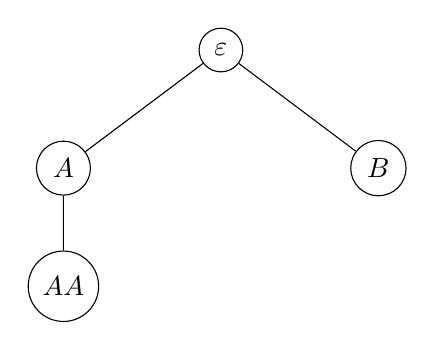
\begin{tikzpicture}[level/.style={sibling distance=40mm/#1}]
		\node [circle,draw] (epsilon){$\varepsilon$}
		child { node [circle,draw] (A) {$A$} 
			child { node[circle,draw](AA){$AA$}  }
		}
		child {node [circle,draw] (B) {$B$} }
		;
		
		\end{tikzpicture}
	\caption{Ejemplo de modelo de predicción basado en un \trie con \texttt{LZ78}.}
	\label{fig:sim}
\end{figure}



Podemos ver que a menor cantidad de símbolos en la sesión generan un árbol de menor altura y menos nodos, cada nodo como se ha señalado en el capitulo 4 representa un visita a una sección en particular de la web de \emph{MSNBC}. Cuando un \webasccesslog posee  pocas secciones o páginas visitadas, la proyección de probabilidades de los posibles símbolos en el alfabeto hace que la probabilidad del siguiente acceso sea equiprobable dentro del los símbolos de nuestro diccionario, de lo anterior convergemos en que mayor es el entrenamiento mejor será la predicción.

Dado el evento $x$  a predecir que pertenece a una secuencia discreta, la probabilidad de $P( x| AB  ) = A $, es el resultado de esta sesión de entrenamiento, pero la probabilidad $P(x | AAB) $, es desconocida.  Si extendemos los símbolos de este nodo cada nodo hijo tendría un probabilidad de $ \dfrac{1}{\Sigma} = \dfrac{1}{17} = 0.0588 $ o bien sería  $\dfrac{1}{ |\sigma| }$, siendo $|\sigma|$ el total de símbolos que se encuentran en el alfabeto. 

Para corroborar este comportamiento haremos distintos experimentos en distintos volúmenes de datos, usaremos una validación cruzada para medir el \emph{Accuracy}, la cual será nuestra métrica a utilizar.

Con esto demostraremos que secuencias con menores cantidad de símbolos generar un tipo de ruido a la métrica  que afecta en su a nuestra exactitud esperada, cuando hacemos nuevos ciclos de evaluaciones sobre el mayor orden, por otra parte veremos como con una menor cantidad de sesiones de entrenamiento podemos lograr un \emph{Accuracy} bastante optimista.



\vspace{1cm}
\begin{enumerate}
	% Idea de experimento con disminución del tamaño del alfabeto
	\item\label{exp1} \textbf{Experimento con sesiones de usuarios con datos generados de forma sintética}
	
	Creamos un set de datos en el cual pudiésemos esperar valores conocidos. Además acotamos a un diccionario de solo tres elementos, el Accurracy obtenido es:
	
	
	
	\begin{figure}[h] 
		\centering
			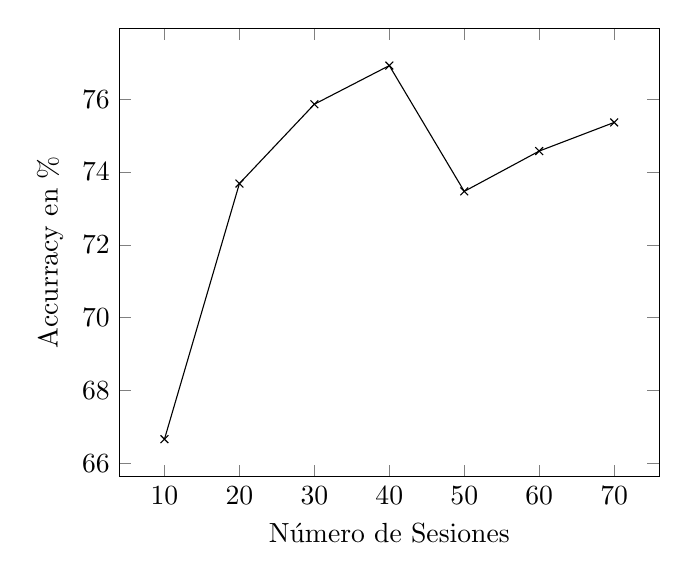
\begin{tikzpicture}
			\begin{axis}[
			xlabel= Número de Sesiones,
			ylabel=Accurracy en \% ]
			\addplot[color=black,mark=x] coordinates {
				(10, 66.6666666666666)
				(20, 73.6842105263157)
				(30, 75.8620689655172)
				(40, 76.9230769230769)
				(50, 73.469387755102)
				(60, 74.5762711864406)
				(70, 75.3623188405797)
			};
			\end{axis}
			\end{tikzpicture}	
		\caption{Experimento con set de datos sintéticos.}
		\label{fig:graph-exp1}
	\end{figure}
	

	
 
	
	En el gráfico \ref{fig:graph-exp1} usamos como mínimo 10 sesiones de las 80 de disponibles que se usaron par este experimento. Dado a que en este caso la cantidad de sesiones es bien reducida y cada símbolo posee una gran frecuencia existe mayor redundancia de datos y nuestro modelo se comporta como espera que lo haga un algoritmo de compresión de datos. Entre mayor es la cantidad de símbolos iguales
	que van entrenando al \emph{trie}, hay una aglomeración de frecuencia en ciertos nodos, pero estos son minimizados por los niveles que genera al momento de la construcción del árbol.
	
	La tasa de frecuencia de un símbolo converge a predicciones de secuencias evaluadas que caen en el nodo con mejor probabilidad dado $\epsilon$ (raíz del \emph{trie}).
	



	
   \begin{figure}[h] 
	   \centering
	   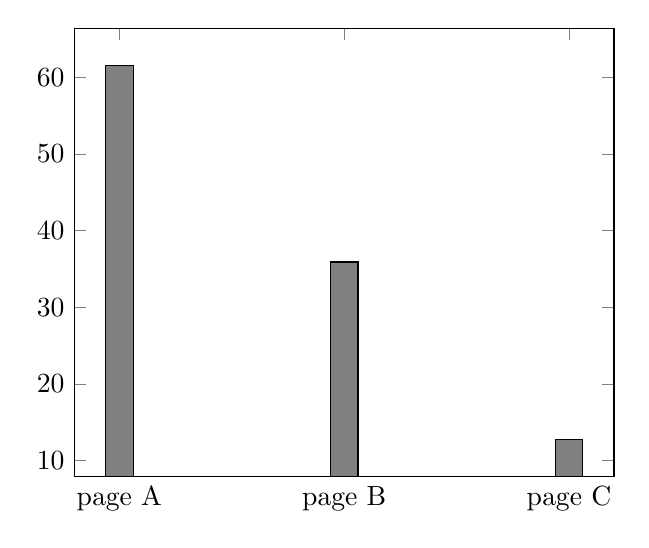
\begin{tikzpicture}
	   \begin{axis}[
	   symbolic x coords={ page A, page B, page C},
	   xtick=data
	   ]
	   \addplot[ybar,fill=gray] coordinates {
	   	(page A,   61.5)
	   	(page B,  35.9)
	   	(page C,   12.8)
	   };
	   \end{axis}
	   \end{tikzpicture}
		\caption{Distribución de símbolos para set de datos sintéticos.}
		\label{fig:bar-chart-data-sintetica}
	\end{figure}


	\begin{table}[]
		\centering
		\label{tabla-exp-1}
		\begin{tabular}{ccccc}
			\textbf{pruebas}     & \textbf{entrenamiento} & \textbf{accuracy}    & \textbf{nodos}       & \textbf{niveles}     \\
			10                   & 90                     & 0,753623188405797    & 10                   & 5                    \\
			20                   & 80                     & 0,745762711864406    & 10                   & 5                    \\
			30                   & 70                     & 0,73469387755102     & 10                   & 5                    \\
			40                   & 60                     & 0,769230769230769    & 10                   & 5                    \\
			50                   & 50                     & 0,758620689655172    & 10                   & 5                    \\
			60                   & 40                     & 0,736842105263157    & 10                   & 5                    \\
			70                   & 30                     & 0,666666666666666    & 10                   & 5                    \\
			&                        &                      &                      &                      \\
			\multicolumn{1}{l}{} & \multicolumn{1}{l}{}   & \multicolumn{1}{l}{} & \multicolumn{1}{l}{} & \multicolumn{1}{l}{}
		\end{tabular}
		\caption{ Resumen de datos experimento 1}
	\end{table}






	\begin{table}[] 	\label{tabl-exp-1-frec}
		\centering
		\resizebox{0.9\textwidth}{!}{% <------ Don't forget this %
	
		\begin{tabular}{lccccccccccccccccc}
			\textbf{símbolo}    & A  & B  & C  & D  & E & F  & G  & H  & I  & J  & K & L  & M  & N  & O & P & Q \\
			\textbf{frecuencia} & 400 & 280 & 100 & 0 & 0 & 0 & 0 & 0 & 0 & 0 & 0 & 0 & 0 & 0 & 0 & 0 & 0
		\end{tabular}
		
	}
		\caption{Tabla de frecuencia experimento 1}
	\end{table}



	Tal como se puede ver en el gráfico \ref{fig:bar-chart-data-sintetica} existe un gran probabilidad de que dado una secuencia de accesos después de $\epsilon$ la próxima sección a acceder sea la página A.
	Esto es adicionalmente es consistente a el tipo de set de datos que hemos ocupado ya que con esto podemos delimitar a que nuestro modelo al tener símbolos bastante frecuente no crea un trie desbalanceado, para este caso solo acota constantemente a un altura de 5 niveles y una variación mínima entre la exactitud, que posee el entrenamiento versus set de evaluaciones, incluso podemos solo podemos usar un entrenamiento de por lo menos 30 sesiones para predecir 50 sesiones con un Accurracy con un margen de error máximo de $10\%$ en el peor de los casos. 
	Lo anterior si lo comparamos con un evento aleatorio como resultado nos daría que nuestro modelo es bastante mejor que una predicción aleatoria, es decir $ 66.7\%  \geq 33\%$, siendo esta una comparativa optimista de que al menos nuestro modelo dado un set de datos artificial.
	



	
	
	
	\newpage
	\item \label{exp2} \textbf{Sesiones con menor redundancia y  largo variable }
		
	Validaremos ahora el comportamiento de nuestro modelo con datos reales con secuencias discretas distribuidas no uniformemente.
	
	
	
	\begin{figure}[h] 
		\centering
				\resizebox{0.6\textwidth}{!}{% <------ Don't forget this %
			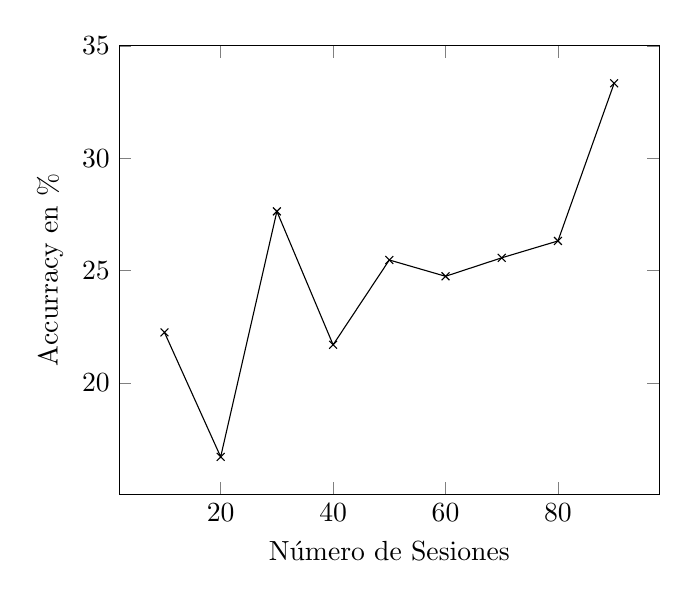
\begin{tikzpicture}
			\begin{axis}[
			xlabel= Número de Sesiones,
			ylabel=Accurracy en \% ]
			\addplot[color=black,mark=x] coordinates {
				(10, 22.2471910112359)
				(20, 16.7088607594936)
				(30, 27.6328502415459)
				(40, 21.6949152542372)
				(50, 25.469387755102)
				(60, 24.7435897435897)
				(70, 25.5665024630541)
				(80, 26.3157894736842)
				(90, 33.3333333333333)
			};
			\end{axis}
			\end{tikzpicture}
		}
		\caption{Experimento con secuencias de largo variable}
		\label{fig:experimento2}
	\end{figure}
	

	\begin{table}[h]
		\centering
		\label{tabla-exp-1}
		\begin{tabular}{ccccc}
			\textbf{pruebas}     & \textbf{entrenamiento} & \textbf{accuracy}    & \textbf{nodos}       & \textbf{niveles}     \\
			10                   & 90                     & 0,222471910112359    & 10                   & 5                    \\
			20                   & 80                     & 0,167088607594936    & 10                   & 5                    \\
			30                   & 70                     & 0,27632850241546     & 10                   & 5                    \\
			40                   & 60                     & 0,21694915254237     & 10                   & 5                    \\
			50                   & 50                     & 0,25469387755102     & 10                   & 5                    \\
			60                   & 40                     & 0,24743589743590   	 & 10                   & 5                    \\
			70                   & 30                     & 0,255665024630541    & 10                   & 5                    \\
			80                   & 20                     & 0,263157894736842    & 10                   & 5                    \\
			90                   & 10                     & 0,333333333333333    & 10                   & 5                    \\
			&                        &                      &                      &                      \\
			\multicolumn{1}{l}{} & \multicolumn{1}{l}{}   & \multicolumn{1}{l}{} & \multicolumn{1}{l}{} & \multicolumn{1}{l}{}
		\end{tabular}
		\caption{ Resumen de datos experimento 1}
	\end{table}



	\begin{table}[h] 	\label{tabl-exp-1-frec}
		\centering
		\resizebox{0.9\textwidth}{!}{% <------ Don't forget this %
	
		\begin{tabular}{lccccccccccccccccc}
			\textbf{símbolo}    & A  & B  & C  & D  & E & F  & G  & H  & I  & J  & K & L  & M  & N  & O & P & Q \\
			\textbf{frecuencia} & 64 & 19 & 18 & 29 & 4 & 36 & 20 & 65 & 20 & 11 & 4 & 15 & 42 & 31 & 2 & 0 & 0
		\end{tabular}
		
	}
		\caption{Tabla de frecuencia experimento 1}
	\end{table}


			
	En este caso si existe una menor redundancia a diferencia del experimento \ref{exp1} lo que produce que el modelo $M$ tenga un bajo rendimiento, aún así dada sigue siendo en el mejor de los casos seis veces mejor que la probabilidad aleatoria de predecir. En este experimento usamos un $|\sigma| =15$, por ende tenemos que dado nuestro modelo,
	\begin{equation}\label{expResult2}
		M( x | \mbox{90\% train}  ) = 33 \% \geq M( x | \mbox{random}  ) = 6.66 ,\% 
	\end{equation} como hemos visto en el experimento \ref{exp1} nuestro modelo sigue siendo válido en un escenario en que los datos se dispersan considerablemente. 
	Adicionalmente en este tipo de caso existe un comportamiento de nuestro modelo en el cual hace el mejor esfuerzo por mantener la \emph{compresibilidad} de los datos mayor o igual a la \emph{predictibilidad} del mismo, peor al tener mayor dispersión la altura para una cantidad similar de sesiones en \ref{exp1} sigue siendo $5$. Pero la cantidad de nodos sufre un gran incremento, podemos verlo en \ref{fig:exp-largo-variable-inf}
	
	
	
	\begin{figure}[h] 
		\centering
		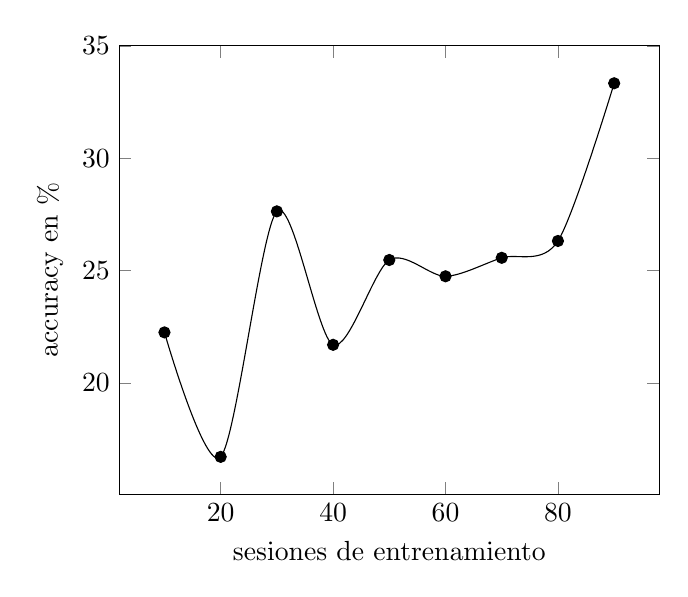
\begin{tikzpicture}
		\begin{axis}[
		xlabel=$\mbox{sesiones de entrenamiento}$,
		ylabel=$\mbox{accuracy en \%}$]
		\addplot[smooth,mark=*,black] plot coordinates {
			(10, 22.2471910112359)
			(20, 16.7088607594936)
			(30, 27.6328502415459)
			(40, 21.6949152542372)
			(50, 25.469387755102)
			(60, 24.7435897435897)
			(70, 25.5665024630541)
			(80, 26.3157894736842)
			(90, 33.3333333333333)
		};
		\end{axis}
		\end{tikzpicture}	
		
		\caption{Experimento con secuencias de largo variable inferiores y 100 sesiones}
		\label{fig:exp-largo-variable-inf}
	\end{figure}
	
	
	



	Acorde al gráfico \ref{fig:exp-largo-variable-inf} podemos señalar que al haber un incremento en la dispersión de datos y menor redundancia, el crecimiento de nuestro árbol será horizontal, ya que para tanto como hemos en este experimento y en (\label{expResult2}), la altura del nodo no tiene una relación directa a la redundancia ó dispersión, pero si a la cantidad de sesiones evaluadas. 
	
	Además, al mayor esfuerzo que hace el predictor por lograr mejores resultados se construyen mas nodos, por lo que el modelo LDC, deja de comprimir por satisfacer las condiciones de predictibilidad necesarias para seguir siendo válido.

	
	Iteramos una nueva evaluación con las mismas condiciones pero subiendo el volumen de datos de 100 a 1000. Con este buscaremos ver encontrar el mismo comportamiento a un mayor nivel de datos.
	


	
	
	\begin{figure}[t] 
		\centering
		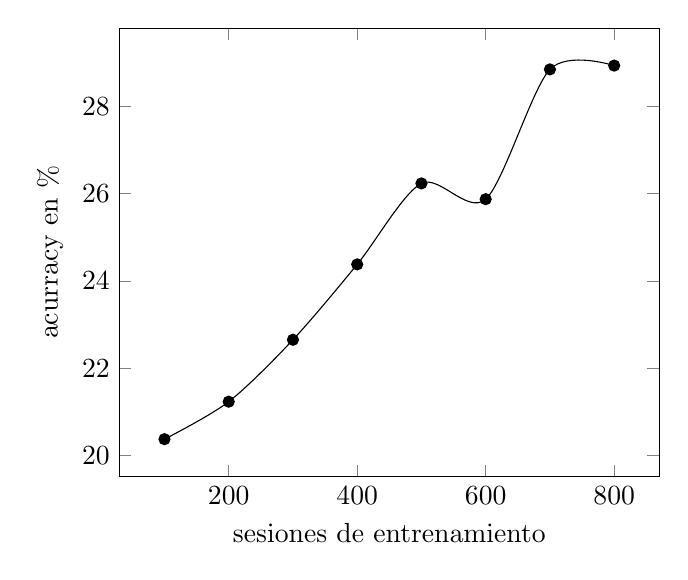
\begin{tikzpicture}
		\begin{axis}[
		xlabel=$\mbox{sesiones de entrenamiento}$,
		ylabel=$\mbox{acurracy en \%}$]
		\addplot[smooth,mark=*,black] plot coordinates {
			(100,  20.3715239154616)
			(200,  21.2302878598247)
			(300,  22.6490224129709)
			(400,  24.3752086811352)
			(500,  26.2308617234469)
			(600,  25.8692564745196)
			(700,  28.8423315814619)
			(800,  28.929431438127)
		};
		\end{axis}
		\end{tikzpicture}
		\caption{Experimento con secuencias de largo variable inferiore y 1000 sesiones}
		\label{fig:sim}
	\end{figure}
	
	El modelo sigue siendo válido al ir aumentando el volumen de datos bajo las mismas circunstancias. Incluso para ambos experimentos anteriores podemos sacar la relación que nuestro modelo posee una tasa de error de $\pm4\%$ al aumentar $100$ veces con respecto a la primera iteración de este escenario cuando se usa la  mayor cantidad de sesiones de entrenamiento posible.


	Otra particularidad que ha demostrado el modelo gracias a las propiedades de compresibilidad expuestas por  \emph{Lempel} \& \emph{Ziv}\cite{ZivLempel1977} es la minimización de niveles requeridos aún cuando la cantidad de nodos va creciendo.
	
	
	
	
	\begin{figure}[h] 
		\centering
			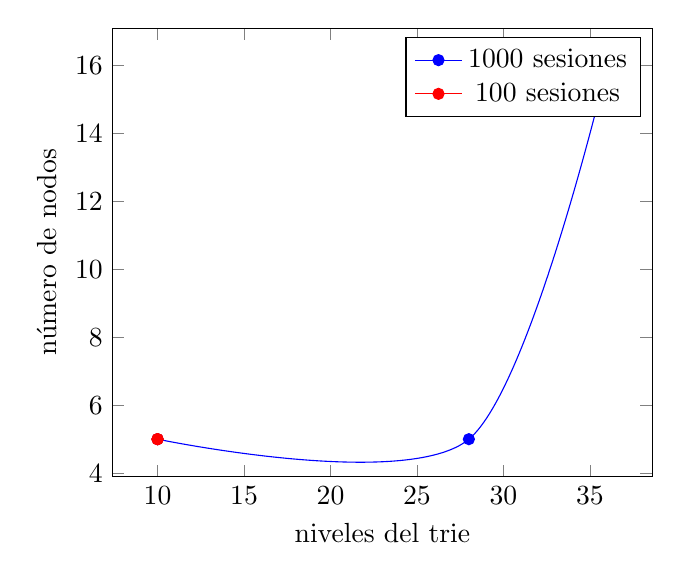
\begin{tikzpicture}
			\begin{axis}[
			xlabel=$\mbox{niveles del trie}$,
			ylabel=$\mbox{número de nodos}$]
			\addplot[smooth,mark=*,blue] plot coordinates {
				( 10 , 5 )
				( 28 , 5)
				( 36 , 16)
			};
			\addlegendentry{ 1000 sesiones }
			\addplot[smooth,mark=*,red] plot coordinates {
				( 10,5 )
				( 10,5 )
				( 10,5 )
			};
			\addlegendentry{ 100 sesiones }
			\end{axis}
			\end{tikzpicture}
		\caption{Gráfico comparativo para mismos niveles distinta cantidad de nodos.}
		\label{fig:sim}
	\end{figure}
	
	


	Como podemos ver en el comportamiento de inicio del modelo el criterio de partida en el escenario descrito es compartido por ambos experimentos.

	También dado a que no es uno de los escenarios más favorables para nuestro modelo predictivo, podríamos tener un diferencial en los tiempos de construcción del \emph{trie} respecto a la cantidad de nodos necesarios para el entrenamiento, 

	\begin{figure}[h] 
	\centering
	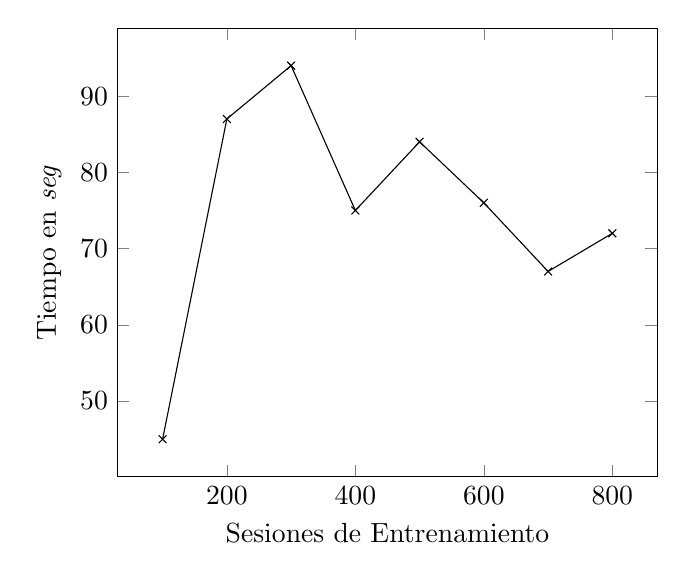
\begin{tikzpicture}
	\begin{axis}[
		xlabel= Sesiones de Entrenamiento ,
		ylabel= Tiempo en \emph{seg} ]
	\addplot[color=black,mark=x] coordinates {
			(100, 45 )
			(200, 87 )
			(300, 94 )
			(400, 75 )
			(500, 84 )
			(600, 76 )
			(700, 67)
			(800, 72 )
	};
	\end{axis}
	\end{tikzpicture}
		\caption{Gráfico de tiempo de construcción vs sesiones de entrenamiento}
	  \label{fig:sim}
	 \end{figure}	
	
	Como podemos ver en el gráfico anterior podemos buscar un dataset óptimo el cual puede encontrarse dentro del intervalo $ [ 300,400 ]$ sesiones de usuario, equivalente a la mejores resultados de \emph{Accurracy} y menor cantidad de secuencias de entrenamiento.


	\item \label{exp3}	
	\textbf{Sesiones con tamaño de secuencia constante}
	En este experimentos queremos lograr el mismo comportamiento que tuvimos en el experimento [\ref{exp1}]. Haciendo un filtrado simple de los \emph{webaccess log } que hemos estado analizando podemos llegar a mejores valores que las predicciones de resultado aleatorio.





	\begin{figure}[t] 
		\centering
			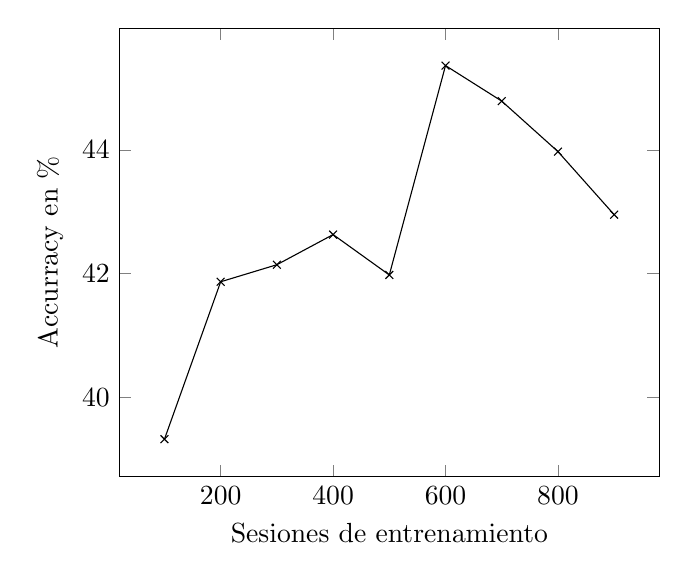
\begin{tikzpicture}
			\begin{axis}[
			xlabel=Sesiones de entrenamiento,
			ylabel=Accurracy en \% ]
			\addplot[color=black,mark=x] coordinates {
				(100, 39.3259176863181 )
				(200, 41.8698372966207 )
				(300, 42.1454458750596 )
				(400, 42.6323038397328 )
				(500, 41.9799599198396 )
				(600, 45.3634085213033 )
				(700, 44.7892976588628)
				(800, 43.9736180904522 )
				(900, 42.9539842873176 )
			};
			\end{axis}
			\end{tikzpicture}
		\caption{Gráfico de Accuracy vs sesiones de largo constante}
		\label{fig:sim}
	\end{figure}


\begin{table}[h] \label{my-label}
	\centering
	\resizebox{1\textwidth}{!}{
	\begin{tabular}{ccccc}
		\textbf{pruebas}     & \textbf{entrenamiento} & \textbf{accuracy}    & \textbf{nodos}       & \textbf{niveles}     \\
		800                  & 100                    & 0,203715239154616    & 150                  & 5                    \\
		700                  & 200                    & 0,212302878598247    & 150                  & 5                    \\
		600                  & 300                    & 0,226490224129709    & 300                  & 16                   \\
		500                  & 400                    & 0,243752086811352    & 1005                 & 48                   \\
		400                  & 500                    & 0,262308617234469    & 1005                 & 48                   \\
		300                  & 600                    & 0,258692564745196    & 1015                 & 48                   \\
		200                  & 700                    & 0,288423315814619    & 1023                 & 48                   \\
		100                  & 800                    & 0,28829431438127     & 1023                 & 48                   \\
		\multicolumn{1}{l}{} & \multicolumn{1}{l}{}   & \multicolumn{1}{l}{} & \multicolumn{1}{l}{} & \multicolumn{1}{l}{}
	\end{tabular}
	}
		\caption{Tabla resumen de experimento 3}
\end{table}

	
\begin{table}[]
	\centering \label{freq:exp3}
	\resizebox{1\textwidth}{!}{
	\begin{tabular}{lccccccccccccccccc}
		\textbf{símbolo}    & A   & B    & C   & D   & E   & F    & G   & H   & I   & J    & K   & L   & M   & N    & O  & P  & Q  \\
		\textbf{frecuencia} & 861 & 1502 & 509 & 412 & 557 & 1163 & 557 & 626 & 272 & 2252 & 399 & 703 & 301 & 1889 & 67 & 57 & 98
	\end{tabular}
	}
		\caption{Frecuencia de símbolos para experimentos con sesiones de largo constante.}	
	
\end{table}	
	
	
	La cantidad total de sesiones usadas fueron $1.000$ y las cuales como en el gráfico anterior se señala a mayor cantidad entrenamiento existe al menos un punto de la curva que se vuelve un máximo.


	Seguido a esto podemos ver el tiempo de construcción del \emph{trie} que nuestro modelo demora en generar:
	
	
	
	\begin{figure}[h] 
		\centering
		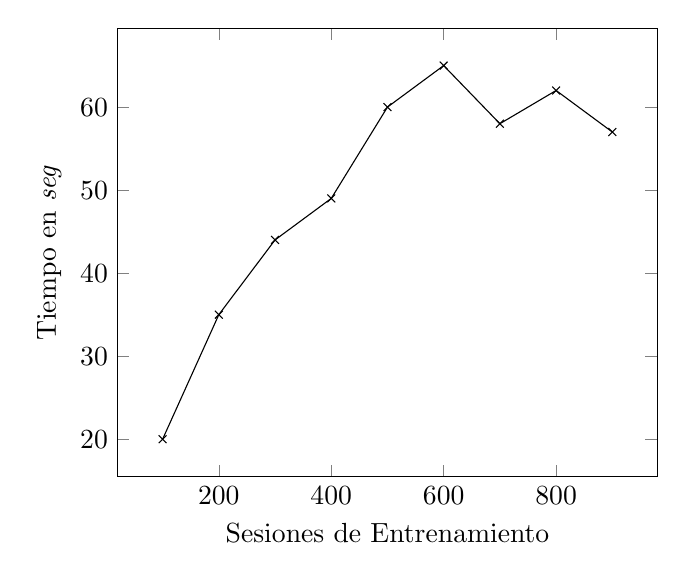
\begin{tikzpicture}
		\begin{axis}[
		xlabel= Sesiones de Entrenamiento ,
		ylabel=Tiempo en \emph{seg} ]
		\addplot[color=black,mark=x] coordinates {
			(100, 20)
			(200, 35)
			(300, 44)
			(400, 49)
			(500, 60)
			(600, 65)
			(700, 58)
			(800, 62)
			(900, 57 )
		};
		\end{axis}
		\end{tikzpicture}
		\caption{Gráfico de Tiempo vs sesiones de largo constante}
		\label{fig:sim}
	\end{figure}
	
	

	Al igual que en el gráfico anterior podemos ver que existe al menos una mínima cantidad sesiones las cuales generar un rendimiento sobre las evaluaciones a realizar. 
	

	\item \label{exp4} \textbf{Secuencias de accesos con limite inferior 100 símbolos }
	Este experimento busca validar las condiciones necesarias que debe tener una secuencia de entrada para que el algoritmo \texttt{LDC} pueda optimizar al momento de ser construido para una predicción \emph{online}, dado esto utilizaremos sesiones largas que entreguen redundancia en los accesos que permita al modelo de navegación ser más comprimido sin perder una métrica considerable para funcionar, según lo anterior realizamos las siguientes particiones de data que cumplen en el siguiente ciclo. 
	
	\begin{figure}[h] 
		\centering
		\resizebox{.7\textwidth}{!}{
		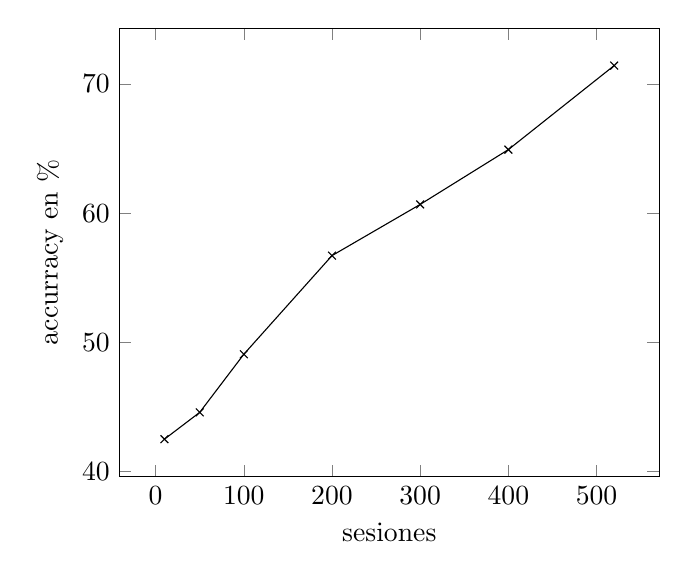
\begin{tikzpicture}
		\begin{axis}[
			xlabel= sesiones,
			ylabel=accurracy en \% ]
		\addplot[color=black,mark=x] coordinates {
			(10 ,  42.5190839694656 )
			(50 ,  44.595041322314 )
	 		(100 , 49.089861751152 )
	 		(200 , 56.7230538922155 )
	 		(300 , 60.6837606837608 )
	 		(400 , 64.9253731343282 )
	 		(520 , 71.4285714285715 )			
		};
		\end{axis}
		\end{tikzpicture}
		}
		\caption{Gráfico de Accuracy para sesiones mayores de 100 símbolos}
		\label{fig:sim}
	\end{figure}
	
	
	Sean la sesiones de entrenamiento de tamaño $T$, con un valor  $T(100) = 49 \% $ sobre un set de evaluación $E(100) = 900 \mbox{ sesiones}$ , nuestro modelo propuesto al igual que en el experimento \ref{exp1}, entrega un punto mínimo el cual al menos da un $50\%$ de acierto sobre el total de $535$ sesiones de usuarios, con una secuencia mínima de $100$ símbolos. Planteado de otra forma, sólo con el $20\%$ del total de datos de entrenamiento nuestro motor de predicción ya alcanza un \emph{Accurracy} que es mucho mejor que un predictor aleatorio sobre el alfabeto del experimento. Siendo este valor bastante optimista acorde a los puntos óptimos del predictor que use la menor cantidad de recursos.
	
	
	\begin{figure}[h] \label{fig:sim}
	\centering
		\resizebox{.7\textwidth}{!}{
		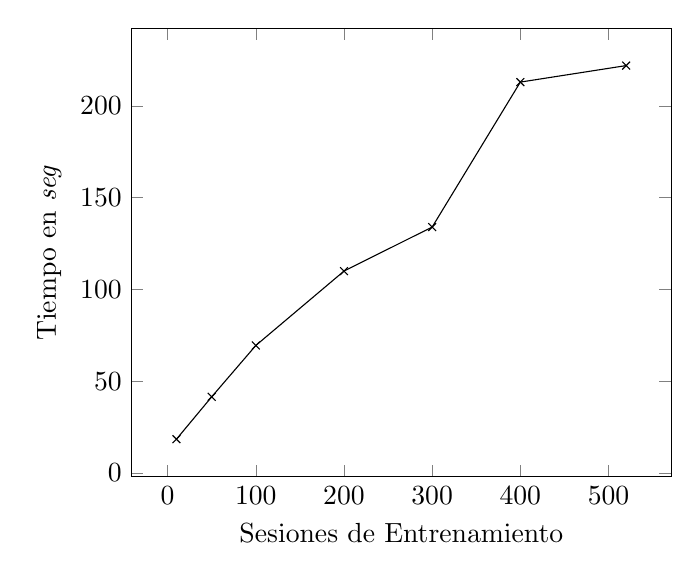
\begin{tikzpicture}
		\begin{axis}[
		xlabel= Sesiones de Entrenamiento ,
		ylabel=Tiempo en \emph{seg} ]
		\addplot[color=black,mark=x] coordinates {
			(10 ,  18.4)
			(50 ,  41.5)
			(100 , 69.46)
			(200 , 110)
			(300 , 134)
			(400 , 213)
			(520 , 222)	
		};
		\end{axis}
		\end{tikzpicture}
		}
		\caption{Gráfico de tiempo vs sesiones de entrenamiento\\ para sesiones mayores de 100 símbolos}
		
	\end{figure}


\begin{table}[h]
	\centering
	\caption{Tabla resumen experimento 4}
	\label{my-label}
	\begin{tabular}{ccccc}
		\textbf{pruebas} & \textbf{entrenamiento} & \textbf{accuracy} & \textbf{nodos} & \textbf{niveles} \\
		990              & 10                     & 0,21422649140546  & 38             & 5                \\
		950              & 50                     & 0,3104531085353   & 95             & 5                \\
		900              & 100                    & 0,393259176863181 & 132            & 5                \\
		800              & 200                    & 0,418698372966207 & 181            & 5                \\
		700              & 300                    & 0,421454458750596 & 208            & 5                \\
		600              & 400                    & 0,426323038397328 & 241            & 5                \\
		500              & 500                    & 0,419799599198396 & 264            & 5                \\
		400              & 600                    & 0,453634085213033 & 288            & 5                \\
		300              & 700                    & 0,407892976588628 & 308            & 5                \\
		200              & 800                    & 0,439736180904522 & 326            & 5                \\
		100              & 900                    & 0,429539842873176 & 349            & 5               
	\end{tabular}
\end{table}

\begin{table}[]
	\centering

	\label{my-label}
	\resizebox{0.9\textwidth}{!}{
	\begin{tabular}{lccccccccccccccccc}
		\textbf{símbolo}    & A    & B    & C   & D   & E   & F   & G   & H    & I   & J   & K   & L   & M   & N   & O   & P  & Q  \\
		\textbf{frecuencia} & 2162 & 1044 & 269 & 757 & 225 & 815 & 681 & 1207 & 370 & 278 & 233 & 453 & 502 & 860 & 102 & 10 & 32
	\end{tabular}
	}
	\caption{Tabla resumen de simbolos y frecuencia para experimento 4}
\end{table}

	Congruente con lo anterior podemos ver que sin tener un margen de error superior a la porción de datos seleccionado logramos un latencia de consulta predictiva en línea de alrededor de 70 \emph{seg}, el cual para ser implementado y consumido como ya se había mencionado antes como un algoritmo predictivo como servicio \texttt{REST}, esta dentro del promedio aceptable.

	\begin{figure}[h] 
		\centering
		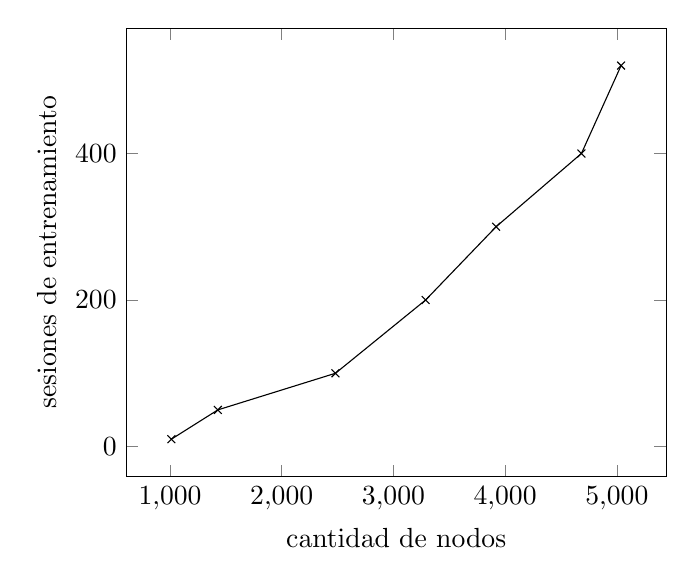
\begin{tikzpicture}
		\begin{axis}[
			xlabel= cantidad de nodos,
			ylabel= sesiones de entrenamiento  ]
		\addplot[color=black,mark=x] coordinates {
			(1012,10 )
			(1428,50 )
			(2481,100 )
			(3288,200 )
			(3919,300 )
			(4683,400 )
			(5038,520 )	
		};
		\end{axis}
		\end{tikzpicture}	
		\caption{Gráfico de cantidad de nodos vs sesiones de entrenamiento para sesiones mayores de 100 símbolos}
	  \label{fig:sim}
	\end{figure}


	Otro de los puntos  considerado aceptable, es que dado un set de entrenamiento $T(100)$, solo necesitaremos menos de la mitad de nodos que se requieren para llegar a un valor de predicción bueno, a diferencia de una partición de entrenamiento que requiere más del $90\%$ de nodos del total del set de datos.\\
	

	
	\begin{figure}[h] 
		\centering
			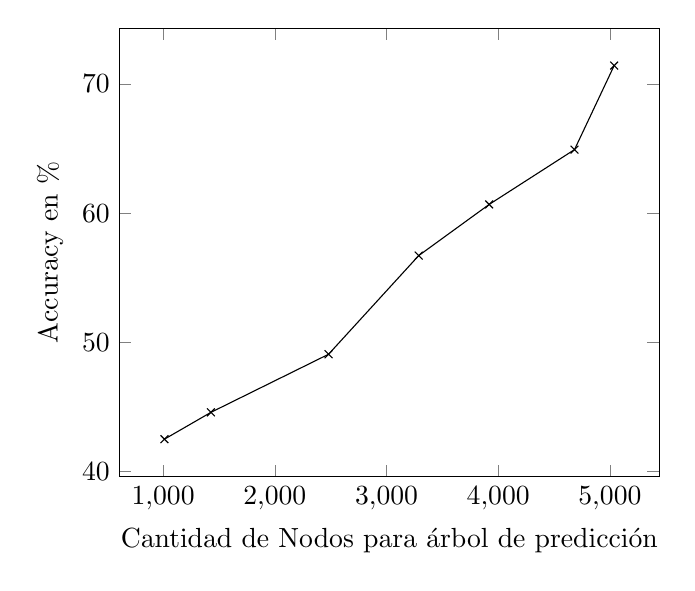
\begin{tikzpicture}
			\begin{axis}[
			xlabel=Cantidad de Nodos para árbol de predicción,
			ylabel=Accuracy en \%  ]
			\addplot[color=black,mark=x] coordinates {
				(1012,42.5190839694656 )
				(1428,44.595041322314 )
				(2481,49.089861751152 )
				(3288,56.7230538922155 )
				(3919,60.6837606837608 )
				(4683,64.9253731343282 )
				(5038,71.4285714285715 )	
			};	
			\end{axis}
			\end{tikzpicture}	
			\caption{Gráfico de cantidad de nodos vs Accuracy para sesiones mayor de 100 símbolos}
		\label{fig:sim}
	\end{figure}



	Finalmente podemos señalar que la tasa de \emph{Accuracy}, aún  subiendo al doble la cantidad de nodos para construir un \emph{trie} de \texttt{LZ78}, con mayor información  para predecir alcanza un rendimiento aceptable respecto de la compresión realizada. De todas maneras también se cumple que la cantidad de nodos del entrenamiento es directamente proporcional a la métrica seleccionada.


	\item \label{exp5}	
	\textbf{Sesiones con menos de 5 \emph{webaccess} para generar el \emph{trie}}
		Hacemos una validación cruzada para una muestra de data de 906130 sesiones de usuarios para probar como se comporta con {cross validation}.
	
	
	\begin{table}[tb]
		\centering
		\label{my-label}
				\resizebox{0.9\textwidth}{!}{
		\begin{tabular}{ccccc}
			\textbf{pruebas} & \textbf{entrenamiento} & \textbf{accuracy} & \textbf{nodos} & \textbf{niveles} \\
			990              & 10                     & 0,425190839694656 & 38             & 5                \\
			950              & 50                     & 0,44595041322314  & 95             & 5                \\
			900              & 100                    & 0,49089861751152  & 132            & 5                \\
			800              & 200                    & 0,567230538922155 & 181            & 5                \\
			700              & 300                    & 0,606837606837608 & 208            & 5                \\
			600              & 400                    & 0,649253731343282 & 241            & 5                \\
			500              & 520                    & 0,714285714285715 & 264            & 5               
		\end{tabular}
	}
			\caption{Tabla resumen experimento 6}
	\end{table}
	
	
	
	
	\begin{table}[tb]
		\centering
		\caption{Tabla resumen para sesiones mayores de 100000 sesiones}
		\label{my-label}
		\resizebox{.8\textwidth}{!}{
		\begin{tabular}{ccccc}
			\textbf{pruebas} & \textbf{entrenamiento}  & \textbf{accuracy} & \textbf{nodos} & \textbf{niveles} \\
			990              & 100                     & 0,299674371114825  & 61            & 4               \\
			950              & 200                     & 0,449237667712101  & 108           & 5               \\
			900              & 1000                    & 0,56519572924979   & 242           & 5               \\
			800              & 2500                    & 0,689237667712101  & 336           & 5               

		\end{tabular}
		}
	\end{table}
	
	
	
	\begin{figure}[h] 
		\centering
			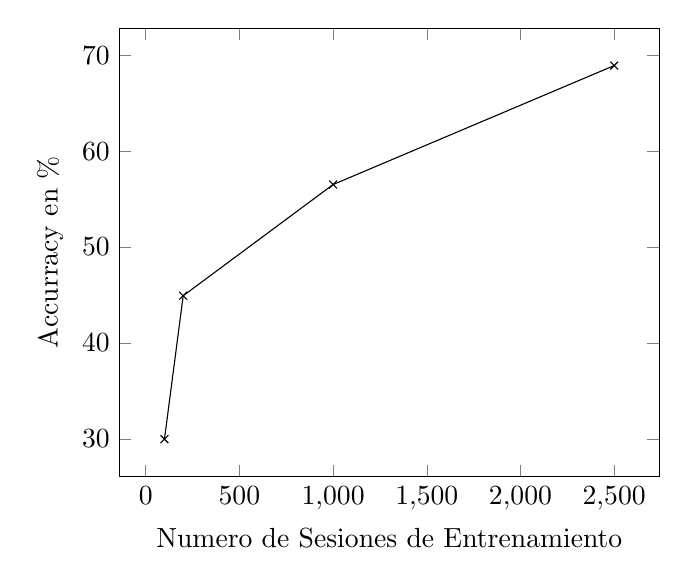
\begin{tikzpicture}
			\begin{axis}[
			xlabel= Numero de Sesiones de Entrenamiento,
			ylabel=Accurracy en \% ]
			\addplot[color=black,mark=x] coordinates {
				(100, 29.9674371114825)
				(200, 44.9237667712101)
				(1000, 56.519572924979)
				(2500, 68.9237667712101)	
			};
			\end{axis}
			\end{tikzpicture}
		\caption{Gráfico de Accuracy vs sesiones de entrenamiento para una cota superior de 5 símbolos}
		\label{fig:sim}
	\end{figure}
	
	\begin{table}[]
		\centering

		\label{my-label}
		\resizebox{1\textwidth}{!}{
		\begin{tabular}{lccccccccccccccccc}
			\textbf{símbolo}                                                                  & A                         & B                         & C                         & D                         & E                        & F                         & G                        & H                         & I                         & J                        & K                        & L                         & M                         & N                         & O                        & P                       & Q                       \\
			\textbf{\begin{tabular}[c]{@{}l@{}}frecuencia \\ 1000 sesiones\end{tabular}}      & 31086                     & 14262                     & 5483                      & 15458                     & 12713                    & 7717                      & 8255                     & 4155                      & 2381                      & 9697                     & 1974                     & 9584                      & 1871                      & 12795                     & 3935                     & 11735                   & 506                     \\
			\textbf{\begin{tabular}[c]{@{}l@{}}frecuencia \\ 100.000\\ sesiones\end{tabular}} & \multicolumn{1}{l}{43173} & \multicolumn{1}{l}{20251} & \multicolumn{1}{l}{15093} & \multicolumn{1}{l}{12790} & \multicolumn{1}{l}{1458} & \multicolumn{1}{l}{26517} & \multicolumn{1}{l}{4154} & \multicolumn{1}{l}{14517} & \multicolumn{1}{l}{12262} & \multicolumn{1}{l}{4163} & \multicolumn{1}{l}{4658} & \multicolumn{1}{l}{13180} & \multicolumn{1}{l}{14021} & \multicolumn{1}{l}{15779} & \multicolumn{1}{l}{2498} & \multicolumn{1}{l}{125} & \multicolumn{1}{l}{559}
		\end{tabular}
		}
		\caption{Tabla de frecuencia de símbolos para $1.000$ sesiones y $100.000$ }
	\end{table}
	
		
	
	
	\item \label{exp6} 
	\textbf{Detección de Ruido en secuencias de acceso}
	
	Al modelar una navegación de usuario mediante un \emph{trie} basado en un algoritmo como \texttt{LZ78}, adoptamos un enfoque basado en la frecuencia por lo cual si realizamos experimentos para poder encontrar ruido veremos que que son secuencias de acceso comunes y estas no dan relevancia o aportan a la exactitud ó precisión del algoritmo.
	
	Sea la secuencia $\{A,A,A,A,A,A,A,A,A,A,A,A \}$ a la cual llamaremos secuencia $R$, si $A$ es representado por el \emph{home} ó página de inicio, esto da a interpretación que existe un usuario en su sesión $R$ que se encuentra accediendo constantemente a esta sección. Podemos señalar que esta es una sesión ruidosa si:
	
	\begin{equation}
		P( x | AAAAAAA)= A ,	
	\end{equation} pero siendo la sesión $R$ de tamaño = $12$, en el siguiente acceso tendremos una probabilidad equiprobable dentro de las secciones en nuestro alfabeto, la cual generará un probabilidad de éxito ''falso positivo''.
	
	En el siguiente experimento veremos como se comporta nuestro modelo dado entradas \emph{Ruidosas}. Además se mostrará como el árbol suele perder su balance a medida que va creciendo los niveles de altura. 
	
	
	
	Por otro lado teniendo la noción de como es el funcionamiento de un servidor \texttt{IIS}, y al ser una página con un gran número de visitas, podemos señalar que los datos proporcionados no son totalmente representativos de usuarios reales, ya que la web al bien indexada en los buscadores existen un cantidad indeterminada de \emph{Crawlers} ó \emph{Bots} que están constantemente generando accesos tanto para almacenar en caché páginas o generando accesos automatizados a ciertos secciones sin ser datos representativo. Dejamos como discusión que algoritmo se podría implementar para detección de estos patrones por las ramas que hemos generado para la detección de \emph{bots} o \emph{robots}.
	
	
	
	
	 
	
	%	\item  Dataset uniformes de largo acotado inferiormente y volumenes de alto tamaño.
\end{enumerate}








 



	% \begin{forest} 
	% 	[VP
	% 	[DP]
	% 	[V’
	% 	[V]
	% 	[DP]
	% 	]
	% 	]
	% \end{forest}



	% \begin{tikzpicture}[level/.style={sibling distance=60mm/#1}]
	% \node [circle,draw] (z){$n$}
	% child {node [circle,draw] (a) {$\frac{n}{2}$}
	% 	child {node [circle,draw] (b) {$\frac{n}{2^2}$}
	% 		child {node {$\vdots$}
	% 			child {node [circle,draw] (d) {$\frac{n}{2^k}$}}
	% 			child {node [circle,draw] (e) {$\frac{n}{2^k}$}}
	% 		} 
	% 		child {node {$\vdots$}}
	% 	}
	% 	child {node [circle,draw] (g) {$\frac{n}{2^2}$}
	% 		child {node {$\vdots$}}
	% 		child {node {$\vdots$}}
	% 	}
	% }
	% child {node [circle,draw] (j) {$\frac{n}{2}$}
	% 	child {node [circle,draw] (k) {$\frac{n}{2^2}$}
	% 		child {node {$\vdots$}}
	% 		child {node {$\vdots$}}
	% 	}
	% 	child {node [circle,draw] (l) {$\frac{n}{2^2}$}
	% 		child {node {$\vdots$}}
	% 		child {node (c){$\vdots$}
	% 			child {node [circle,draw] (o) {$\frac{n}{2^k}$}}
	% 			child {node [circle,draw] (p) {$\frac{n}{2^k}$}
	% 				child [grow=right] {node (q) {$=$} edge from parent[draw=none]
	% 					child [grow=right] {node (q) {$O_{k = \lg n}(n)$} edge from parent[draw=none]
	% 						child [grow=up] {node (r) {$\vdots$} edge from parent[draw=none]
	% 							child [grow=up] {node (s) {$O_2(n)$} edge from parent[draw=none]
	% 								child [grow=up] {node (t) {$O_1(n)$} edge from parent[draw=none]
	% 									child [grow=up] {node (u) {$O_0(n)$} edge from parent[draw=none]}
	% 								}
	% 							}
	% 						}
	% 						child [grow=down] {node (v) {$O(n \cdot \lg n)$}edge from parent[draw=none]}
	% 					}
	% 				}
	% 			}
	% 		}
	% 	}
	% };
	% \path (a) -- (j) node [midway] {+};
	% \path (b) -- (g) node [midway] {+};
	% \path (k) -- (l) node [midway] {+};
	% \path (k) -- (g) node [midway] {+};
	% \path (d) -- (e) node [midway] {+};
	% \path (o) -- (p) node [midway] {+};
	% \path (o) -- (e) node (x) [midway] {$\cdots$}
	% child [grow=down] {
	% 	node (y) {$O\left(\displaystyle\sum_{i = 0}^k 2^i \cdot \frac{n}{2^i}\right)$}
	% 	edge from parent[draw=none]
	% };
	% \path (q) -- (r) node [midway] {+};
	% \path (s) -- (r) node [midway] {+};
	% \path (s) -- (t) node [midway] {+};
	% \path (s) -- (l) node [midway] {=};
	% \path (t) -- (u) node [midway] {+};
	% \path (z) -- (u) node [midway] {=};
	% \path (j) -- (t) node [midway] {=};
	% \path (y) -- (x) node [midway] {$\Downarrow$};
	% \path (v) -- (y)
	% node (w) [midway] {$O\left(\displaystyle\sum_{i = 0}^k n\right) = O(k \cdot n)$};
	% \path (q) -- (v) node [midway] {=};
	% \path (e) -- (x) node [midway] {+};
	% \path (o) -- (x) node [midway] {+};
	% \path (y) -- (w) node [midway] {$=$};
	% \path (v) -- (w) node [midway] {$\Leftrightarrow$};
	% \path (r) -- (c) node [midway] {$\cdots$};
	% \end{tikzpicture}



%Las conclusiones son deducidas logicamen- te de los resultados obtenidos y de la interpretacionpresen- tada, ademas estan conectadas al marco teorico.
%Las conclusiones muestran el logro de los ob jetivos.
%Se presentan proyec- ciones validas y valio- sas a partir del traba- jo realizado.
%Se detallan claramen- te las limitaciones del traba jo realizado.




 


 
%%%%%%%%
%%%%%%%%


 

El orden de como se ingresan las sesiones afecta directamente proporcional a la construcción del modelo \emph{trie},  por lo cual es un factor  \emph{FIFO} al momento de crear, lo primero que lee es lo primero que entrena por lo cual se debiese tener un criterio para ordenar los \emph{webaccess} antes de poder pasarlos al entrenador, que implica antes de la construcción.

El modelo propuesto, básicamente es un compresor el cual no toma decisiones, una posible mejora sería implementar un árbol de decisiones con algún criterio para decidir que entrenar y que no, estos árboles pueden estar dentro del \emph{trie} para
poder elegir secuencias optimo acorde a los criterios históricos, así podría darse el caso de ser un compresor--predictor  \emph{mas inteligente}.










\newpage
\section{Conclusiones }\label{ch:conlusion-contrib-all}

Aún cuando se presenta varios antecedentes, podemos decir que nuestro modelo ocupa bastante menos memoria pero esto va directamente relacionado el tamaño del \emph{trie} de predicción generado.

%
Aun cuando el \emph{trie} que representa totalmente el modelo de navegación del los usuarios de un sitio web, este no puede generalizar completamente el comportamiento estocástico de los usuarios y/o agentes que acceden a los recursos de \emph{MSNBC} o un cualquier web en general.

Una de las mayores ventajas de nuestro modelo es que al estar embebido en un servidor de Machine Learning, cada nuevo evento que ingresa para la siguiente nueva ejecución esta estará mejor preparado, podríamos decir que la recolección de data de cada evento en particular nos ayudaría a que nuestro modelo en futuros trabajos vaya aprendiendo mas y más precisamente.


A medida que la altura del árbol va creciendo este genera mayor demora en cuanto a la creación del \emph{trie}.
% Pero a mayor altura hay mayor precisión.

Hemos validado que hacer un modelo de navegación de usuarios es un perfecta implementación de un predictor usando un árbol de la familia de \emph{Lempel} \& \emph{Ziv}.

A nuestro modelo le es afectado secuencias de menor tamaño, por lo cual se debe trabajar para hacer un aprendizaje de que momento omitirlo o no. Estas sesiones de bajo número de secuencias genera un bajo porcentaje de \emph{accurracy}. 


% Cual es el minimo entrenamiento para lograr a Predecir ?

Hemos presentado un modelo liviano el cual puede ser utilizado para predecir secuencias de \emph{webaccess} en demanda.






%In this paper we studied the empirical performance of a number of prominent prediction algorithms. We focused on prediction settings that are more closely related to those required

%%%%%%%%% On Prediction Using Variable Order Markov Models

%$%%%%%%%%
%%n this paper we studied the empirical performance of a number of prominent prediction algorithms. We focused on prediction settings that are more closely related to those required


%On Prediction Using Variable Order Markov Models
%by machine learning practitioners dealing with discrete sequences.
%However, somewhat surprisingly, the best predictor under the log-loss is not the best classifier. On the contrary, the consistently best protein classifier is based on the mediocre lz-ms predictor! This algo- rithm is a simple modification of the well-known Lempel-Ziv-78 (lz78) prediction algorithm, which can capture VMMs with large contexts. The surprisingly good classification accuracy achieved by this algorithm may be of independent interest to protein analysis research and clearly deserves further investigatio 
% Genero toda las referencias para demostrar el uso de la bibliografía
% No es necesario que utilice este comando en su document
%
%Conclusion of this paper Gopalratnam Cook
%a

lz modelos eficazmente procesos secuenciales, y es extremadamente útil para la predicción de los procesos donde los eventos son dependientes de la historia evento anterior. Esto es debido a la capacidad del algoritmo para construir un modelo preciso de la fuente de los eventos que se generan, una característica heredada de su información de fondo teórico y el algoritmo de compresión de texto \texttt{LZ78}.
%
La eficacia del método para el aprendizaje de una medida de tiempo también se puede atribuir a hecho de que ALZ es un fuerte predictor secuencial. Los principios teóricos de sonido en el que ALZ se fundamenta también significan que ALZ es un universal Quiniela óptima, y se puede utilizar en una variedad de escenarios de predicción.
%conclusion lcoa
%

Dado que la mayoría de los predictores funcionan de 
manera offline, uno de los aporte de tener estar estructura de algoritmos como servicios es poder tener un motor de predicción en linea.

\newpage
\section{Trabajos Futuro}

Esta memoria forma parte del plan de continuidad en el postgrado de la Escuela de Ingeniería Informática y telecomunicaciones, por lo cual se desea profundizar este trabajo en las discusiones realizadas. Los temas deseados por abarcar:

\begin{itemize}

\item Crear un estudio comparativo con Modelos de \emph{Machine Learning} como (\emph{RNN}) Redes Neuronales, Reglas de Asociación, \emph{Deep Learning} y algoritmo de tipo \emph{Frequent Pattern Growth}.

\item Técnicas para mejorar el modelo de predicción 
\item Mejorar la implementación de \texttt{LZ78}, realizado con lenguaje funcional y objetos(\emph{Scala}) y hacer una comparación de rendimientos contra implementaciones clásicas en lenguajes de más bajo nivel (\texttt{C++}).


\item Crear técnicas como la usada por \emph{Claude}~\etal~\cite{Claude2014}, para crear representaciones eficientes en función de este modelo predictivo.


\item Investigar los factores teóricos y técnicos para poder mejorar la exactitud de la predicción.

\item Ambiciosamente a realizar un estudio comparativo para encontrar puntos en común de estas áreas de la ciencia de la computación, se desea crear un nuevo algoritmo basado en la familia de \lempelziv, el cual pueda tener un complemento para la selección de sesiones antes ser ingresadas en el modelo de navegación predictivo. 


	
\end{itemize}	




%%%%%%%%%%%%%%%%%%%%%%%%%%%
% Iniciamos el resto de secciones adicionales al contenido: referencias y apendices
\backmatter
%%%%%%%%%%%%%%%%%%%%%%%%%%%
%%Se presenta una revision bibliografica acertada, actual, y exhaustiva (se consulta toda la literatura relevante).
%Presenta y redacta los objetivos, el trabajo realizado, y la validacion de manera detallada. Presenta discusiones detalladas, articuladas, claras, y un buen uso del lenguaje tecnico.
% Bibliografía - El estilo por defecto es IEEE Transactions
\bibliographystyle{ieeetr}
\bibliography{IEEEabrv,referencias}
%%%%%%%%%%%%%%%%%%%%%%%%%%%
% Simbología y glosario
% Utilice un paquete para generar símbolos y glosarios.
% Por ejemplo: nomencl (http://texdoc.net/pkg/nomencl)
% Anexos
\appendix
%%%%%%%%%%%%%%%%%%%%%%%%%%%
\chapter{Primer anexo}
\label{ch:anexo-a}


Configuraciones para hacer correr IntelliJ con Apache SPARK y Prediction.IO 0.94


\begin{lstlisting}[frame=single,basicstyle=\ttfamily\tiny,]
Main class: io.prediction.workflow.CreateWorkflow

VM options: -Dspark.master=local -Dlog4j.configuration=file:/Users/jguzman/PredictionIO/conf/log4j.properties


Program arguments: --engine-id dummy --engine-version dummy --engine-variant engine.json


io.prediction.workflow.CreateWorkflow
-Dspark.master=local -Dlog4j.configuration=file:/Users/jguzman/PredictionIO/conf/log4j.properties -Dorg.xerial.snappy.lib.name=libsnappyjava.jnilib 
--engine-id dummy --engine-version dummy --engine-variant engine.json



SPARK_HOME=/Users/jguzman/PredictionIO/vendors/spark-1.4.1/bin
PIO_FS_BASEDIR=/Users/jguzman/.pio_store
PIO_FS_ENGINESDIR=/Users/jguzman/.pio_store/engines
PIO_FS_TMPDIR=/Users/jguzman/.pio_store/tmp
PIO_STORAGE_REPOSITORIES_METADATA_NAME=pio_meta
PIO_STORAGE_REPOSITORIES_METADATA_SOURCE=ELASTICSEARCH
PIO_STORAGE_REPOSITORIES_MODELDATA_NAME=pio_model
PIO_STORAGE_REPOSITORIES_MODELDATA_SOURCE=LOCALFS
PIO_STORAGE_REPOSITORIES_APPDATA_NAME=pio_appdata
PIO_STORAGE_REPOSITORIES_APPDATA_SOURCE=ELASTICSEARCH
PIO_STORAGE_REPOSITORIES_EVENTDATA_NAME=pio_event
PIO_STORAGE_REPOSITORIES_EVENTDATA_SOURCE=HBASE
PIO_STORAGE_SOURCES_ELASTICSEARCH_TYPE=elasticsearch
PIO_STORAGE_SOURCES_ELASTICSEARCH_HOSTS=localhost
PIO_STORAGE_SOURCES_ELASTICSEARCH_PORTS=9300
PIO_STORAGE_SOURCES_LOCALFS_TYPE=localfs
PIO_STORAGE_SOURCES_LOCALFS_HOSTS=/Users/jguzman/.pio_store/models
PIO_STORAGE_SOURCES_LOCALFS_PORTS=0
PIO_STORAGE_SOURCES_HBASE_TYPE=hbase
PIO_STORAGE_SOURCES_HBASE_HOSTS=0
PIO_STORAGE_SOURCES_HBASE_PORTS=0


Main class: io.prediction.workflow.CreateServer
Program Arguments: --engineInstanceId **replace_with_the_id_from_pio_train**




Try -- for more information.
Usage: pio train [--batch <value>] [--skip-sanity-check]
                 [--stop-after-read] [--stop-after-prepare]
                 [--engine-factory <value>] [--engine-params-key <value>]
                 [--scratch-uri <value>]
                 [common options...]

Kick off a training using an engine (variant) to produce an engine instance.
This command will pass all pass-through arguments to its underlying spark-submit
command.

  --batch <value>
      Batch label of the run.
  --skip-sanity-check
      Disable all data sanity check. Useful for speeding up training in
      production.
  --stop-after-read
      Stop the training process after DataSource.read(). Useful for debugging.
  --stop-after-prepare
      Stop the training process after Preparator.prepare(). Useful for
      debugging.
  --engine-factory
      Override engine factory class.
  --engine-params-key
      Retrieve engine parameters programmatically from the engine factory class.
  --scratch-uri
      URI of the working scratch space. Specify this when you want to have all
      necessary files transferred to a remote location. You will usually want to
      specify this when you use --deploy-mode cluster.

\end{lstlisting}

\vspace{1cm}

Como hacer llamadas curl desde la consola o terminal Linux


\begin{lstlisting}

curl -H "Content-Type: application/json"  -d '{"webaccess" : "AC","num" : 10}' http://52.33.180.212:8000/queries.json



\end{lstlisting}





%\blindtext[5]


\chapter{Segundo anexo}
\label{ch:anexo-b}


%\blindtext[10]


  
%%%%%%%%%%%%%%%%%%%%%%%%%%%

\clearpage
\printglossary[type=\acronymtype]
\printglossary
\end{document}